\documentclass[a4paper,openright,11pt]{book}
\usepackage[a-1b]{pdfx}
\usepackage{lettrine,lipsum,mparhack,geometry,longtable,booktabs,caption,titlesec,graphicx}
\usepackage{microtype,mathtools,slashed,subfig,multicol}
\usepackage[version=4]{mhchem}
\usepackage{amsthm}
\usepackage{amsmath}
\usepackage[swapnames]{frontespizio}
\usepackage{tikz}
\usetikzlibrary{trees,decorations.pathmorphing,decorations.markings,shadings,patterns,quotes,angles,snakes}%snakes
\usetikzlibrary{shapes.arrows}
\usepackage[T1]{fontenc}
\usepackage[urw-garamond]{mathdesign}
\usepackage[autostyle]{csquotes}
\usepackage{dashrule}
\usepackage[backend=bibtex,bibstyle=authortitle,style=numeric-comp,sorting=none]{biblatex}
\addbibresource{bibliography.bib}

\newcommand{\ATLASLATEXPATH}{../atlaslatex/latex/}
\usepackage{\ATLASLATEXPATH atlasphysics}
\usepackage[range-phrase=-]{siunitx}
\newcommand{\gmet}{$\gamma +$\met\xspace}
\newcommand{\znng}{\mbox{$\Zboson (\rarrow \nu\nu )  + \gamma$}\xspace}
\newcommand{\zg}{\mbox{$\Zboson (\rarrow \ell\ell) + \gamma$}\xspace}
\newcommand{\wg}{\mbox{$\Wboson (\rarrow \lnu) + \gamma$}\xspace}
\newcommand{\gj}{\mbox{$\gamma + \text{jets}$}\xspace}
\newcommand{\mph}{MonoPhoton\xspace}
\newcommand{\cm}{centre-of-mass\xspace}
\newcommand{\chizero}{$\chi_0$\xspace}
\newcommand{\chip}{$\chi^+$\xspace}
\newcommand{\chim}{$\chi^-$\xspace}
\newcommand{\chipm}{$\chi^\pm$\xspace}
\newcommand{\geant}{{\scshape Geant4\xspace}}
\newcommand{\hf}{HistFitter\xspace}
\newcommand{\p}{{\itshape p}-value\xspace}
\newcommand{\sv}{$\sigma_\textup{vis}$\xspace}
\newcommand{\tmu}{t_{\mu}\xspace}
\newcommand{\cls}{\text{CL}_\textup{s}\xspace}


\theoremstyle{definition}
\newtheorem{definizione}{Definition}

\hyphenation{to-roi-dal}

\usepackage{fancyhdr}
\pagestyle{fancy}
\fancyhf{}
\fancyhead[LE]{\itshape \nouppercase \rightmark }
\fancyhead[RO]{\itshape \nouppercase \leftmark}
\fancyfoot[LE]{ \thepage}
\fancyfoot[RO]{ \thepage}
\setlength{\headheight}{13.6pt} 

\renewcommand{\contentsname}{{Table of Contents}}
\DeclarePairedDelimiter{\abs}{\lvert}{\rvert}
\renewcommand{\epsilon}{\varepsilon}
\renewcommand{\rho}{\varrho}


\usepackage{hyperref}
\hypersetup{hidelinks}
\newcommand{\paginavuota}{\newpage\null\thispagestyle{empty}\newpage\null\thispagestyle{empty}\newpage}

\newlength\longest

\begin{document}	
\begin{frontespizio}

\begin{Preambolo*}
\usepackage[T1]{fontenc}
\usepackage[urw-garamond]{mathdesign}
\newcommand{\ATLASLATEXPATH}{../atlaslatex/latex/}
\usepackage{\ATLASLATEXPATH atlasphysics,siunitx}
\renewcommand{\frontrelcorrelsep}{2ex}

\renewcommand{\frontinstitutionfont}{\fontsize{18}{20}\scshape}

\end{Preambolo*}

\Margini{2cm}{3.5cm}{2cm}{3cm}
\Rientro{1cm}
\Universita{Milano}
\Logo[2.5cm]{logo}
\Facolta{Scienze e Tecnologie}
\Corso[Laurea Triennale]{Fisica}
\Titolo{Search for new phenomena in events \mbox{with a photon} and missing transverse momentum \mbox{in \pp collisions} at $\sqrt{s}=\SI[detect-weight]{13}{\tev}$ with the ATLAS detector in the context of Minimal Dark Matter model}
\Sottotitolo{Codice PACS: 14.80.-j}
\Titoletto{Tesi di Laurea Triennale}
\NCandidato{Tesi di Laurea di}
\Candidato [848341]{Alessandro Demela}
\NRelatore{Relatore Interno}{Relatori Interni}
\Relatore {Prof. Leonardo Carminati}
\NCorrelatore {Relatore Esterno}{Relatori Esterni}
\Correlatore {Dott.ssa Silvia Resconi}
\Annoaccademico{2016/2017}

\end{frontespizio}

\thispagestyle{empty}
\cleardoublepage

\thispagestyle{empty}
\null\vfill
  {\raggedleft{\itshape%
   Nolunt discere\\ 
  qui numquam didicerunt. \\
 \par\bigskip
}}

\vfill\vfill

\clearpage
\thispagestyle{empty}

\titleformat{\chapter}[display]{\itshape}{}{2ex}{\fontfamily{ppl}\selectfont\LARGE}[\titlerule]

\frontmatter
\chapter{Introduction}
\lettrine{A}{}fter the discovery of the Higgs boson, the experiments at the Large Hadron Collider (LHC) focused on the search for physics beyond Standard Model (BSM). Despite the Standard Model (SM) of elementary particles is a common accepted and well established theory, it has many open issues such the absence of a Dark Matter (DM) candidate. There are in fact strong cosmological and astrophysical observations indicating that the mass-energy content of the universe can't be accounted for by the known consituents in the SM.
  
One possible Dark Matter (DM) candidate would be a Weakly Interactive Mass Particle (WIMP). The WIMP idea is an interesting proposal thanks to the so called ``WIMP miracle'' stating that a particle with weak coupling to SM and with a mass in the \SI{1}{\gev}-\SI{1}{\tev} range can reproduct very well the relic density of DM measured by various experiments such the PLANCK mission by ESA. A huge effort is accomplished today to collect evidences of Dark Matter. The search comprehends direct detection in which recoil of SM particles from a scattering with a WIMP is measured, indirect detection in which SM annihilation products of DM are looked for and colliders production in which DM comes from SM particles annihilation.

The \mph analysis is one of the searches for DM performed with the ATLAS detector at the LHC, which looks for events with a single energetic photon and large missing transverse momentum (\met) in \pp collisions. \met signatures are striking clues of eventual new phenomena. On the other hand an inbalance of energy due to non-interacting particles cannot be detected alone, instead it must be tagged with a well defined physics object such a photon or a jet. These kind of analyses are called \emph{Mono-X}. The MonoJet exhibits the higher production rate, while the \mph has the cleanest final state. The analysis performed in this thesis was pursued following the lead of the one published by the ATLAS Collaboration in 2017.

Data collected in 2015 and 2016 corresponding to an integrated luminosity of \SI{36.4}{\ifb} at a \cm energy of \SI{13}{\tev} are used. The main background source for the \mph analysis is the $\Zboson\gamma$ process where a $\gamma$ is produced by initial state radiation and the \Zboson decays into 2 neutrinos. This is an irreducible background because presents the same final state as the signal. Additional sources of backgrounds come from $\Zboson\gamma$ and $\Wboson\gamma$ processes with a leptonic decay of the \Zboson/\Wboson boson when one or two leptons are not reconstructed. Morove events from the $\Zboson\left(\nu\nu\right)+\text{jet}$ or the $\Wboson\left(\ell\nu\right)+\text{jet}$ processes in which a photon could be faked by an electron or a jet are taken into account. The analysis strategy involves the definition of a Signal Region (SR), which maximizes the probability of observing a signal, and several Control Regions (CR) used to estimate the background sources in the SR by a simultaneous fitting technique which provides a normalization factor $k$ for every MC background process. No excess of events is found in the SR and the results are in agreement with the expectations of the SM.

In this thesis a new interpretation of the results of the \mph analysis is provided in terms of the Mimimal Dark Matter model. This model simply adds a fermionic triplet to the SM, made of two opposite charged particles \chipm and a neutral one, \chizero, which can be considered an eventual WIMP. \chizero mass is the only free parameter of this model and in this work the mass range \SIrange{1}{1200}{\gev} \mbox{has been studied}.
%\enlargethispage{1\baselineskip}
  
For this study a MonteCarlo production of several signal samples corresponding to different \chizero masses has been performed. The whole ATLAS production chain has been followed: it comprehends the generation of the events, the detector simulation, the digitization of the events and the physiscs object reconstruction. The output format of this process contains only informations and events useful for the \mph analysis. 

The statistical analysis is based on a profile likelihood function which includes informations from the various regions and a profile likelihood ratio test statistc is used in order to evaluate the significance of an excess or to set limits on the production cross section.

Results of the \mph analysis are interpreted in terms of model independent limit on the visible cross section of new phenomena ($\sigma\times A\times\epsilon$) which, at \SI{95}{\percent} CL, is \SI{5.91}{fb} (\SI{8.86}{fb} expected). A fiducial region is defined to permit the reinterpretation in terms of the Minimal Dark Matter model. A fiducial acceptance and a fiducial reconstruction efficiency are computed and limits on excluded masses for the Minimal DM model are extracted. This analysis sets an upper limit on the \chizero mass of about \SI{50}{\gev}.
Then the same procedure is applied to set upper limits on the \chizero mass by using a model dependent approach and the computed upper limit is about \SI{60}{\gev}. The two results agree are in compatible within uncertainties.
Projections at higher luminosity are also performed : the computed upper limit for \chizero mass at \SI{120}{\ifb}, which corresponds to the full \RunTwo luminosity is \SI{100}{\gev}, while considering the toal high luminosity phase of LHC, correspondig to \SI{3000}{\ifb}, the upper limit on \chizero mass is shifted to \SI{400}{\gev}.

\bigskip
  
This thesis is organized as follows. In Chapter 1 the LHC facility at CERN and the ATLAS experiment are introduced, describing the detector and how it works. Chapter 2 provides a general overview on the Dark Matter problem and introduces the Minimal Dark Matter model. The ATLAS production chain with which the event samples were generated is described in Chapter 3. The \mph analysis is introduced in Chapter 4 while Chapter 5 reports the analysis results and the interpretation of the \mph results in terms of the Minimal Dark Mater model.




\tableofcontents

\paginavuota

\mainmatter
\titleformat{\chapter}[display]{\filcenter\large }{\filcenter\uppercase{Chapter }\thechapter}{2ex}{\bfseries\LARGE\titlerule[1.3pt]\vspace{2ex}\centering}[\vspace{2ex}]
\titleformat{\section}[block]{\filcenter\Large }{\thesection}{0pt}{\bfseries	\quad \large \centering}[\vspace{3pt}]
\titleformat{\subsection}[block]{\normalfont \large }{\thesubsection \quad}{0pt}{\itshape \bfseries}[]

%\chapter{Il potente e saggio Fabio Fazio nel magico mondo di LHC}
%Forse, non tutti sanno che, Fabio Fazio, un po' come Britney Spears e i semiconduttori, \'e un grande appassionato di rivelatori di particelle al punto di possederne uno piccolino nei suoi appartamenti di Celle Ligure. Il Fazio \`e molto esperto e molto bravo a riconoscere tutti quei rivelatori ridondanti, pieni di boria e faziosi da quelli utili come quelli del CERN. Come Dante scelse Virgilio per accompagnarlo nel suo viaggio attraverso l'aldil\`a io mi affido a lui affich\`e possa essermi guida e consiglio nel fazioviaggio in quel di LHC e dell'esperimento ATLAS.

%Now the serious part begins. {\scshape Please, read from here.}
\chapter{The LHC and the ATLAS experiment}
\lettrine{T}{}his analysis uses data collected during 2015 and 2016, coming from the ATLAS detector at LHC, all simulations of the experimental data were also performed. This work will start describing the main features of the LHC facility at CERN and giving an overview of the ATLAS experiment. 

\section{The Large Hadron Collider}
Since the day of its starting up, the LHC (Large Hadron Collider) became the most powerful accelerator, of any kind, in the world. Built beneath the CERN site in Geneva, Switzerland, it consists of a double ring of \SI{27}{\km} lenght in which protons or heavy ions are accelerated nearly up to a designed energy of \SI{7}{\TeV} per beam (\SI{5.5}{\TeV} per nucleon), and forced to collide in 4 specific points where dedicated detectors are placed.

After the Higgs Boson discovery there are many open questions in physics that LHC is trying to give an answer. Up to now, the main target of this project are:
\begin{description}
\item[Dark matter] Cosmological and astrophysical observations have shown that all visible matter accounts only for about 5\% of the mass/energy of the Universe. There are many experiments which try to understand the nature of the hypothesized dark matter.
\item[Supersymmetry] Despite the Standar Model of particle physics (SM) is a well established theory it doesn't provide a candidate for Dark Matter nor a description of gravity. A hint might come from supersymmetry (SUSY) that hypothesizes more massive particles than the ones we already know \cite{SSMPrimer}.
\item[SM particle property] The properties of the SM particles will be measured with more precision. Since the production rate of \Wboson, \Zboson, \ttbar and the Higgs Boson for example is high, it is quite easy to verify any sort of deviation from SM predictions from this measurements and find hints of new physics.
\item[Antimatter puzzle] LHC will also help to investigate the matter/antimatter asymmetry. Even if after the Big Bang they have been produced in equal amount there is no explanation on why, as best of our knowledge, matter dominates the universe.
\item[Quark-gluon plasma] Heavy ion collisions at high energy, characterized by temperature that can exceed that of the center of the Sun, can produce a state of plasma in which quarks are free. In this state detectors can study how the matter we know, has formed in terms of protons and neutrons in which confinement of quarks took place.
\end{description}

\subsection{\pp collisions}
LHC is used mainly as a \pp collider. Before getting into the double ring protons come across several machines which provide the first steps of acceleration.

Protons are obtained from ionized hydrogen and accelerated by Linac2 up to \SI{50}{\MeV}, then injected into the Proton Synchrotron Booster (PSB), which accelerates them to \SI{1.4}{\GeV}. Then the beam travels into the Proton Synchrotron (PS), where is pushed towards \SI{25}{\GeV}, and into the Super Proton Synchrotron (SPS). The SPS is the second largest machine among all CERN's complexes consisting of a ring of \SI{1.1}{\km} radius, that speed the protons up to \SI{450}{\GeV}, which is the minimum at which the LHC can maintain a stable beam. The main advantage in using protons instead of electrons and positron, as it was used in LEP at CERN before LHC, is that thanks to their higher mass the syncrotron radiation while being accelerated is much smaller. Protons are delivered in bunches: each bunch contains \SI{e11} of them and every proton beam has, by design, 2808 bunches. A schematic representation of protons journey to LHC is given in \Fig{\ref{fig:accelerators}}.

\begin{figure}[tp]
	\centering
	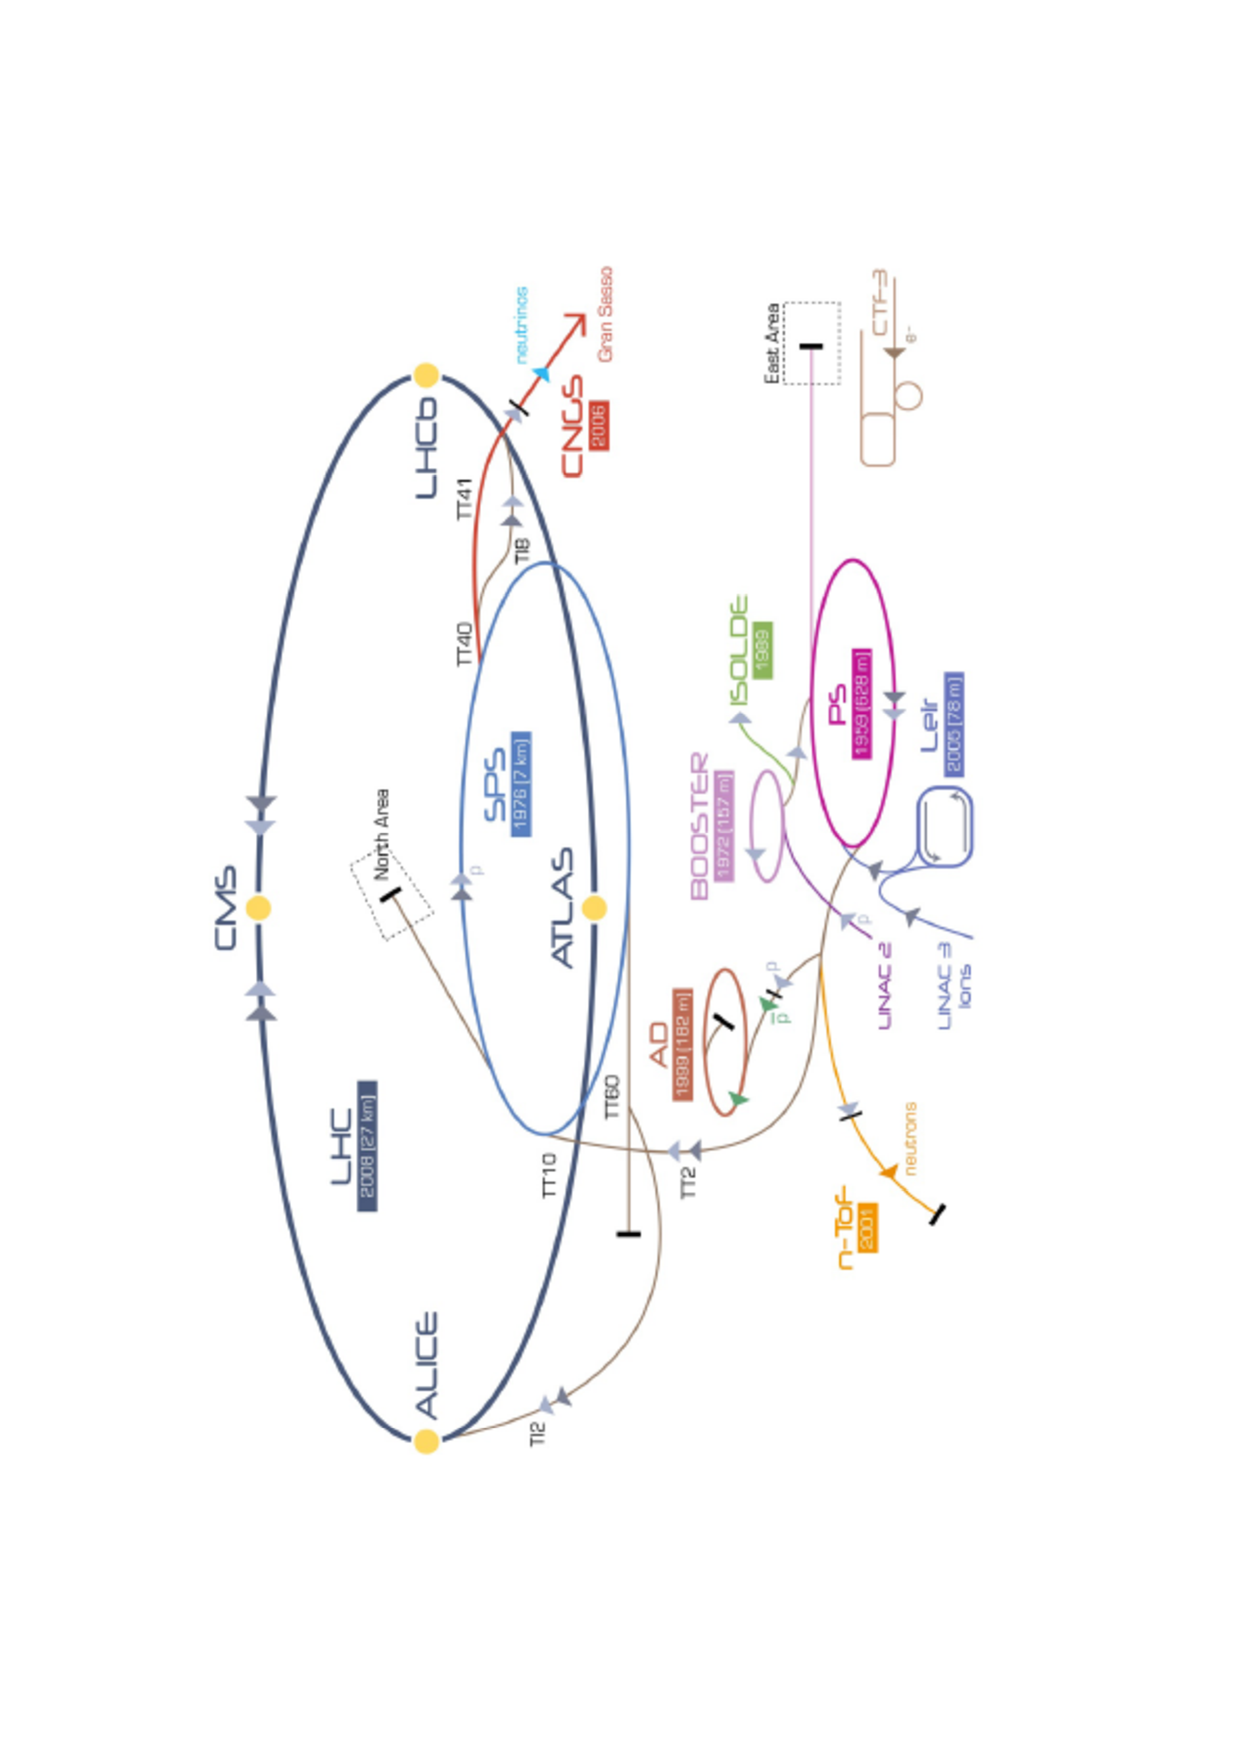
\includegraphics[width=0.70\textwidth,angle=-90]{LHC_ATLAS/CERNaccelerators}
	\caption{Simple sketch of the complex of the accelerators at CERN, from Linac2 to LHC}	
	\label{fig:accelerators}
\end{figure}

As mentioned earlier the LHC accelerator consists in a double ring complex of nearly \SI{27}{\km} lenght. It is made up of 8 arcs containing the dipole bending magnets and 8 long straight accelerating section. The purpose of the magnets, made of superconducting material such as Niobium-titanium or Niobium-tin (\ce{Nb_3Sn}), is to provide to the beam a stable orbit: dipole magnets keep the particles in an almost circular orbit (even when it is bent by the Moon) and quadrupole magnets focus the beam. Magnets are kept at \SI{1.9}{\K} by superfluid helium providing a magnetic field of \SI{8}{\tesla}. Acceleration is provided by radiofrequency resonant cavities which also keep the beam at a constant energy compensating for \mbox{energy} losses and distribute the protons in bunches separated by \SI{25}{\ns} from another. LHC uses 8 cavities per beam each delivering \SI{5}{MV\per\m} at \SI{400}{\MHz} giving the beam \SI{500}{\keV} every turn.
In order to avoid collision between hadrons and gas particles in the tubes, vacuum has to be made in them down to a pressure of \SI{e-13}{atm}.

\begin{table}[tp]
	\centering
	\begin{tabular}{lc}
	\toprule
	Quantity& Value\\
	\midrule
	Circumference& \SI{26659}{\m}\\
	Dipole operating temperature& \SI{1.9}{\K}\\
	Energy, protons& \SI{6.5}{\TeV}\\
	Energy, heavy ions& \SI{2.56}{\TeV\per \amu}\\
	Peak magnetic dipole field& \SI{7.74}{\tesla}\\
	Distance between bunches& $\sim$ \SI{7.5}{\m}\\
	Peak Luminosity (protons)&  \SI{2.06e34}{\per \cm \squared \per \s}\\
	Designed Luminosity (heavy ions)& \SI{e27}{\per \cm \squared \per \s}\\
	No. of bunches per proton beam& 2808\\
	No. of protons per bunch (at start)& \SI{1.2e11}{}\\
	Number of turns per second& \num{11245}\\
	Number of collisions per second& $\sim$\SI{4e7}{}\\
	Frequency of collisions& \SI{40}{\MHz}\\
	Beam width&\SI{17}{\um}\\
	\bottomrule
	\end{tabular}
	\caption{Table listing the main features of LHC}
\end{table}

The LHC was designed to operate with a \cm energy of $\sqrt{s}=\SI{14}{\TeV} $ for protons, even if this energy has not been reached yet, and \SI{1150}{\TeV} (or \SI{5.12}{\TeV\per\amu}) for heavy ions, and a rate of collision of \SI{e34}{\per \cm \squared \per \s}, express in term of instantaneous luminosity. 
At the LHC the insantaneous luminosity is computed with the formula:
\begin{equation}
	\mathcal{L}=\frac{f_{\textup{LHC}} \cdot n_{\textup{b}} \cdot N_{\textup{bunch}}^2}{A}
\end{equation}

where $f_{\textup{LHC}}$ is the collision frequency, $n_{\textup{b}}$ is the number of bunch colliding, $N_{\textup{bunch}}$ is the number of particle per bunch. Finally $A=4\pi\sigma_x\sigma_y$ where $\sigma_k$ are the r.m.s of the distributions of the beams particles along the transverse plane. Instantaneous luminosity can be potentially increased for example by reducing the bunch section or increasing the number of protons per bunch even if it's not very wise for effects discussed later in this section.

With the instantaneous luminosity one can predict the number of events expected in the detector. Since the event rate is given by 
\begin{equation}
\Gamma\equiv\frac{dN}{dt}=\mathcal{L}\times\sigma,
\end{equation}

where $\sigma$ is the total \pp cross section which at $\sqrt{s}=\SI{13}{\TeV}$ is about \SI{80}{mb}. Therefore we expect a rate of about \SI{e9}{events \per\s}, considering a collision rate of \SI{40}{\MHz} we can estimate approximately 25 collisions occurring for each bunch crossing. Along with istantaneous luminosity the integrated luminosity (L) is defined by simply integrating over time the instantaneous luminosity, in formul\ae:
\begin{equation}
	L=\int{\mathcal{L}dt}
\end{equation} 
so that the total number of events can be expressed as:
\begin{equation}
N=L\times\sigma
\end{equation}

The integrated luminosity versus time delivered by LHC, collected by ATLAS and certified to be good for physics during \RunTwo is plotted in \Fig{\ref{fig:lumi}} while a plot of the peak luminosity in stable beam conditions is given in \Fig{\ref{fig:peakLumiByFill}}.
\begin{figure}[tp]
	\centering
	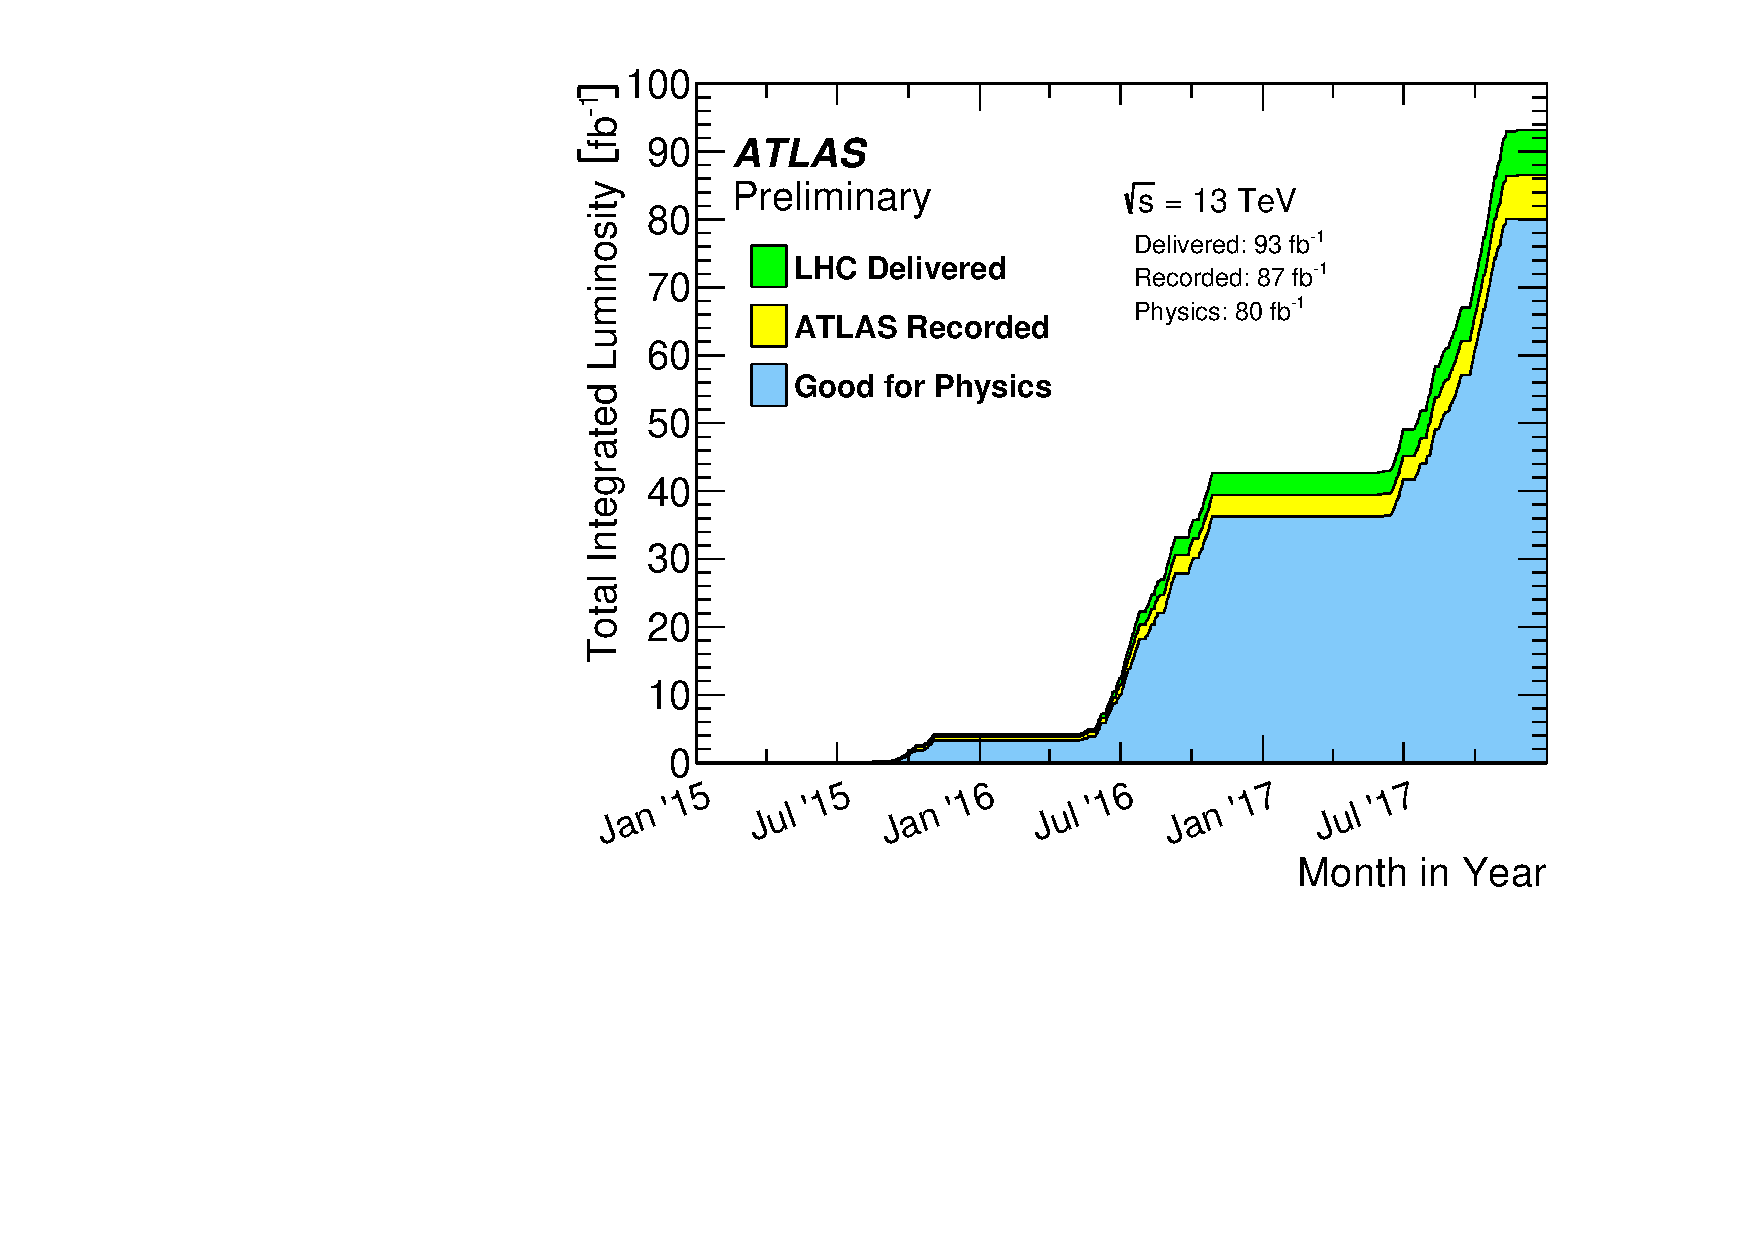
\includegraphics[width=0.75\textwidth]{LHC_ATLAS/intlumivstimeRun2DQ.pdf}
	\caption{Integrated luminosity versus time delivered to ATLAS (green), recorded by ATLAS (yellow), and certified to be good quality data (blue) during stable beams for pp collisions at \SI{13}{TeV} \cm energy in 2015-2017.}
	\label{fig:lumi}
\end{figure}
\begin{figure}[tp]
	\centering
	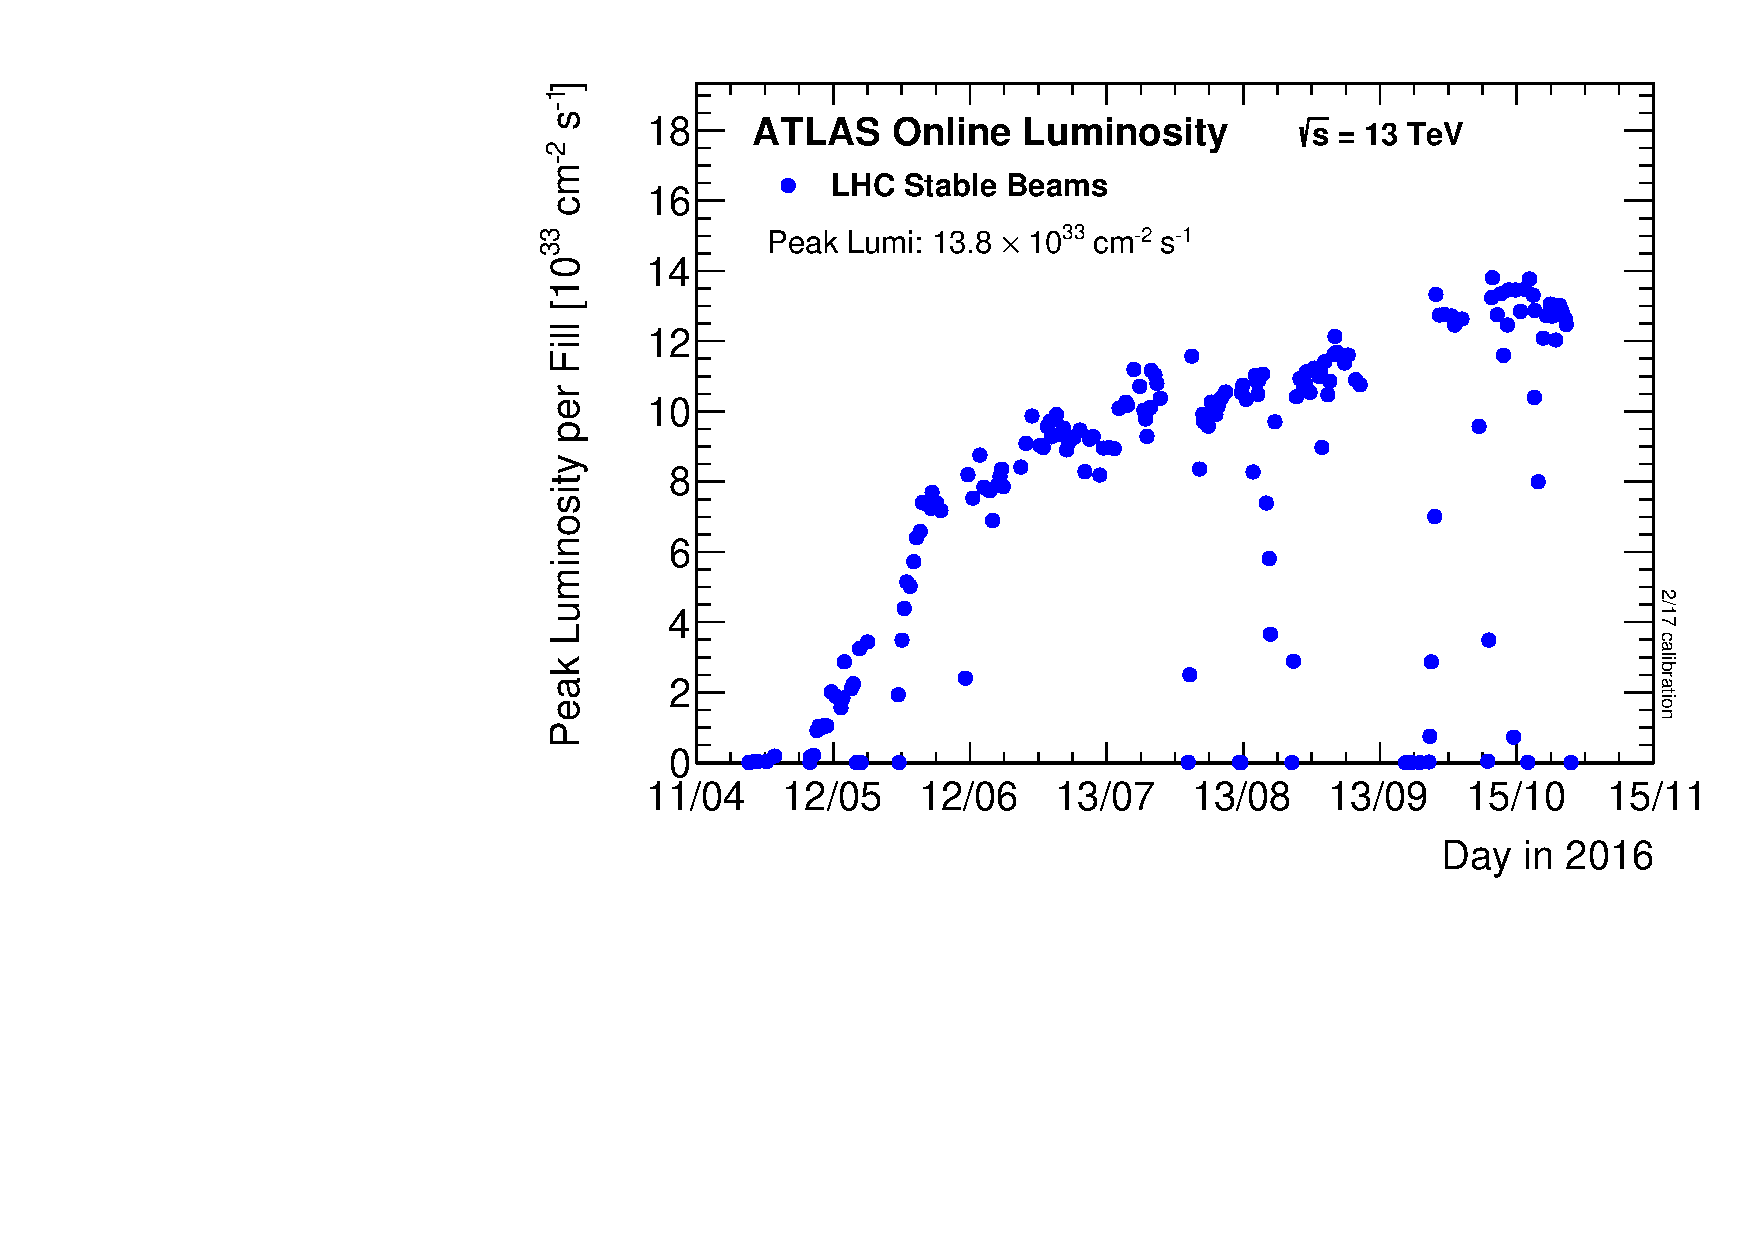
\includegraphics[width=0.75\textwidth]{LHC_ATLAS/peakLumiByFill}
	\caption{Peak instantaneous luminosity delivered to ATLAS during stable beams for pp collisions at 13 TeV centre-of-mass energy for each LHC fill as a function of time in 2016. Designed luminosity of \SI{e34}{\per\cm\squared\per\s} has already been exceded during that year}
	\label{fig:peakLumiByFill}
\end{figure}

Among the events recorded at LHC one can distinguish \emph{soft collisions} and \emph{hard collisions}.
\begin{description}
\item[Soft collisions] These are the most frequent collisions happening between two protons behaving like elementary particle. The momentum transfer is relatively small so that products of the collision scatter for a little polar angle. They have large longitudinal \mbox{momentum}, but small transverse momentum \pt of about \SI{500}{\MeV}.
\item[Hard collisions] Even though they are very rare, they are the most relevant collisions to be taken into account. In this kind of collisions the interaction happens at the quark size. The energy involved in the collision is carried by partons whose momentum which is not known \emph{a priori}, but can be extimated from the Parton Distribution Function (PDF) giving the distributions of quark and gluon momenta inside the proton. From hard scatterings we can produce particles with high \pt with eventually high mass.
\end{description}

What a detector produces is always a superimposition of this two kind of collisions. The principal source of noise in the detector comes from \pileup interactions, i.e. additional \pp collisions that are recorded as belonging to the same event, but are in fact originated by distinct collisions. It can be distinguished in \emph{in time \pileup} when multiple interaction comes from the same bunch crossing and \emph{out of time \pileup} when previous scattering left any electronic signal in the detector which overlap with the one from successive collisions. In order to avoid this unpleasant situation, LHC detectors have been built along a \emph{fast response time} cryterium so they do not integrate signal over many bunch crossings. \textbf{Finally the underlying event must be taken into account, i.e. products from a hard scattering collision but the hard collision itself. They happens between the rest of the partons of the protons which undergo the hard collision. Its product sums up with \pileup either contributing to the background or interact in a way to cover the interesting events}.

\section{The ATLAS detector}
\begin{figure}[tp]
	\centering
	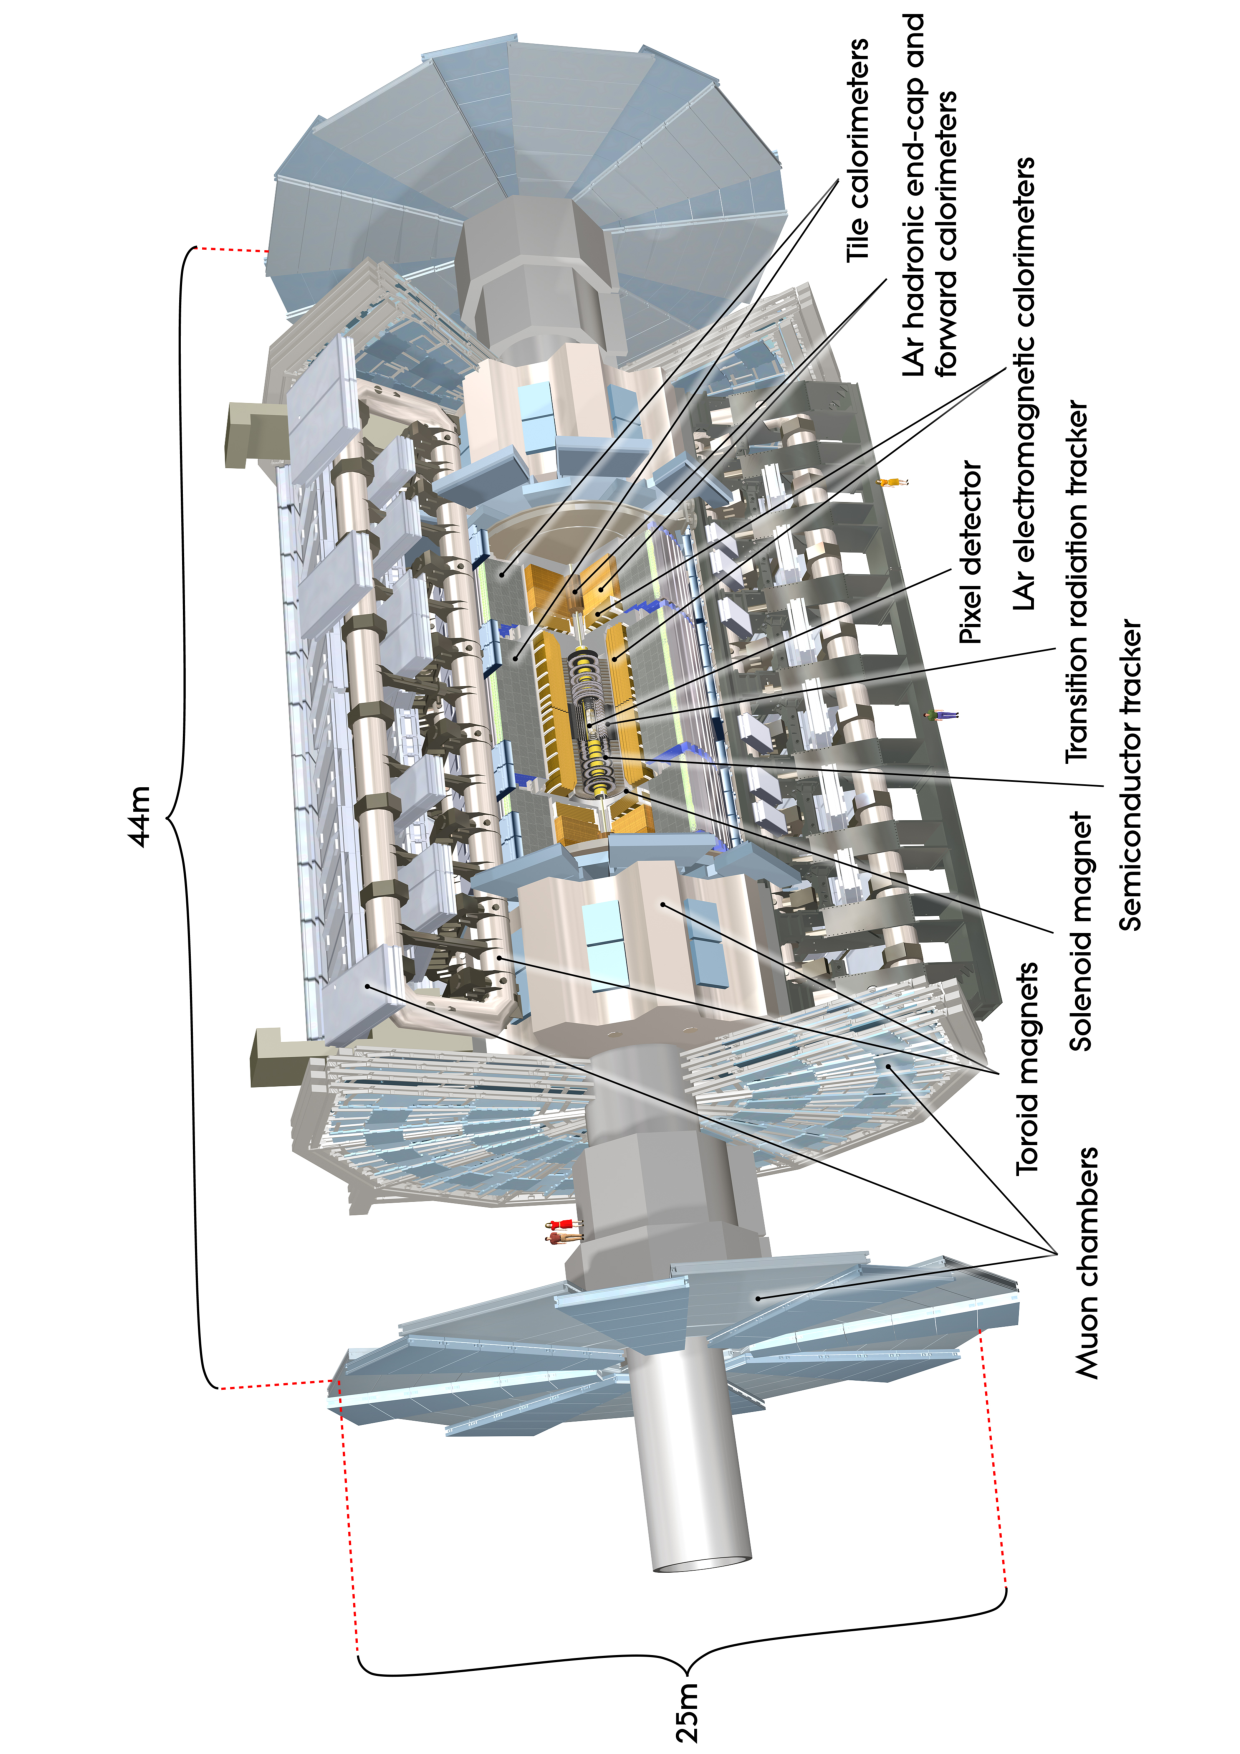
\includegraphics[scale=0.4,angle=-90]{LHC_ATLAS/0803012_01}
	\caption{Cut-away view of the ATLAS detector. The dimensions of the detector are 25 m in height and 44 m in length. The overall weight of the detector is approximately 7000 tonnes.}	
	\label{fig:atlas}
\end{figure}
ATLAS is A Toroidal Large ApparatuS being part of the four most important detectors built around the LHC which are ATLAS, CMS, ALICE and LHCb. ALICE is a detector specialized in measuring and analysing lead-ion collisions, LHCb studies the asymmetry between matter and antimatter in $B-$mesons while CMS and ATLAS are two \emph{general-purpose} experiment aiming to similar goals but with different technical solutions. A greater detailed description of the ATLAS experiment is given in \cite{atcollab:jinst}.

\subsection{Coordinate system}
The frame of reference used in ATLAS is very simple and it considers its origin in the nominal point of interaction. The \emph{z-}axis is defined along the beam direction so that the \emph{x-y} plane is orthogonal to it. The \emph{z} coordinate allows us to define two side of the detector: the \emph{A-side} where \emph{z} is positive and the \emph{C-side} where it's not. In the transverse plane the \emph{x-}axis points towards the center of the LHC ring and the \emph{y-}axis points upwards completing the right-handed triad. In the \emph{x-y} plane, which is the transverse plane, transverse momentum \pt and missing transverse energy \met, along with proper trasverse energy \et can be defined.

Along with carthesian, one can also use polar coordinates to locate objects. The \emph{azimuthal} angle $\phi$ is measured around the beam axis starting from positive \emph{x} and proceeding counterclockwise, while the \emph{polar} angle $\theta$ is defined to be the angle from the beam axis. A simple sketch of the coordinate system used in ATLAS is described in \Fig{\ref{fig:coordinate}}.

It is usually prefered to work with Lorentz-invariant quantities since collisions happen between partons whose boost is unknown. The rapidity $y$ transforms under Lorentz boost via a simple constant addition so that its difference is an invariant quantity. This quantity is used for massive objects like jets, when dealing with ultra-relativistic particle $y$ simplifies into the pseudorapidity $\eta$ which is trivially expressed in terms of the polar angle in the following way:
\begin{gather}
	y=\frac{1}{2}\log{\frac{E+p^z}{E-p^z}}\\
	\eta=-\log{\tan{\frac{\theta}{2}}}
\end{gather}

Distances in this plane are defined as:
\begin{equation}
	\Delta R=\sqrt{\left(\Delta \eta \right)^2 + \left(\Delta \phi \right)^2}
\end{equation}

Cones of constant pseudorapidity for notable value in ATLAS are highlighted in \Fig{\ref{fig:pseudorapidita}}. Pseudorapidity helps also to distinguish various region of the detector: the barrel (central) region which extends up to \AetaRange{1.5}, the  end-cap region \etaRange{1.5}{3.2} and the forward region which covers the \etaRange{3.2}{4.9}

\begin{figure}[tp]
\footnotesize
\centering
	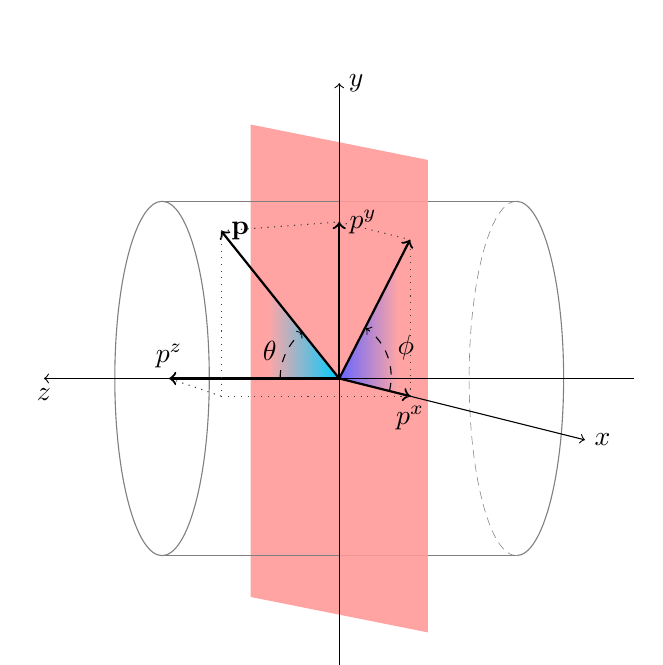
\begin{tikzpicture}[scale=0.75]
	
		\draw[gray] (-2.2,0) arc[x radius = 0.8, y radius = 3, start angle= 0, end angle= 360];
		\draw[gray] (3,3) -- (0,3); \draw[gray] (3,-3) -- (0,-3);
		\draw[gray,very thin,densely dashed] (3,3) arc[x radius = 0.8, y radius = 3, start angle= 90, end angle= 270];
		
		\draw[draw=none,fill=red!40!white,opacity=.9] (-1.5,4.3)--(1.5,3.7)--(1.5,-4.3)--(-1.5,-3.7)--cycle;

		\draw[gray] (3,-3) arc[x radius = 0.8, y radius = 3, start angle= -90, end angle= 90];
  	 	
  	 	\draw[gray] (0,3) -- (-3,3); \draw[gray] (0,-3) -- (-3,-3);
  	 	
  	 	
  	 	\draw[draw=none,  left color= blue!60!white, right color=red!35!white] (0,0)--(1,-0.25) -- (1,1.95) --cycle;
  	 	\draw[draw=none, right color= cyan!80!blue, left color=red!35!white] (0,0)--(-1.2,0) -- ( -1.2,1.53) --cycle;
  	 	\draw[->,dashed] (-1,0) arc [radius=1, start angle=180, end angle= 128] node[left =12pt, below]{$\theta$};
  	 	\draw[->,dashed] (0.85,-0.2125) arc [radius=1, start angle=-14.04, end angle= 55.3] node[below=7pt, right=8pt]{$\phi$};
  	 	
  	 	\draw[->,thick] (0,0)--(-2,2.5) node [right] {$\textbf{p}$};
  	 	\draw[->,thick] (0,0)--(1.2,2.35) node [right] {\textbf{\pt}};
  	 	\draw[->,thick] (0,0)--(-2.88,0) node [above ] {$p^{z}$};
  	 	\draw[->,thick] (0,0)--(1.2,-0.3) node [below ] {$p^{x}$};
  	 	\draw[->,thick] (0,0)--(0,2.65) node [right ] {$p^{y}$};
  	 	
  	 	\draw[thin,dotted,darkgray] (-2,2.5)--(-2,-0.3);
		\draw[thin,dotted,darkgray] (-2,-0.3)--(1.2,-0.3);
		\draw[thin,dotted,darkgray] (1.2,-0.3)--(1.2,2.35);
		\draw[thin,dotted,darkgray] (-2,2.5)--(0,2.65);
		\draw[thin,dotted,darkgray] (0,2.65)--(1.2,2.35);
		\draw[thin,dotted,darkgray] (-2,-0.3)--(-2.88,0);
		

		%===ASSI===
		\draw [->,thin] (5,0)--(-5,0) node[below]{$z$};
		\draw [->,thin] (0,0)--(4.16,-1.04) node[right]{$x$};
		\draw [->,thin] (0,-5)--(0,5) node[right]{$y$};
	
	\end{tikzpicture}
	\caption{Sketch of the frame of reference used in the ATLAS detector which is represented as a simple cilinder. The $z$ axis points along the beam, the $y$ axis points upwars and the $x$ axis points toward the center of LHC ring. The polar angle $\theta$ and the azimuthal angle $\phi$ are represented. The vector $\textbf{p}$ is decomposed in its component $(p^x,p^y,p^z)$ and its transverse part $\textbf{\pt}=p^x \textbf{e}_x+p^y \textbf{e}_y$ lying in the red transverse plane in the middle is pointed out.}
\label{fig:coordinate}
\end{figure}
\begin{figure}
  \centering 
  
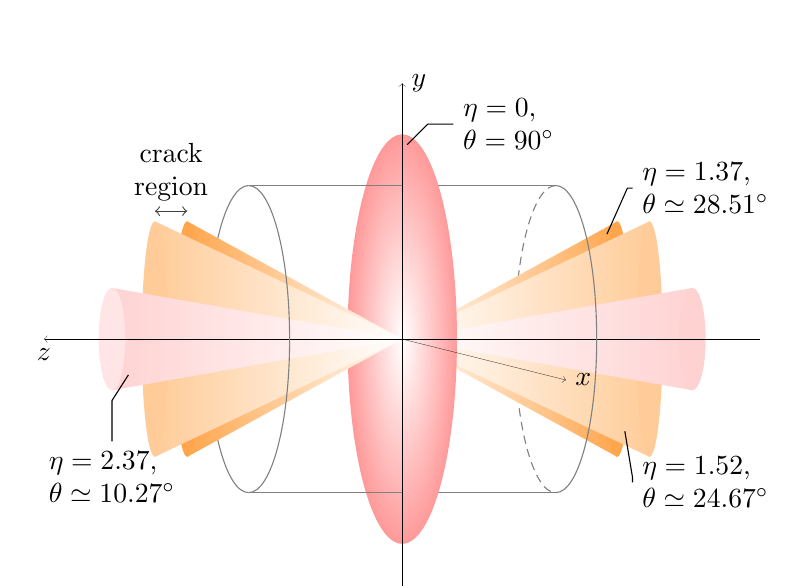
\begin{tikzpicture}[scale=0.65]
	\draw[gray,densely dashed] (3,3) arc[x radius = 0.8, y radius = 3, start angle= 90, end angle= 270];
	\draw[gray] (-3,3) arc[x radius = 0.8, y radius = 3, start angle= 90, end angle= 270];
	\draw[gray] (3,3) -- (0,3); \draw[gray] (3,-3) -- (0,-3);
	
	%eta1.37
	\draw[right color=orange!70!white, left color=white,draw=none] (0,0)--(4.2,2.3)--(4.2,-2.3) --cycle;
	\draw[fill=orange!70!white,draw=none] (4.2,2.3)arc[x radius = 0.26, y radius = 2.3, start angle= 90, end angle= 450];
	\draw[thin] (4,2.05) -- (4.4,2.95) -- (4.5,2.95) node[right,align=left] {$\eta=1.37$, \\$ \theta\simeq\ang{28.51}$};

	%eta1.52
	\draw[right color=orange!40!white, left color=white,draw=none] (0,0)--(4.83,2.3)--(4.83,-2.3) --cycle;
	\draw[fill=orange!40!white,draw=none] (4.83,2.3)arc[x radius = 0.26, y radius = 2.3, start angle= 90, end angle= 450];
	\draw[thin] (4.35,-1.8) -- (4.5,-2.7) -- (4.5,-2.8) node[right,align=left] {$\eta=1.52$, \\$ \theta\simeq\ang{24.67}$};
	
	%eta2.37
	\draw[right color=pink!70!white, left color=white,draw=none] (0,0)--(5.67,1)--(5.67,-1) --cycle;
	\draw[fill=pink!70!white,draw=none] (5.67,1)arc[x radius = 0.26, y radius = 1, start angle= 90, end angle= 450];

	
	%eta0
	\draw[inner color =white, outer color=red!40!white,draw=none] (0,0) ellipse (1.07 and 4);	
	\draw[thin] (0.1,3.8) -- (0.5,4.2) -- (1,4.2) node[right,align=left] {$\eta=0,$ \\$ \theta=\ang{90}$};
	
	%eta1.37left
	\draw[left color=orange!70!white, right color=white,draw=none] (0,0)--(-4.2,2.3)--(-4.2,-2.3) --cycle;
	\draw[fill=orange!70!white,draw=none] (-4.2,2.3)arc[x radius = 0.26, y radius = 2.3, start angle= 90, end angle= 450];
	
	%eta1.52left
	\draw[left color=orange!40!white, right color=white,draw=none] (0,0)--(-4.83,2.3)--(-4.83,-2.3) --cycle;
	\draw[fill=orange!40!white,draw=none] (-4.83,2.3)arc[x radius = 0.26, y radius = 2.3, start angle= 90, end angle= 450];
	
	%eta2.37left
	\draw[left color=pink!70!white, right color=white,draw=none] (0,0)--(-5.67,1)--(-5.67,-1) --cycle;
	\draw[fill=pink!40!white,draw=none] (-5.67,1)arc[x radius = 0.26, y radius = 1, start angle= 90, end angle= 450];
	\draw[thin] (-5.35,-0.7)--(-5.67,-1.2) -- (-5.67,-2) node[below,align=left] {$\eta=2.37$, \\$ \theta\simeq\ang{10.27}$};
	
	\draw[<->,darkgray] (-4.83,2.5)--(-4.2,2.5);
	\draw[] node at (-4.515,2.5) [above,align=center]{crack\\ region};
	%\draw[] node at (7.3,-0.3) [right,align=right]{$\eta=\infty,$\\ $\theta=\ang{0}$};

  	\draw [->,ultra thin] (7,0)--(-7,0) node[below]{$z$};
	\draw [->,ultra thin] (0,0)--(3.2,-0.8) node[right]{$x$};
	\draw [->,ultra thin] (0,-5)--(0,5) node[right]{$y$};
	\draw[gray] (-3,3) arc[x radius = 0.8, y radius = 3, start angle= 90, end angle= -90];
	\draw[gray] (0,3) -- (-3,3); \draw[gray] (0,-3) -- (-3,-3);
	
	\draw[gray] (3,-3) arc[x radius = 0.8, y radius = 3, start angle= -90, end angle= 90];

\end{tikzpicture}
\caption{Notable value of $\eta$ for the corresponding $\theta$. The crack region  for\etaRange{1.37}{1.52}, along with the limit of photon acceptance in this analysis for $\eta = 2.37$  are highlighted. The gray cilinder is a sketch of the ATLAS detector. Due to left-right simmetry, the $\theta$ angle displayed represent both the value shown and their $\pi-\theta$ symmetric. When $\theta$ approaches \SI{0}{°}, $\eta$ assumes larger values. }
\label{fig:pseudorapidita}
 \end{figure}

\subsection{General overview}
ATLAS geometry is mostly driven by three superconducting toroids (one barrel and two end caps). So ATLAS shows a forward/backward symmetry wrt the interaction point and a cilyndrical symmetry around the beam axis. There is also a thin superconducting solenoid surrounding the inner detector (ID), and provides a magnetic fields of about \SI{2}{\tesla}.

The ATLAS detector can be divided into three subdetectors, each one providing a precise task and accomplishing a certain measurement for a specific class of particles. The various part of ATLAS, which will be explained in this section in greater detail, and how particles behave with them is shown in \Fig{\ref{fig:behaviour}}, their coverage in pseudorapidity is given in \Tab{\ref{tab:eta}}.
\begin{description}
\item[Inner Detector] Immersed in the solenoid magnetic field, it provides charged particles momentum measurements and primary and secondary vertices measurements. It is composed of semiconductor pixel, including the Insertable B-layer which was added before the start of \RunTwo, strip detectors in its inner part and straw-tube tracking detectors with the capability to generate and detect transition radiation in its outer part. It will be described in detail in \Sect{\ref{sec:ID}}.
\item[Calorimetry system] It is composed by two kind of calorimeters: a Liquid Argon (LAr) electromagnetic calorimeter and a hadronic calorimeter. They exhibit an excellent energy and position resolution for electrons, photos and jets of hadrons, It covers a very wide range in pseudorapidity for \AetaRange{4.9}. For more detail see \Sect{\ref{sec:calo}}.
\item[Muon spectrometer] The muon spectrometer surrounds the calorimeters. It provides muon momentum measurement which is achieved with three layers of high precision tracking chambers. It includes an air-core toroid system with a long barrel and two side end-caps, which bend muon trajectory. It is described in \Sect{\ref{sec:muons}}.

\begin{figure}[pt]
\centering
\small
\fontfamily{pag}\selectfont
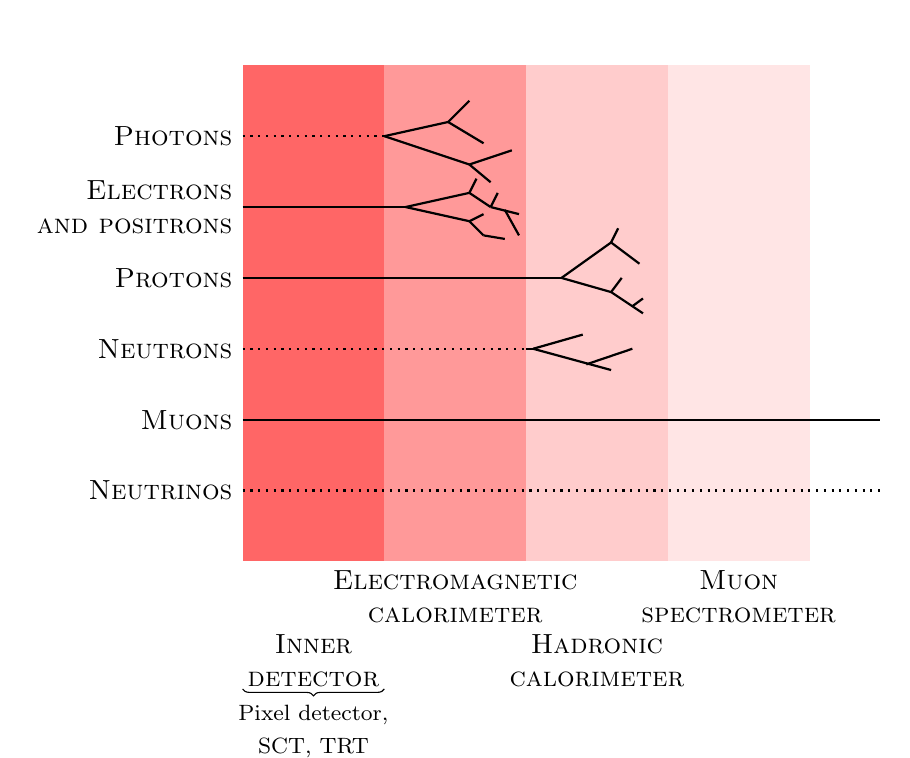
\begin{tikzpicture}[scale=0.9]
	\draw[draw=none,fill=red!60!white] (0,0) rectangle +(2,7);
	\draw[draw=none,fill=red!40!white] (2,0) rectangle +(2,7);
	\draw[draw=none,fill=red!20!white] (4,0) rectangle +(2,7);
	\draw[draw=none,fill=red!10!white] (6,0) rectangle +(2,7);
	
	\draw[thick,dotted] node[left] at (0,6) {\scshape Photons};
		\draw[dotted,thick] (0,6)--(2,6);
		\draw[thick] (2,6)--(2.9,6.2);
			\draw[thick] (2.9,6.2)--(3.2,6.5);
			\draw[thick] (2.9,6.2)--(3.4,5.9);
		\draw[thick] (2,6)--(3.2,5.6);
			\draw[thick] (3.2,5.6)--(3.5,5.35);
			\draw[thick] (3.2,5.6)--(3.8,5.8);
	\draw[thick,dotted] node[left,align=right] at (0,5) {\textsc {Electrons}\\ \textsc{and positrons}} ;
		\draw[thick] (0,5)--(2.3,5);
			\draw[thick] (2.3,5)--(3.2,5.2);
				\draw[thick] (3.2,5.2)--(3.3,5.4);
				\draw[thick] (3.2,5.2)--(3.5,5);
					\draw[thick](3.5,5)--(3.6,5.2);
					\draw[thick](3.5,5)--(3.9,4.9);
						\draw[thick](3.7,4.96)--(3.9,4.6);
			\draw[thick] (2.3,5)--(3.2,4.8);
				\draw[thick] (3.2,4.8) --(3.4,4.9);
				\draw[thick] (3.2,4.8) --(3.4,4.6);
					\draw[thick] (3.4,4.6) -- (3.7,4.55);
	
	\draw[thick,dotted] node[left,align=right] at (0,4) {\textsc{Protons}};
		\draw[thick] (0,4)--(4.5,4);
			\draw[thick] (4.5,4) -- (5.2,4.5);
				\draw[thick] (5.2,4.5)--(5.3,4.7);
				\draw[thick] (5.2,4.5)--(5.6,4.2);
			\draw[thick] (4.5,4) -- (5.2,3.8);
				\draw[thick] (5.2,3.8) -- (5.35,4);
				\draw[thick] (5.2,3.8) -- (5.5,3.6);
					\draw[thick] (5.5,3.6) -- (5.65,3.71);
					\draw[thick] (5.5,3.6) -- (5.65,3.5);
	\draw[thick,dashed] node[left] at (0,3) {\scshape Neutrons};
		\draw[thick,dotted] (0,3)--(4,3);
		\draw[thick] (4,3)--(4.1,3);
			\draw[thick] (4.1,3)--(4.8,3.2);
			\draw[thick] (4.1,3)--(5.2,2.7);
				\draw[thick] (4.85,2.78)--(5.5,3);
	
	\draw[thick] node[left] at (0,2) {\scshape Muons} (0,2) -- (9,2);	
	\draw[thick,dotted] node[left] at (0,1) {\scshape Neutrinos} (0,1) -- (9,1);
	
	\node[align=center] at (1,-1.4) {\scshape Inner\\ \scshape detector};
	\node[align=center] at (3,-.5) {\scshape Electromagnetic\\ \scshape calorimeter};
	\node[align=center] at (5,-1.4) {\scshape Hadronic\\ \scshape calorimeter};
	\node[align=center] at (7,-.5) {\scshape Muon\\ \scshape spectrometer};
	\draw [decorate,decoration={brace}] (2,-1.8)--(0,-1.8);
	\node[align=center] at (1,-2.4) {\footnotesize Pixel detector,\\ \footnotesize SCT, TRT};
\end{tikzpicture}
\caption{Particle behavior inside the various parts of the ATLAS detector, dotted lines are invisible to the various detectors.}
\label{fig:behaviour}
\end{figure}

\begin{table}[tp]
	\centering
	\begin{tabular}{lc}
	\toprule
	Detector & Pseudorapidity range\\
	\midrule
	Inner detector& \AetaRange{2.5}\\
	EM calorimeter barrel& \AetaRange{1.475}\\
	EM calorimeter end-cap, outer weel& \etaRange{1.375}{2.5}\\
	EM calorimeter end-cap, inner weel& \etaRange{2.5}{3.2}\\
	Hadronic tile calorimeter barrel& \AetaRange{1.0}\\
	Hadronic tile calorimeter extended barrel& \etaRange{0.8}{1.7}\\
	Hadronic end-cap calorimeter (HEC)& \etaRange{1.5}{3.2}\\
	Hadronic Forward calorimeter (FCAL)& \etaRange{3.1}{4.9}\\
	Muon spectrometer& \AetaRange{2.7}\\
	\bottomrule
	\end{tabular}
	\caption{Table listing the pseudorapidity range for every part of the ATLAS detector}
	\label{tab:eta}

\end{table}

\end{description}

\subsection{Inner Detector}
\label{sec:ID}
\begin{figure}[tp]
\centering
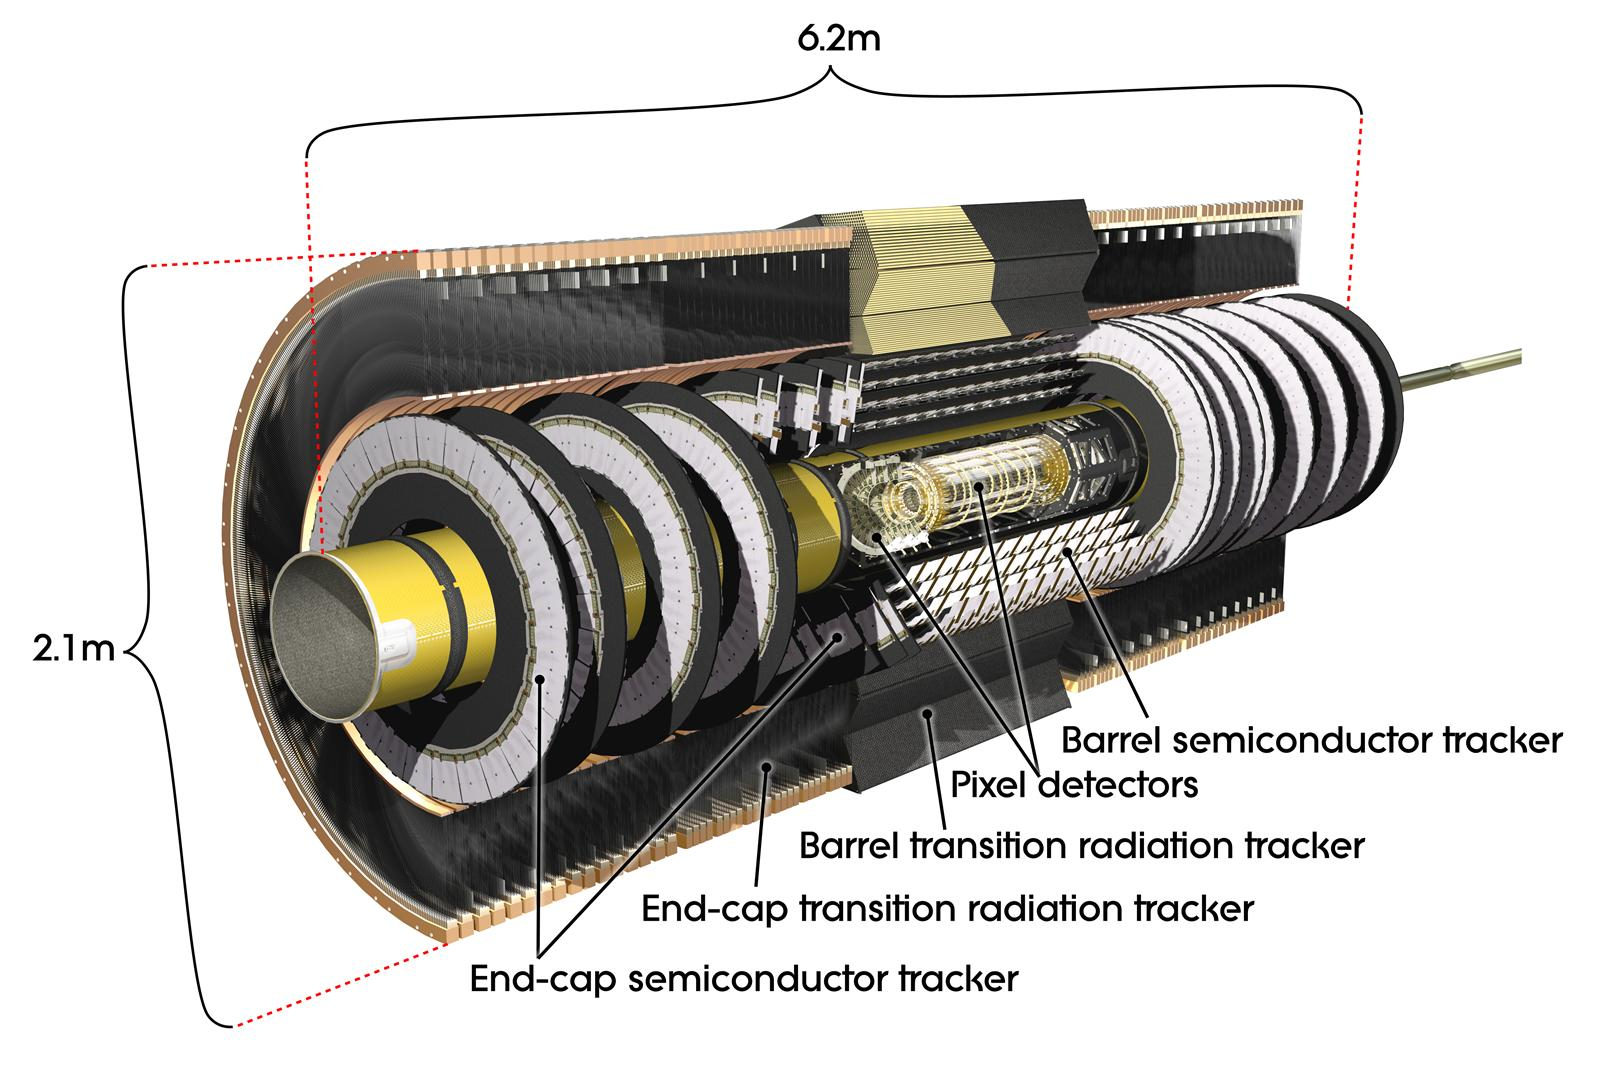
\includegraphics[width=0.8\textwidth]{LHC_ATLAS/ID}
\caption{Cut-away view of the ATLAS inner detector.}
\label{fig:id}
\end{figure}

The Inner Detector (ID), \Fig{\ref{fig:id}}, is a tracking detector and it is designed to provide precise tracks reconstruction, excellent momentum resolution and both primary and secondary vertices measurements. For the purpose of tracking, great precision measurement must be performed so that an high granularity is strongly required. Indeed every \SI{25}{\ns} about \num{1000} particles emerge from the interaction point within a $\eta$ cone of \num{2.5}. Tracking charged particles is very crucial to help other detectors to distinguish between two similar particles. Showers left in the electromagnetic calorimeter by electron and photons are very similar, the only way we have to decide which particle has passed in the detected is looking whether tracks were left in the front of the calorimeter.

\begin{figure}[pt]
\centering
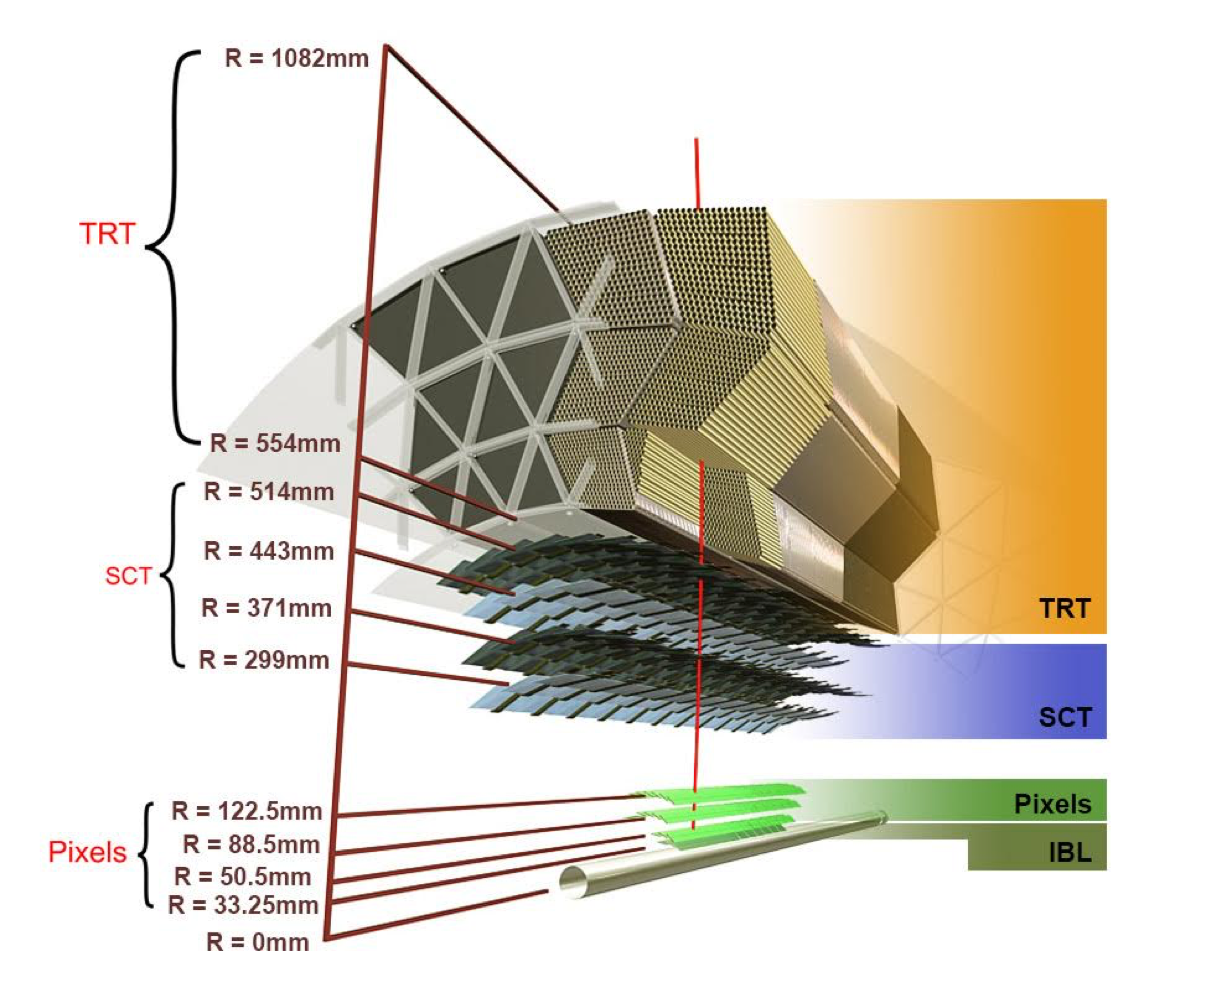
\includegraphics[width=0.8\textwidth]{LHC_ATLAS/IDCrossSection}
\caption{Cross section of the inner detector.}
\label{fig:xsecID}
\end{figure}

The ID is contained within a cylindrical region of radius \SI{1.05}{\m} and lenght \SI{6.2}{\m}. It is immersed in a \SI{2}{\tesla} solenoidal magnetic field and it consists of three independent and complementary parts, as pictured in \Fig{\ref{fig:xsecID}}, which are the Pixel Detector, SemiConductor Tracker (SCT) and the Transition Radiation Tracker (TRT).

The Pixel Detector, covering the \AetaRange{2.5} range, is the closest detector to the beam reaching about \SI{33.25}{\mm} in distance with the Insertable B-layer (IBL) added during LS1. In the barrel region, pixel sensors are arranged on three concentric cylinders around the beam axis while in the end-cap regions they are organized in disks perpendicular to the beam axis. A Pixel sensor is a \si{16.4} $\times$ \SI{60.8}{\mm} wafer of silicon with \num{46080} pixels with a size in $R$-$\phi \times z$ of  \si{50} $\times$ \SI{400}{\um\squared} each. Thanks to its triple layer, the detector provides three measurement points to reconstruct the track with a resolution of \SI{10}{\um} in the direction orthogonal to its disposition and \SI{115}{\um} in the longitudinal one. The pixel detector has approximately \num{92} million readout channels overall.

The SCT is devoted to reconstruct particles momenta. It covers a $R$ distance between \SI{299}{\mm} and \SI{514}{\mm}  from the beam pipe and it consists of modules of silicon strips arranged in four concentric barrels and two end-caps of nine disks each. In the barrel it uses small angle stereo strips to measure a particle's coordinate, with a particular set parallel to the beam axis for measuring $R$ and $\phi$, while in the end-cap it uses a set of strips running radially. 
{\bfseries To get a measure of the $z$ coordinate in the barrel a set of stereo strips at an angle of \SI{40}{mrad} overlaps the one underneath which is kept parallel to the $z$ axis.}
Here eight strip layers corresponding to four space points are crossed by each track. The total number of readout channels in the SCT is approximately 6.3 million, each of them providing a precision of \SI{17}{\um} in the $R$-$\phi$ plane and \SI{180}{\um} in $z$ direction for barrel and in $R$ direction for the end-cap region.

The outer part of the ID is a TRT which occupies a cilinder of radii \SI{554}{\mm} and \SI{1082}{\mm}. The detecting elements are drift tubes (straws) with a diameter of \SI{4}{mm} and \SI{144}{cm} long in the barrel region, where they are parallel to the beam axis being cut in a half at $\eta =0$, and \SI{37}{\cm} long in the end-cap region where they are distributed radially. It provides information only on $R$-$\phi$ coordinates with a resolution of  only \SI{200}{\um} per straw, much less than the other two detectors. On the other hand it provides a very large number of hits per track, which is about \num{36}. The TRT has about \num{298000} straws in total. {\bfseries Its tecnology is based on transition radiation which occurs whenever a charged particle crosses two media with different refractive index. Tracks left, for instance, by electrons and charged pions is very similar. In order to distinguish them one can build this system so that a radiation is emitted only when an electron crosses a straw.}

The combination of precision trackers in the innermost shell with the TRT at a larger radius gives very robust pattern recognition and high precision measurements. For instance the TRT's straws hit at large radius contributes significantly to determine a particle's momentum by compensating their small precision with longer measured track and larger number of hits.

Finally the ID typical momentum resolution is $\frac{\sigma_{\pt}}{\pt}=0.05\%\pt\oplus1\%$.

The Inner Detector system provides tracking measurements in a range matched by the precision measurements of the electromagnetic calorimeter which will be described in the next section.

\subsection{Calorimetry}
\label{sec:calo}
Calorimeters are the detectors dedicated to energy measurements for both neutral an chrged particles, except for muons. To improve the precision of the missing transverse momentum (\met) the pseudorapidity range extends up tp $\eta=4.9$, with a full $\phi$ coverage. Nevertheless there is a blind zone in \etaRange{1.37}{1.52} called \emph{crack region} where the barrel/end-cap transition happens.

In ATLAS the calorimetry system, represented in \Fig{\ref{fig:Calos}}, is composed by two subsystems: the electromagnetic (EM) calorimeter, optimized to measure photons and electrons thanks to its finer granularity, and the hadronic calorimeter which measure the energy and position of jets of hadrons. Both of them are sampling calorimeters, which means they are made of a series of active and absorber material samples.

An important feature in building them is the calorimeter depth. They must provide good containment for electromagnetic and hadronic showers limiting the amount of electrons, photons and hadrons leaking into the muon spectrometer.

\begin{figure}[tp]
\centering
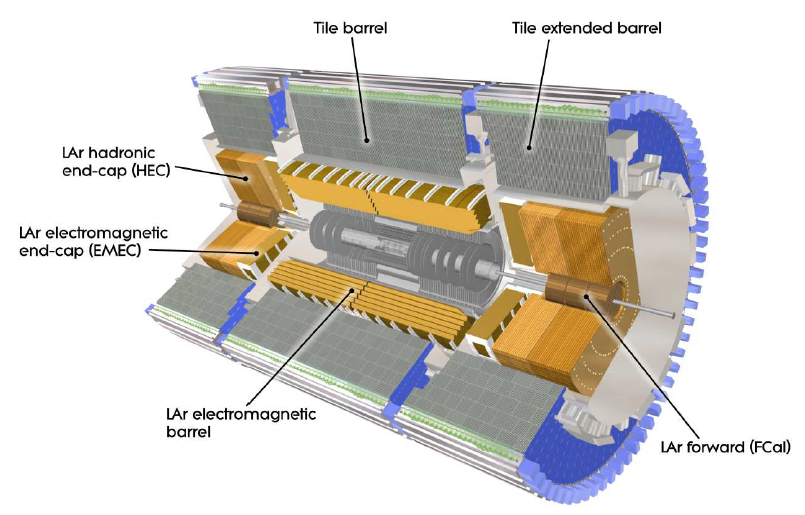
\includegraphics[width=0.8\textwidth]{LHC_ATLAS/Calorimetry}
\caption{Cut-away view of ATLAS calorimetry system. It develops around the inner detector in gray and it is composed by the electromagnetic and hadronic calorimers.}
\label{fig:Calos}
\end{figure}

\subsubsection{Electromagnetic Calorimeter}
\begin{figure}[tp]
\centering
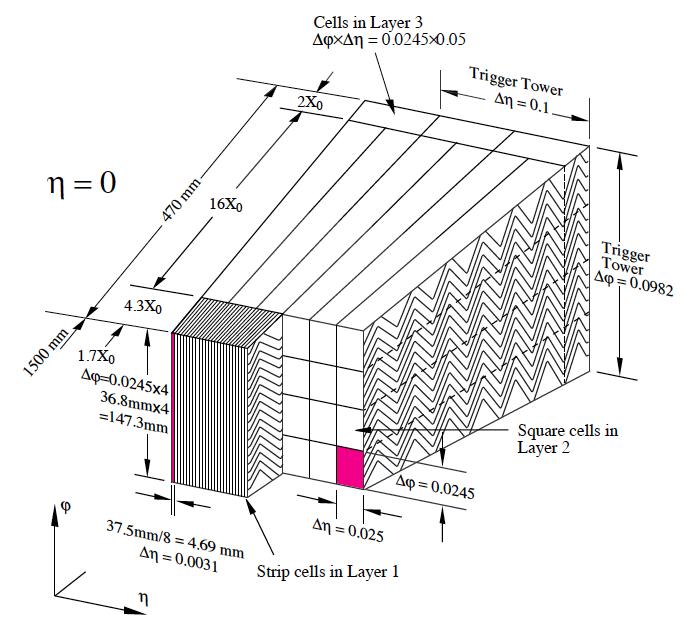
\includegraphics[width=0.55\textwidth]{LHC_ATLAS/EMcalo}
\caption{Schematic view of a fraction of the EM calorimeter showing its accordion geometry and pointing out the segmentation in ``strips'', ``middle'' and ``back'', along with their granularity, in the  barrel region.}
\label{fig:EMlayers}
\end{figure}

The EM calorimeter is designed to detect, measure and track electrons and photons and it is part of the LAr calorimetry. Indeed it adopts entirely this tecnology consisting in a Liquid Argon ionization chamber using lead as absorber. It is composed by two half-barrels, separated at $\eta=0$ by a \SI{4}{\mm} gap, covering \AetaRange{1.475}. Two end-caps (EMEC), composed by a outer and an inner weel, cover the range in pseudorapidity respectively to \etaRange{1.375}{2.5} and \etaRange{2.5}{3.2} each housed in its own cryostat. 

It is built following an accordion geometry which naturally guarantee a full $\phi$ coverage without any cracks. In the barrel the accordion waves are parallel to the beam axis, running in $\phi$, and their folding angle varies with $R$ keeping the LAr gaps pretty constant. In the endcaps, the waves run axially and the folding angle varies with radius.

In the longitudinal direction and for \AetaRange{2.5}, where precise measurements take place, the EM barrel calorimeter is segmented into three longitudinal sections while the inner wheel, for $\abs\eta>2.5$, in two sections. In barrel the three sections are called ``strips'', ``middle'' and ``back'' as shown in \Fig{\ref{fig:EMlayers}}. The strips layer has the highest granularity which reaches \mbox{$0.008 \times 0.1 \left(\Delta \eta \times \Delta \phi \right)$}, needed to distinguish between a decayed \pizero from a real photon. The middle calorimeter layer collects the largest fraction of the energy of eth electromagnetic showers and the back detects their tails and prevents the shower to reach the outer hadronic calorimeter. The total thickness of the EM calorimeter is greater than 22 radiation lengths ($X_0$), which is defined as the mean distance over which a high energy electron loses $1/e$ of its energy by bremsstrahlung, in the barrel and greater than 24 $X_0$ in the end-caps.
  
Going through the ID, energy loss for photons and electrons might happen and it must be taken into account. A presampler, which is a very thin Liquid-Argon layer ($\sim \SI{11}{\mm}$), is added before the calorimeter to recover this kind of energy loss.

\subsubsection{Hadronic Calorimeter}
The Hadronic Calorimeter is characterized by three parts: the tile calorimeter in the barrel region for \AetaRange{1.7}, the LAr hadronic forward (FCal) in the \etaRange{1.4}{3.2} region, and end-cap (HEC) calorimeter for \etaRange{3.2}{4.9}. 

The Tile Calorimeter, placed just outside the EM calorimeter in the radial direction, is a sampling calorimeter which uses steel as absorber and a scintillator as an active medium. It can be divided in the proper barrel region and two extended barrels, both extending from an inner radius of \SI{2.28}{\m} to an outer one of \SI{4.25}{\m} and segmented in depth in three layers. The barrel covers the region \AetaRange{1.0} and the two extended barrels extend the covering to $\eta=1.7$. While speaking of hadrons, the interaction lenghts ($\lambda$), i.e. the mean distance between two hadron-nuclear matter interaction, is used instead of radiation lenght to define the depth of the calorimeter. The interaction lenght can be computed as $\lambda \simeq \frac{A^{1/3}}{\rho}$ where $A$ is the mass number for a specific atom and $\rho$ is the nuclear density. The total detector thickness in the tile-instrumented region is \SI{9.7}{\lambda} at $\eta = 0$ and \SI{10}{\lambda} in the extended barrel.

The HEC and FCal parts use the same technology as in the EM calorimeter so that their active medium is Liquid Argon but their absorber can be tungsten or copper. The HEC is located directly behind the EM end-cap calorimeter, sharing the same cryostat, and it consists of two independent wheels per end-cap. Each weel is divided into two segments in depth, for a total of four layers per end-cap. The FCal completes the $\eta$ coverage of the calorimeter system being located in \etaRange{3.2}{4.9}. It consists of three modules in each end-cap: the first, made of copper, is suited for electromagnetic measurements, while the other two, made of tungsten, measure the energy of hadronic interactions.

\subsection{Muon Spectrometer}
\label{sec:muons}
The Muon Spectrometer is the outermost detector in ATLAS which is shown in \Fig{\ref{fig:muons}}. Its functioning is based on the magnetic deflection of muons in the large superconducting air-core toroid magnets built in such a way the magnetic field is almost orthogonal to muons path. For \AetaRange{1.4} bending is achieved thanks to the barrel toroids, for \etaRange{1.6}{2.7} muons are bent by two smaller end-cap toroids and in the intermediate, or transition region (\etaRange{1.4}{1.6}) the deflection occurs from a combination of the two fields. Bending power is computed by the field integral $\int B_{\bot}\,dl$ where $B_{\bot}$ is the field perpendicular to the muons trajectory and the integral is evaluated along the infinitesimal path covered by muons inside the spectrometer. The barrel toroid provides \SI{1.5}{\tesla \metre} to \SI{5.5}{\tesla \metre} and the end-cap toroid gives from \SI{1}{\tesla \metre} to \SI{7.5}{\tesla \metre}. The magnetic field is continuously monitored by almost 1800 Hall sensors distributed throughout the spectrometer: this is crucial in order to calculate the bending power along the muon trajectory to a few parts in a thousand.

In the barrel region, tracks are measured in chambers arranged in three cylindrical layers around the beam axis while in transition and end-cap region three-layered chambers are located in planes orthogonal to the $z$-axis. The tracking chamber are made of Monitored Drift Tube (MDT) which pursue high-precision tracking along almost the whole $\eta$ range. They are made of cylindrical aluminum drift tube being filled with gas which gets ionized when a muon passes by. Charge is collected by a wire held at high potential. Cathode-strip chambers (CSC) covers \etaRange{2}{2.7}. They are multiwire proportional chambers with cathodes segmented into strips with an higher rate capability and high granularity.     

The muon spectrometer has its own trigger system which extends over \AetaRange{2.4} and uses Resistive Plate Chambers (RPC) and Thin-gap Chambers (TGC) in barrel and end-cap regions respectively.{\bfseries Its typical momentum resolution $\frac{\sigma_{\pt}}{\pt}$ varies from 2\% to 5\% in the range between \SI{1}{\TeV} and \SI{10}{\TeV}.}

\begin{figure}[pt]
\centering
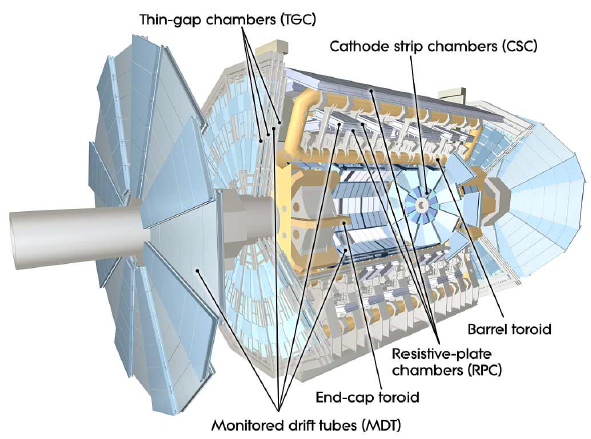
\includegraphics[width=0.7\textwidth]{LHC_ATLAS/Muons}
\caption{Cut-away view of the ATLAS muon system.}
\label{fig:muons}
\end{figure}

\subsection{Forward Detectors}
Three smaller detector systems cover the ATLAS forward region. LUCID (LUminosity measurement using Cerenkov Integrating Detector) at \SI{\pm 17}{\m}, along the beam, and ALFA (Absolute Luminosity For ATLAS) located at \SI{\pm 240}{\m} are used to measure the istantaneous luminosity delivered to ATLAS. The third system is the Zero-Degree Calorimeter (ZDC), located at \SI{\pm 140}{\m}, which is used in determining the centrality of heavy-ion collisions.

\subsection{Trigger system}
The rate of events expected rate at the LHC designed luminosity is \SI{1}{\GHz}, as mentioned in the previous Section, on the other hand the maximum event rate that ATLAS can record is \SI{\sim 1000}{\Hz}. It is evident that an appropriate trigger system must be used so that only events that could have potential physical interest would be recorded. There are two distinct levels of trigger: L1 and the Event Filter. Each trigger level refines the decisions made at the previous level using more refined quantities at each step, and, where necessary, applies additional selection criteria.

L1 looks for high-\pt particles such as electrons, photons, $\tau$-leptons decaying into hadrons as well as large \met and defines one or more Region-of-Interest (RoI) which is a $\Delta \eta \times \Delta \phi$ region in which interesting events can be found. It uses information coming from a subset of detectors which are processed by the central trigger processor. The operating time is about \SI{2.5}{\um} which reduces the event rate down to \SI{100}{\kHz}.

The final stage of the selection is made by the Event Filter (EF) which reduces the rate to a reasonable \SI{1}{\kHz}. It selects events using the full granularity avaliable for each subdetector, and store them as raw data (RDO) for offline analysis. Every event is computed in about \SI{4}{\s}. Performance of L1 and High Level Trigger are show respectively in \Fig{\ref{fig:L1}} and \Fig{\ref{fig:HLT}}.

\begin{figure}[t]
\centering
\subfloat[][L1 performance]
{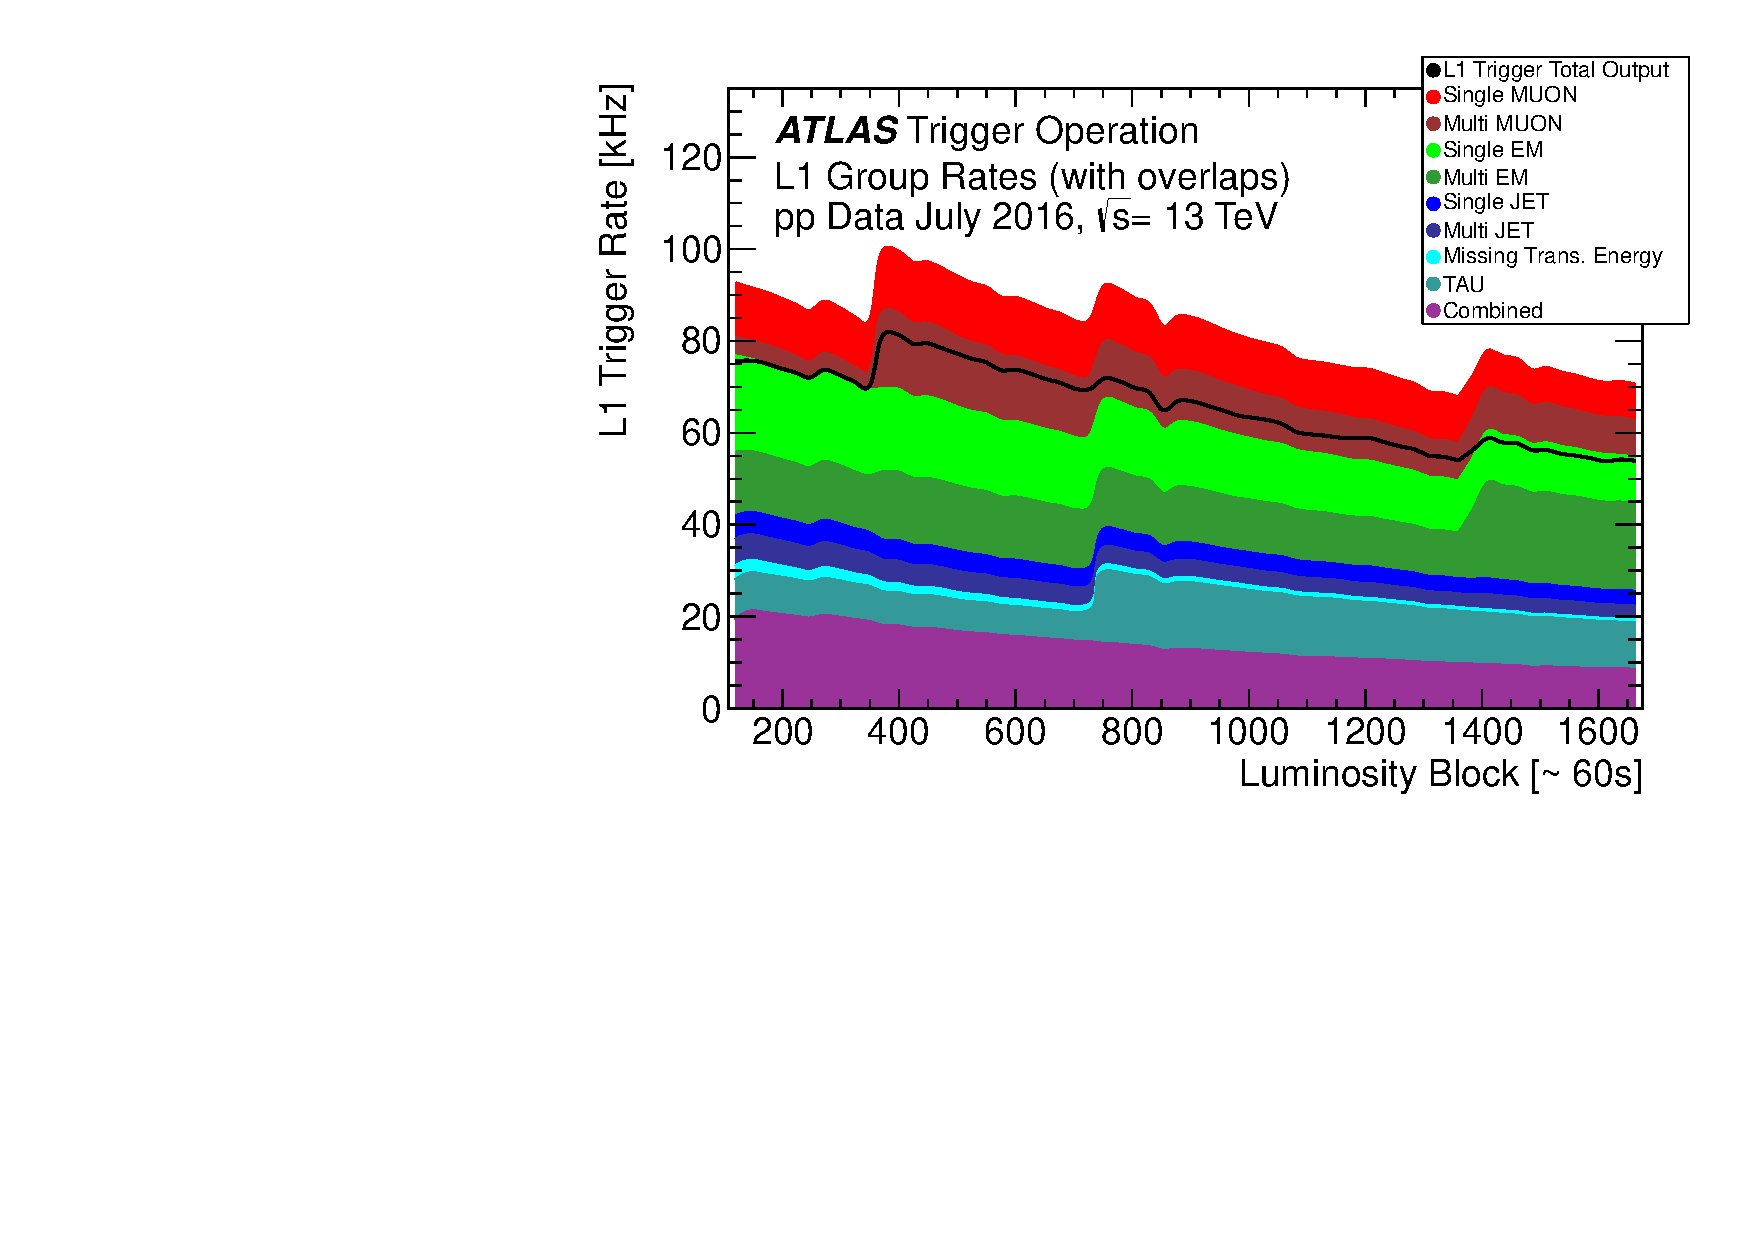
\includegraphics[width=.55\textwidth]{LHC_ATLAS/Time_L1GroupRate_Stack_2016_07} \label{fig:L1}} \\

\subfloat[][HLT performance]
{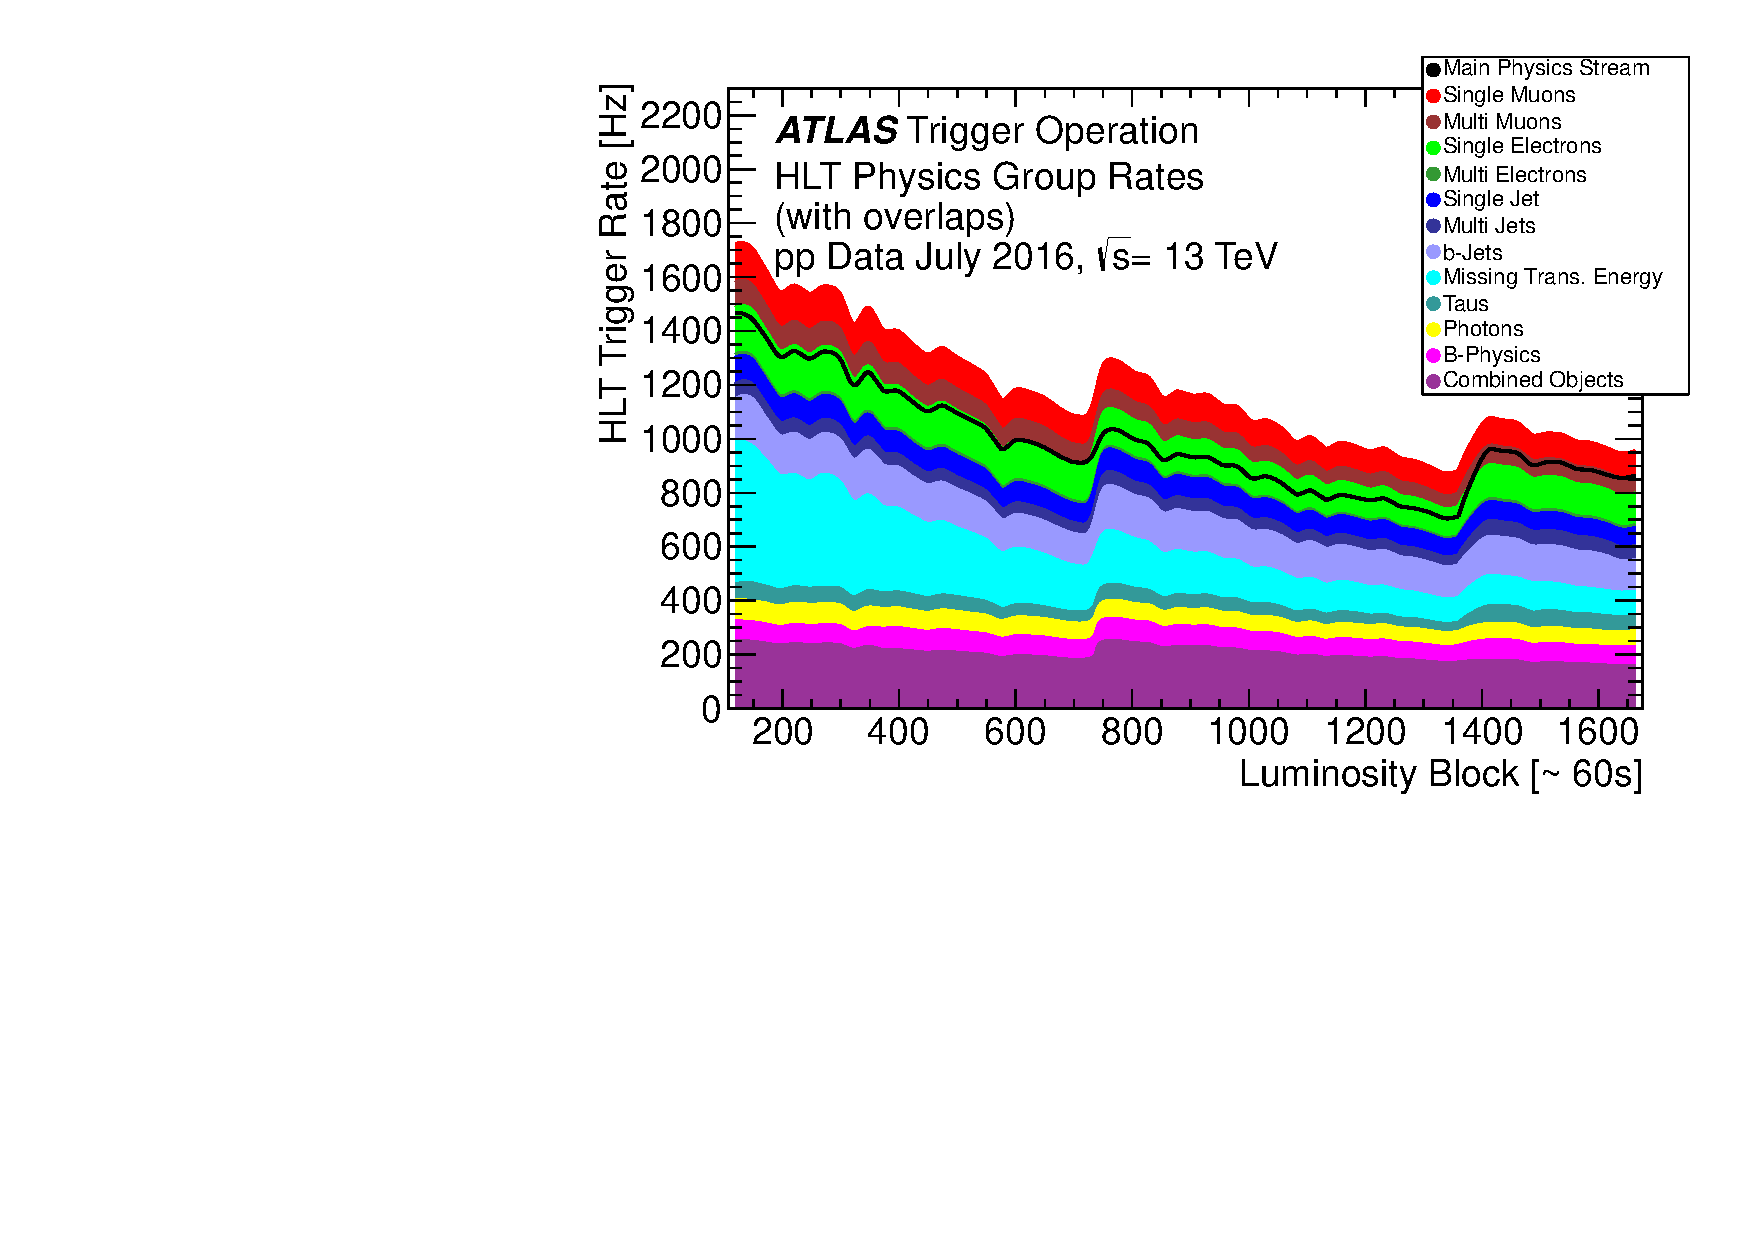
\includegraphics[width=.55\textwidth]{LHC_ATLAS/Time_HLTGroupRate_Stack_2016_07} \label{fig:HLT}}

\caption{Physics trigger group rates at the High Level Trigger (HLT) and the first trigger level (L1) as a function of the number of luminosity blocks which correspond to on average \SI{60}{\s} per luminosity block in a fill taken in July 2016 with a peak luminosity of L = \SI{1.02 e34}{\per\cm\squared\per\s}. We can notice the sawthoot behavior given by loosing of trigger requirements while the beam gets less perfect.}
\end{figure}






\clearpage
\thispagestyle{empty}
\chapter{Dark Matter}
\lettrine{O}{}ne of the most challenging question of modern physics is the nature of Dark Matter (DM). Several evidences discussed in this chapter proves that in the Universe there should be non-luminous matter and most of it is of non-baryonic nature. Currently data proves that ordinary matter should accounts for about \SI{4.56}{\percent}, while Dark Matter accounts for \SI{22.7}{\percent} and Dark Energy for the remaining \SI{72.8}{\percent}.

Dark Matter would constitute the principal non-baryonic contribution to the matter density of the universe. An appealing hypothesis on the Dark Matter nature of is that of the weakly interacting mass particles (WIMPs) which can be produced at collider such LHC if they interact with Standard Model (SM) particles via couplings at the electroweak scale. On the other hand they certainly be detected but their interaction with the detector can be inferred as ``missing momentum'' signature. 

\section{The Standard Model of particle physics}
The Standard Model (SM) of particle physics is a well established theory of elementary particles and their interaction. Up to now it is considered the most satisfying theory including three of the four fundamental forces.
Particles of the SM can be divided into three cathegories. The first comprehend spin \num{1/2} fermions divided in three generations which are the electron, the muon and the $\tau$-lepton with their corresponding neutrinos, along with six flavoured quarks (up, down, strange, charm, top, bottom). The second cathegory includes spin 0 gauge bosons, the force carriers. They are the photon, mediator of electromagnetic force, the \Zboson and \Wboson bosons mediators of weak force and 8 gluons which carry strong interation. At last there is the Higgs Boson, whose existence has been proved with \RunOne ATLAS and CMS data which is responsible 

On the other hand, the SM presents a series of open issues. In addition to major problems such the gauge hierarchy problem, i.e. understand why the Higgs mass is so small compared to the Planck mass, the SM does not contemplate gravitation as a quantum theory nor it provides a particle to be a solid candidate for Dark Matter. There are several extensions of the SM trying to include several neutral, stable or at least long lived, and non-baryonic particles that could explain the nature of DM.

The principal candidate is the so called Weakly Interactive Mass Particle (WIMP). The WIMPs are the most studied Dark Matter candidates, since they would naturally exhibit the relic density from the Big-Bang that we infer from cosmological observations~\cite{feng:DM}.

Before talking about WIMPs, let's introduce several evidences that justify the \mbox{search for DM}.

\section{Physical evidences of Dark Matter}
In this section different astronomical observations that support the idea for non-luminous matter in the Universe are pointed out. The gravitational lensing will be presented first, then the rotation curve of stars in galaxies will be discussed togheter with the Cosmic Microwave Background (CMB) measurements.

\subsection{Gravitational lensing}
Gravitational lensing is the phenomenon for which a very massive object could act as a lens deviating rays of lights. According to general relativity light is affected by the gravitational field produced by massive objects so that a ray of light could be deflected of an angle 
\begin{equation}
\abs{\delta\phi}=\frac{4M}{r}
\end{equation}
Where $\,M$ is the mass of the object producing the field (i.e. the lens), and r is the distance between the photon and the lens. Note that we are using a natural system unit in which $G=1$ and $c=1$.

If the light being deflected comes from an object aligned with the lens and the observer and the lens is pefectly homogeneous, the image produced is a perfect circle, like the Einstein ring shown in \Fig{\ref{fig:einsteinring}}, since light is deflected equally in every direction. What actually happens is a discrete pattern of images around the lens.

The mass of the lens can be approximately evaluated from the deflection angle given the distance of the image from the lens and it accounts for the \emph{total} mass of the lens, i.e. coming from both regular matter and Dark Matter. While calculating it from the lens luminosity Dark Matter contribution is missed.

\begin{figure}[pt]
\centering
\includegraphics[width=0.5\textwidth]{DarkMatter/einsteinring}
\caption{Image of light deflected by a gravitational lens producing an almost perfect Einstein ring}
\label{fig:einsteinring}
\end{figure}

%The model used to predict mass for a lens is the singular isothermal sphere (SIS) \cite{book:971430} which approximates the lens as a spherical ideal gas cloud with constant temperature $T$ for every point in the lens. Defining the density of the lens as $\rho(r)=\sigma_v^2/2\pi G r^2$, where $\sigma_v^2$ is the velocity distribution of the lens components along the line-of-sight, the mass within a sphere of radius $r$ is therefore computed as:
%\begin{equation}
%M(<r)=\int_0^r{\rho(r')4\pi r'^2 dr'}=\frac{2\sigma_v^2}{G}r
%\label{mass}
%\end{equation}

%It is clear that the SIS model is not perfect because, according to \Eqn{\ref{mass}} it gives an infinite total mass, even if it is exploited a lot thanks to its simplicity and its perfect reconstruction of rotation curves of spiral galaxies (\Sect{\ref{sec:rotcurves}}), but further results lie outside of the purpose of this work.

%What we want to point out is that  \Eqn{\ref{mass}} accounts for the \emph{total} mass composing the lens, including both luminous and dark. The latter is missed when we try to calculate it from the luminosity of the lens.
   
\subsection{Rotation curves of stars in a galaxy}
\label{sec:rotcurves}
The study of the rotation curves of galaxies focuses on spiral galaxies which are bound system where stars are not distributed spherically but in a thin disk. Stars up to a radius $r$ from the center of a galaxy are influenced by the total matter contained in a sphere of radius r. At equilibrium centripetal force must be equal to the gravitational attractive force.
\begin{equation}
\frac{mv^2}{r}=\frac{GM(r)m}{r^2}
\label{previous}
\end{equation}
where $M(r)$ is the mass of the galaxy inside a radius $r$ and $m$ is the mass of a single star. From the previous equation one obtains the relation between velocity, mass and radius:
\begin{equation}
v=\sqrt{\frac{GM(r)}{r}}.
\end{equation}

According to the visible mass distribution, the velocity should decrease with radius, but actual measurements show that it remains constant after \SI{\sim5}{pc} as pointed out in data shown in \Fig{\ref{fig:rotation}}. A simple explanation to this behaviour is the presence of a Dark Matter halo throughout the galaxy whose mass distribution is proportional to the distance from the center so that the velocity would be constant.
\begin{figure}[pt]
\centering
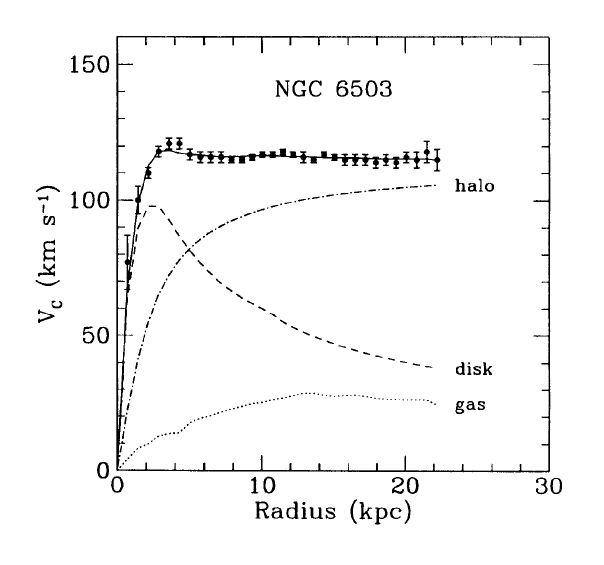
\includegraphics[width=0.4\textwidth]{DarkMatter/Rotationcurves}
\caption{Rotation curves of NGC 6503 galaxy. The image represents a fit on the rotation curves made of three parameters: a stellar (dashed) and a gaseous disk (dotted) and a Dark Matter halo (dash-dotted).}
\label{fig:rotation}
\end{figure}


\subsection{Cosmic Microwave Background}
The CMB is the residue of the thermal microwave radiation emitted \SI{\sim 3e5} years after the Big Bang, when the Universe became transparent to photons. Before that, the Universe was an ionized plasma in which matter and radiation were tightly coupled. It is a relic thermal radiation background which permeate the Universe and it is quite isotropic (\SI{2.73}{\K}). So CMB is a footprint of Universe at that moment from which several informations on cosmological parameters of that age can be inferred. One of them is the abundance of DM and Dark Energy. This result was achieved by analysing the PLANCK experiment (ESA) measurements of the anisotropies of this radiation in universe. From a comparison between PLANCK results and the prediction of the cosmological model the Universe would be composed of ordinary matter for the 5\%, for Dark Matter for the 26\% and Dark Energy for the 69\% \cite{Planck:results}.

\section{The WIMP hypothesis*}
\label{sec:wimp}
Dark Matter in the Universe is thermal relic of the Big Bang and its evolution takes different steps. Initially the early Universe was dense and hot, with temperature above the DM mass, and all particles were in thermal equilibrium: processes of annihilation and decay of DM and SM particles 
\begin{equation}
\chi\chi\longleftrightarrow \alpha\bar{\alpha}
\end{equation}
in which $\alpha$ is a generic SM particle and $\chi$ a generic DM candidate, happened in both direction. With the temperature of the Universe cooling down, the interaction rate dropped below its expansion rate so that the only interactions that occured were:
\begin{equation}
\chi\chi\rightarrow \alpha\bar{\alpha}
\label{chitosm}
\end{equation}
Then the continuous expansion made DM particles to ``freeze out'' with their number asymptotically approaching a constant, their thermal relic density. DM particles becomes so dilute that they cannot find each other to annihilate. This process is described quantitatively by the Boltzmann equation:
\begin{equation}
\frac{dn}{dt}=-3Hn-\avg{\sigma_A v}\left(n^2-n_{\textup{eq}}^2\right)
\label{eqn:boltz}
\end{equation}

where $n$ is the number density of the DM particle, $H$ is the Hubble parameter, \avg{\sigma_A v} is the thermally averaged annihilation cross section, and $n_{\textup{eq}}$ is the DM number density in thermal equilibrium~\cite{feng:DM}. The first term on the right side of \Eqn{\ref{eqn:boltz}} represents the Universe expansion from which DM denstity decreases. The second one provides that $n$ oscillates around $n_\textup{eq}$. The $n^2$ term arises from \Eqn{\ref{chitosm}} process that destroys $\chi$ in favour of SM particles and the $n_\textup{eq}$ arises from the opposite process wich creates DM.

The term $n_\textup{eq}$ depends on the temperature $T$ of the Universe, it becomes Boltzmann suppressed by an exponential factor $e^{-m_\chi/T}$ and therefore approaches a constant. The ``freeze-out'' time can be defined when $n\avg{\sigma_A v} = H$, i.e. when production cross section equals the expansion term. After that time the \Eqn{\ref{chitosm}} process becomes inhibited by the $H$ term so that even if it might occured again, DM particles are found far away from each other that it wouldn't happen.  

In this scenario the most reliable DM candidate is therefore a Weakly Interacting Mass Particle (WIMP). Indeed the ``WIMP miracle'' states that if such particle with mass \SI{\sim 100}{\gev} exists and it has a coupling $\sim \alpha$, i.e. interacts via weak force, and it is stable, it has a relic density consistent with the Dark Matter extimate, which is:
\begin{equation}
	\Omega_\textup{DM}h^2=0.1\left(\frac{0.01}{\alpha}\right)^2\left(\frac{m_\chi}{\SI{100}{\gev}}\right)
\end{equation}
where $\Omega_\textup{DM}$ is the DM density and $m_\chi$ is the DM mass.

This implies that particles involved in the electroweak symmetry breaking, with mass in the \SI{10}{\GeV} - \SI{1}{\TeV} range, could be good constituent of DM and this allows to find the correct order of magnitude for the DM abundance \cite{DMcollider}.


%The freeze out occurs time when the $Hn$ term became important, i.e. $n\avg{\sigma_A v}= H$. At that time, the number density stopped changing and that is the relic abundance of Dark Matter we observe today.

%The relic density is therefore:
%\begin{equation}
%	\Omega_\textup{DM}=\frac{M_\textup{DM}n_0}{\rho_c}\simeq\frac{M_\textup{DM}T_0^3}{\rho_c M_\textup{Pl} T_f}\avg{\sigma_A v}^{-1}
%\end{equation}
%where $\rho_c=3H^2/8\pi$ is the critical density. So, the relic density is proportional to the inverse of annihilation cross section.

%\begin{figure}[pt]
%\centering
%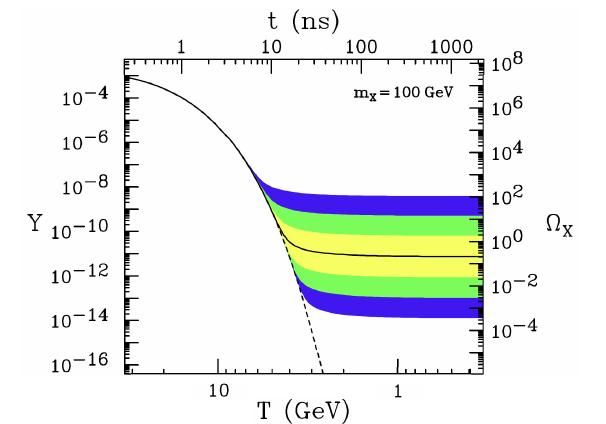
\includegraphics[width=0.75\textwidth]{DarkMatter/Freezeout}
%\caption{Evolution of WIMP number density (Y) and resulting thermal relic density (right) as a function of temperature T (bottom) and timet (top). The solid contour is for an annihilation cross section that yields the correct relic density, and the shaded regions are for cross sections that differr by 10, \SI{e2} and \SI{e3} from this value. The dashed contour is the number density of a particle that remains in thermal equilibrium. This image is taken from \cite{feng:DM}.}
%\label{fig:Freezeout}
%\end{figure}

Since WIMP DM candidates are particularly well-motivated, a robust experimental effort is underway to either discover DM, or constrain candidate theories. There are three main ways to detect DM which consist in the direct, indirect detection and production at colliders depending on wether the search is for DM candidates themselves or their annihilation products,

The direct detection consists in the search of WIMPs scattering from nuclei of ordinary matter. Since the nuclear recoil is very small, tipycally \SI{\sim 100}{\kev}, detectors capable of low energy detection thresholds, generally located underground, heve to be built. The indirect detection consists in the search of the products of the annihilation processes that occuring in the DM relic density.

All the kind of detection methods are gathered in a Feynman like diagram in \Fig{\ref{fig:detection}}.

\section{Detection strategies}
\begin{figure}[pt]
\centering
{\fontfamily{pag}\selectfont  
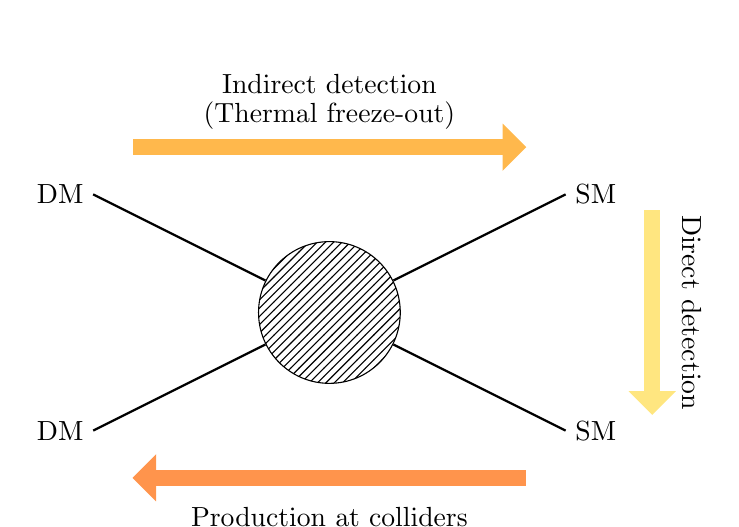
\begin{tikzpicture}
	\draw[thick] (-3,1.5) -- (3,-1.5);
	\draw[thick] (-3,-1.5) -- (3,1.5);
	\filldraw[white] (0,0) circle (0.9cm) ;
	\filldraw[pattern=north east lines] (0,0) circle (0.9cm) ;
	
	\node[left] at (-3,1.5){DM};
	\node[left] at (-3,-1.5){DM};
	\node[right] at (3,1.5){SM};
	\node[right] at (3,-1.5){SM};
	
	\draw[draw=none, fill=orange!80!yellow!70] (-2.5,2)--(2.3,2) -- (2.3,2.2) -- (-2.5,2.2);
	\draw[draw=none, fill=orange!80!yellow!70] (2.2,1.8) -- (2.5,2.1) -- (2.2,2.4) --cycle;
	\node[] at (0,2.9){Indirect detection};
	\node[] at (0,2.5){(Thermal freeze-out)};
	
	\draw[draw=none, fill=yellow!80!red!50] (4,1.3)--(4,-1.1) -- (4.2,-1.1) -- (4.2,1.3);
	\draw[draw=none, fill=yellow!80!red!50] (3.8,-1) -- (4.1,-1.3) -- (4.4,-1) --cycle;
	\node[rotate=-90] at (4.6,0){Direct detection};
	
	\draw[draw=none, fill=orange!80!red!70] (-2.3,-2)--(2.5,-2) -- (2.5,-2.2) -- (-2.3,-2.2);
	\draw[draw=none, fill=orange!80!red!70] (-2.2,-1.8) -- (-2.5,-2.1) -- (-2.2,-2.4) --cycle;
	\node[] at (0,-2.6){Production at colliders};
	
\end{tikzpicture}
}
\caption{Feynman like diagram che ho fatto io which illustrates different methods for dark matter particle detection. The direction of the time axis selects a particular process. In indirect detection Standard Model (SM) particles coming from Dark Matter (DM) decays are revealed.  In direct detction the recoil of nuclei from DM scattering is measured. At colliders SM particles collide to produce a pair of DM candidate.}
\label{fig:detection}
\end{figure}
\subsection{Direct Detection*}
The basic idea of Direct Detection is that if our galaxy is populated by WIMPs, a flux of them would run over our detectors and being detected. The WIMPs flux on the Earth is estimated to be of the order of \SI{e5}{\per \cm\squared\per\s}. The basic methodology for direct detection experiments is to look for this rare events that might be the signature of WIMP interactions, namely the elastic scattering of a WIMP on a target nucleus~\cite{snowmass}.

This kind of experiments must be carried out underground to reduce the signal contamination from every source of background. These sources come from cosmic rays, environmental radioactivity or detector radioactivity. For instance, two major experiments ongoing take place at LNGS, Italy, with the DAMA detector and followed by LIBRA, and in Modane, France, with the Edelweiss-III experiment at the LSM.
\begin{figure}[t]
\centering
\includegraphics[width=0.75\textwidth]{DarkMatter/damalibra}
\caption{Model-independent residual~\cite{damalibra} rate of the single-hit scintillation events, measured by the DAMA/LIBRA experiment in the \SIrange{2}{5}{\kev} energy intervals as a function of the time. The former DAMA experiment results are also shown. The zero of the time scale is January $1^{\text{st}}$ of the first year of data taking of the DAMA experiment. The superimposed curves represent the interpolated cosinusoidal function $A\cos{(t-t_0)}$. The dashed vertical lines indicate the maximum of the signal yield which occurs on June $2^{\text{nd}}$.}

\label{fig:damalibra}
\end{figure}

DAMA/LIBRA~\cite{damalibra} detector is made of 25 highly radiopure \ce{NaI}, doped with Tallium, crystal scintillators assembled in a $5\times5$ matrix, whose main strategy is to measure WIMPs flux by looking at its eventual periodic variation. The periodic change in WIMPs relative velocity wrt Earth orbiting around the Sun would lead to an annual modulation of the signal. Model independent results
%\footnote{i.e. measured rate of the single-hit events after subtracting the constant part $\avg{r_{ijk}-\text{flat}_{jk}}_{jk}$, where $r_{ijk}$ is the rate in the $i$-th time interval considered, for the $j$-th detector in the $k$-th energy bin and $\text{flat}_{jk}$ is the rate of the $j$-th detector in the $k$-th energy bin averaged over the annual cycles.}
, shown in \Fig{\ref{fig:damalibra}} for the interval \SIrange{2}{5}{\kev} in detected energy, actually show a modulation given by $A\cos{(t-t_0)}$ with period $T\simeq \SI{1}{year}$, a phase $t_0=\SI{152.2}{days}$ and an amplitude modulation $A =\SI{0.0204\pm0.0026}{counts/\kg/\keV}$. However DAMA/LIBRA results, providing a region in which WIMP can be found shown in \Fig{\ref{fig:WIMPcs}}, are a bit controversial. Indeed, they are not confirmed by other experiments such the mentioned Edelweiss-III.

Interactions between WIMPs and nucleon can be spin-dependent when the sign of the scattering amplitude depends on the relative orientation of particle spins, or spin-independent when spin orientations do not affect the amplitude. For spin dependent interactions, the WIMP effectively couples to the net nuclear spin, due to cancellation between opposite spin pairs. It will differ whether the net nuclear spin is carried by a residual neutron or proton, see \Fig{\ref{fig:WIMPcsSD}}. The spin-independent interaction is expected to be coherent within the entire nucleus, so that if a WIMP has equal coupling to protons and neutrons, the rate scales with the square of the atomic mass of the target nucleus. 

Actual experiments only put upper-limits on WIMPs mass, which are summarized in \Fig{\ref{fig:WIMPcs}} for several experiments making any hypotheses on their nature.

\begin{figure}[p]
\centering
\subfloat[][Spin-Dependent WIMP-proton cross sections]
{\includegraphics[width=0.45\textwidth]{DarkMatter/spindepProtons}}\quad
\subfloat[][Spin-Dependent WIMP-neutrons cross sections]
{\includegraphics[width=0.45\textwidth]{DarkMatter/spindepNeutrons}}

\caption{Constraints on spin-Dependent WIMP-proton cross sections WIMP-neutron cross sections  as a function of WIMP
mass as of Summer 2013}
\label{fig:WIMPcsSD}
\end{figure}

\begin{figure}[p]
\centering
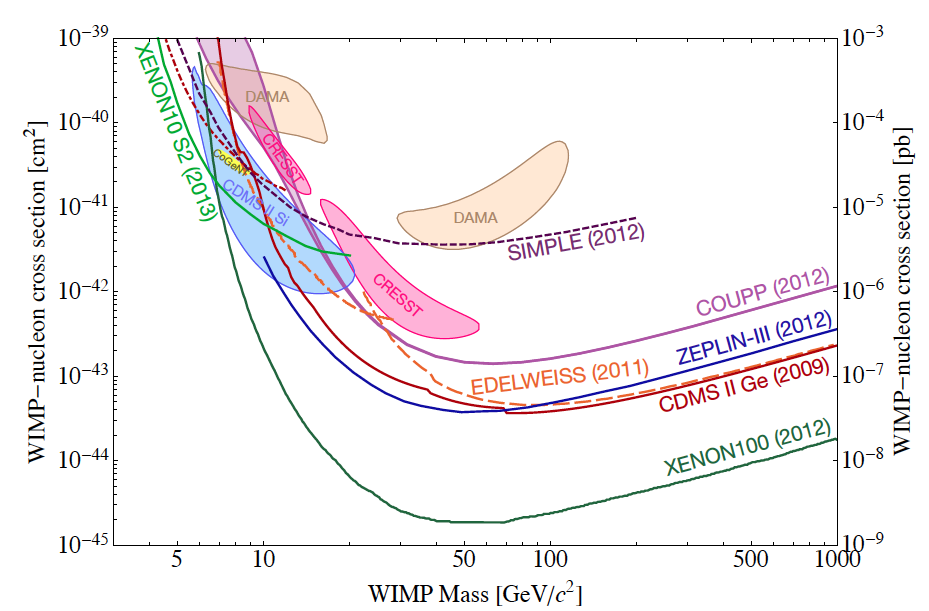
\includegraphics[width=0.75\textwidth]{DarkMatter/WIMPcs}
\caption{Constraints on spin-independent WIMP-nucleon cross section vs WIMP mass as of summer 2013.}
\label{fig:WIMPcs}
\end{figure}

\subsection{Indirect Detection}
The idea of Indirect Detection is to search for the products of the DM annihilation processes  happening in regions of the Universe where DM density is supposed to be higher like the center of the galaxy. Annihilation probability increases with DM density in a certain region of space and it produces SM particles such gamma rays, neutrinos, positrons, antiprotons. Therefore WIMPs can be detected by detecting these particles.

The disadvantage associated with Indirect Detection is the background induced by ``ordinary'' astrophysics. If considering only the signal strength from DM annihilations, the best target to detect anihilation products would be the galactic center, but there is a relatively unconstrained astrophysical background to any signals that could be produced there. Many research in the galactic center found signals consistent with DM annihilation but also compatible with the background and statistical fluctuations.

\subsection{Production at colliders}
The production at colliders share the same idea of direct detection: if a WIMP can scatter from a nucleon, it can be produced in \pp collision at high energy from scattering against SM particles. Common to all collider DM searches is the signature of missing transverse momentum (\met) caused by the WIMPs escaping the detector. Therefore a striking proof of Dark Matter candidates production may be verified from an inbalance in the visible transverse momentum in the event.

Nevertheless we cannot tag \met as the only final state of a collision. Indeed, the experimental signature consists in a large value of \met and a back-to-back topology between \met and the Standard Model particle used for tagging the event, i.e in order to detect a possible WIMP, it must be associated with a detectable object. This kind of analises are called \emph{Mono-X}. They are characterized by large missing transverse momentum and an energetic particle (the \emph{X}) such a jet (Mono-jet), a photon (\mph) or a \Wboson or \Zboson boson.

DM collider searches can be achieved in different ways. The first is to probe specific theories and models, and checking every decay channel predicted by a specific theory. This happens in every SUSY research for which every analysis is higly optimized for particular model. Another way is to reveal DM particles as the only accessible new state to an experiment.

%Once produced, DM will pass through the detector without leaving any tracks and without decaying into other particlese, as if it were a neutrino, since the iwe assumed that DM is weakly interacting and stable enough.

At the LHC, the MonoJet is the most sensitive search. On the other hand the \mph analysis, even if it works better at lepton colliders, at LHC prvovides good sensitivity and a very clean signature is achieved due to the request of a photon.

\section{The Minimal Dark Matter model}
The Minimal Dark Matter (DM) model~\cite{Cirelli:paper} extends the SM with a Electroweak (EW) fermion triplet,as a minimal candidate for WIMP DM. This candidate ($\chi$) is triplet under $SU(2)_L$, where the subscript L indicates coupling only to left-handed fermions, and singlet under color and hypercharge ($Y=0$). Its relevant Lagrangian is very simple and reads:
\begin{equation}
\begin{split}
\mathcal{L}_\chi&=\frac{1}{2}\bar{\chi}\left(i\slashed{D}-M_\chi\right)\chi \\
			&= \frac{1}{2}\bar{\chi_0}\left(i\slashed{\partial}-M_{\chi_0}\right)\chi_0+\bar{\chi}^+\left(i\slashed{\partial}-M_{\chi^\pm}\right)\chi^+ \\
			&+ g \left(\bar{\chi}^+\gamma_\mu\chi^+\left(s_w A_\mu + c_w Z_\mu \right) +\bar{\chi}^+ \gamma_\mu\chi_0W^-_\mu + \bar{\chi_0}\gamma_\mu\chi^+W^+_\mu \right)
\end{split}
\end{equation}
where $g$ is the $SU(2)$ gauge coupling, and $s_w$ and $c_w$ are the sine and the cosine of the Weinberg angle.

All the possible interactions between $\chi$ and other SM particles are required to preserve the gauge and the symmetries of the SM particularly the lepton number under which $\chi$ is assumed to be neutral. This last requirement is crucial, since it forbids the presence of higher dimensional operator that could lead a decay of $\chi$.  The difference at two loop level of $M_{\chi^\pm} - M_{\chi_0}$ is  about \SIrange{164}{165}{\mev}. This constrain was not applied to an eventual 5-plet particle which would have been automatically stable anyway. On the other hand the triplet has important features even beyond the DM motivation~\cite{Cirelli:paper} and it is capable to be produced at collider rather \mbox{than the 5-plet}.

If one requires that $\chi$ is thermally produced via the freeze-out mechanism discussed in \Sect{\ref{sec:wimp}}, and that it constitues all the DM in the Universe, then we can extimate its mass to be \SIrange{3.0}{3.2}{\tev}. This range of mass, of course, is out of reach from LHC. Nevertheless for masses lower than \SI{3}{\tev}, $\chi$ is a subdominant DM component if thermally produced and its existence is again well justified to pursue any search at colliders. So the Minimal DM model can be seen as a benchmark of the typical thermal-relic WIMP Dark Matter candidate, being a prototype for more complicated models, reproducing their low energy phenomenology with great accuracy.

As mentioned in the previous section, a way to search for WIMPs at colliders is via the so-called \emph{Mono-X} analyses. In this kind of searches the signal comes not only for the $\chi_0$ WIMP candidate particle but also from its two charged partners in the triplet. We can assume that the latter decay via a $\chi_0$ and soft, or low-momentum, charged pions (\pipm) both unreconstructed in the detector. 

A different, possible, scenario is that the tail of the decay distribution of the two charged $\chi$s might also leave tracks in the detector. These tracks would end when they decay as described into a couple of $\chi_0$ and charged pions. For that reason the \emph{disappearing tracks} would provide the most sensitive probe to the Minimal Model, but also the most challenging from the experimental view perspective.

\smallskip
In this work a \mph analisys has been pursued following the lead of the one carried on in 2017 by the ATLAS Collaboration~\cite{paperMP}. In this context the \mph results were re-interpreted in terms of the Minimal Dark Matter model.











\clearpage
\thispagestyle{empty}
\chapter[MonteCarlo samples production]{MonteCarlo production of Minimal DM model samples for the \mph analysis}

\lettrine{T}{}his chapter describes all the steps made to generate, simulate and reconstruct MonteCarlo (MC) events in the context of the Minimal DM model for the \mph analysis .

%In the \mph analysis, which is a ``cut\&count'' analysis (refer to Chapt. \ref{chapt:mph}), we are looking for a single high energy photon and large missing transverse momentum (\met) signature, whose definition will be given in \Sect{\ref{sec:recoreal}}. Therefore it is characterized by a relative clean final state thanks also to a small set of SM processes that produces the same outcome. The Minimal DM model predicts several ways in which DM can be produced and revealed within a \mph analysis. Three examples of Feynman diagram are given in \Fig{\ref{fig:feynman}}. Notice that a photon can also be radiated from the final state which is a peculiarity with respect to other DM simplified models adopted at LHC.

The simulation of the physics processes in the detector is a fundamental ingredient in the analysis to assess the discovery potential for a new signal but also as input to the real data scrutiny.
%In order to study the detector response for a wide range of physics processes and scenarios, 
A detailed simulation  of the physics process and of the detector response is pursued providing an output format which is identical to that of the true detector. 

The simulation process of events comes across several steps. The first one is the event generation in which the products of \pp collision are simulated. The event generation starts with the creation of the list of particles (electrons, photons, partons\dots) from the hard scattering. The partons radiation is modeled through \emph{parton shower}, finally hadronization and underlying events are also used to complete the event. This step consists in the Truth-level simulation, producing an EVNT file, and a summary file (a TRUTH file) can be built from this events at particle level.

The second step consists in the simulation of how particles interact with the detector which is followed by the digitization step. The simulation program is integrated into the ATLAS software framework, Athena, and uses the \geant \cite{geant4} simulation toolkit. Detailed description of the ATLAS Simulation Infrastructure is given in~\cite{simulation}.

Afterwards the simulated event can be passed to the reconstruction software in the same way as actual recorded data. Then all the events reconstructed are filtered by a derivation code which selects only the  relevant events for a specific analysis. Finally the ``derivated'' events are collected in a compact and practical RooT file, i.e a \emph{NTUPLE}, ready to be processed by the analysis.

For this analysis the software chain described above, and shown in \Fig{\ref{fig:chain}}, was run in batch mode on the Milano Tier3 computing facility via HTCondor$^{\textup{TM}}$.


\begin{figure}[t]
\centering
{\fontfamily{pag}\selectfont  
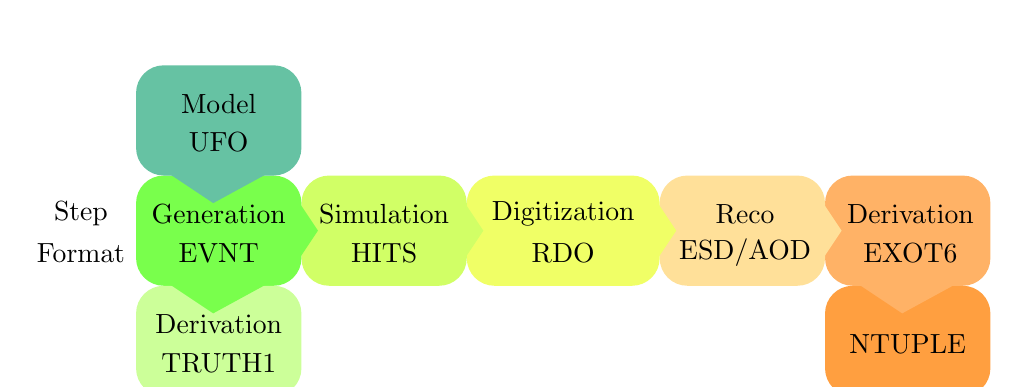
\begin{tikzpicture}[scale=0.7]

	\node[] at (-1,1.3){Step};
 	\node[] at (-1,0.6){Format};
 	
 	\draw[draw=none,fill=orange!75!, rounded corners=10pt] (12.5,0) rectangle +(3,-2);
 	\node[] at (1.5+12.5,-2+0.6+.35){NTUPLE};
 	
	\draw[draw=none,fill=orange!60!, rounded corners=10pt] (12.5,0) rectangle +(3,2);
 	\draw[draw=none,fill=orange!60!] (13,0.1)--(1.4+12.5,-0.5)--(2.5+12.5,0.1) -- cycle;
 	\node[] at (7.75+6.3,1.3){Derivation};
 	\node[] at (7.75+6.3,0.6){EXOT6};
	
	\draw[draw=none,fill=yellow!40!orange!40,rounded corners=10pt] (9.5,0) rectangle +(3,2);
 	\draw[draw=none,fill=yellow!40!orange!40] (12.4,0.4)--(12.8,1)--(12.4,1.6) -- cycle;
 	\node[] at (7.75+3.3,1.3){Reco};
 	\node[] at (7.75+3.3,0.6){ESD/AOD};
	
	\draw[draw=none,fill=green!10!yellow!60,rounded corners=10pt] (6,0) rectangle +(3.5,2);
 	\draw[draw=none,fill=green!10!yellow!60] (9.4,0.4)--(9.8,1)--(9.4,1.6) -- cycle;
 	\node[] at (7.75,1.3){Digitization};
 	\node[] at (7.75,0.6){RDO};
	
	\draw[draw=none,fill=green!30!yellow!60,rounded corners=10pt] (3,0) rectangle +(3,2);
 	\draw[draw=none,fill=green!30!yellow!60] (5.9,0.4)--(6.3,1)--(5.9,1.6) -- cycle;
 	\node[] at (4.5,1.3){Simulation};
 	\node[] at (4.5,0.6){HITS};
 	
 	\draw[draw=none,fill=green!75!yellow!70,rounded corners=10pt] (0,0) rectangle +(3,2);
	\draw[draw=none,fill=green!50!yellow!40,rounded corners=10pt] (0,0) rectangle +(3,-2);
 	\draw[draw=none,fill=green!75!yellow!70] (2.9,0.4)--(3.3,1)--(2.9,1.6) -- cycle;
 	\draw[draw=none,fill=green!75!yellow!70] (.5,0.1)--(1.4,-0.5)--(2.5,0.1) -- cycle;
 	
 	\node[] at (1.5,1.3){Generation};
 	\node[] at (1.5,0.6){EVNT};
 	\node[] at (1.5,-2+1.3){Derivation};
 	\node[] at (1.5,-2+0.6){TRUTH1};
 	
 	\draw[draw=none,fill=green!60!blue!60,rounded corners=10pt] (0,2) rectangle +(3,2);
 	\draw[draw=none,fill=green!60!blue!60] (.5,2.1)--(1.4,1.5)--(2.5,2.1) -- cycle;
 	\node[] at (1.5,3.3){Model};
 	\node[] at (1.5,2.6){UFO};
 	
 	%\node[] at (10.5,1.3){Reconstruction};
 	%\node[] at (10.5,0.6){ESD/AOD};

	%\node[ single arrow , draw, single arrow head extend=.7cm, gray!50, black] at (3.3,0.8) {    };
\end{tikzpicture}
}
\caption{The ATLAS simulation chain. The theoretical model is implemented in a UFO file and given as input to the generation program. Truth level analysis can be pursued, or the EVNT file can be used in a detector simulation whose outcome will be digitized in a RawData Object file and reconstructed in Event Summary Data (ESD) and Analysis Object Data (AOD). A derivation framework runs over the AOD to get the relevant events for a specific analysis. The Derivated Analysis Object Data (DAOD), which in our case is an EXOT6 file, can be made readable by RooT in a NTUPLE form.}
\label{fig:chain}
\end{figure}


\section{Generation}
 \begin{figure}[tp]
 \centering
 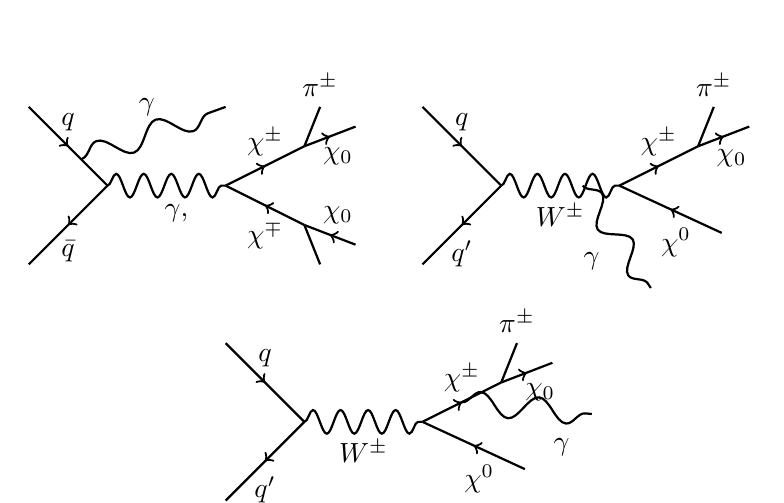
\begin{tikzpicture}
 [scale=0.5,decoration={
markings,% switch on markings
mark=% actually add a mark
at position .5  with {\arrow{>}}}]
 \draw[thick, postaction={decorate}] (-4,2) node at(-3,1)[above=2pt] {  $q$} -- (-2,0) ;
 \draw[thick, postaction={decorate}] (-2,0) -- (-4,-2) node at(-3,-1) [below=2pt] {  $\bar{q}$} ;
 \draw[thick,decorate,decoration={snake,amplitude=1.5mm,segment length=3.5mm}] (-2,0)--(1,0) node  at (-0.25,0) [below=3pt]{  $\gamma$,$\Zboson$};
 \draw[thick, postaction={decorate}] (1,0) -- (3,1) node at (2,0.5) [above]  {  $\chi^{\pm}$} ;
 \draw[thick, postaction={decorate}] (3,-1) --(1,0) node at (2,-0.5) [below=2pt]  {  $\chi^{\mp}$} ;
\draw[thick](3,1)--(3.4,2) node[above] {  $\pi^{\pm}$};
\draw[thick,postaction={decorate}](3,1)--(4.3,1.5) node[right=5pt,below] at (3.5,1.24) {  $\chi_0$};
\draw[thick](3,-1)--(3.4,-2) node[below] {  $\pimp$};
\draw[thick,postaction={decorate}](4.3,-1.5)--(3,-1) node[right=5pt,above] at (3.5,-1.24) {  $\chi_0$};
\draw[thick,decorate,decoration={snake,amplitude=1.5mm,segment length=8mm}] (-2.65,0.68)--(1,2) node at (-1,1.5) [above]{  $\gamma$};


 \draw[thick, postaction={decorate}] (-4+10,2) node at(-3+10,1)[above=2pt] {  $q$} -- (-2+10,0) ;
 \draw[thick, postaction={decorate}] (-2+10,0) -- (-4+10,-2) node at(-3+10,-1) [below=2pt] {  ${q'}$} ;
 \draw[thick,decorate,decoration={snake,amplitude=1.5mm,segment length=3.5mm}] (-2+10,0)--(1+10,0) node  at (-0.5+10,0) [below=3pt]{  $W^{\pm}$};
 \draw[thick, postaction={decorate}] (1+10,0) -- (3+10,1) node at (2+10,0.5) [above]  {  $\chi^{\pm}$} ;
 \draw[thick, postaction={decorate}] (3.6+10,-1.2) --(1+10,0) node at (1.8+10,-0.6) [below=12pt, right]  {  $\chi^{0}$} ;
\draw[thick](3+10,1)--(3.4+10,2) node[above] {  $\pi^{\pm}$};
\draw[thick,postaction={decorate}](3+10,1)--(4.3+10,1.5) node[right=5pt,below=1pt] at (3.5+10,1.24) {  $\chi_0$};

\draw[thick,decorate,decoration={snake,amplitude=1.5mm,segment length=7mm}] (0.07+10,0)--(1.8+10,-2.6) node at (0.9+10,-1.3) [below left=2pt]{  $\gamma$};

 \draw[thick, postaction={decorate}] (-4+5,2-6) node at(-3+5,1-6)[above=2pt] {  $q$} -- (-2+5,0-6) ;
 \draw[thick, postaction={decorate}] (-2+5,0-6) -- (-4+5,-2-6) node at(-3+5,-1-6) [below=2pt] {  ${q'}$} ;
 \draw[thick,decorate,decoration={snake,amplitude=1.5mm,segment length=3.5mm}] (-2+5,0-6)--(1+5,0-6) node  at (-0.5+5,0-6) [below=3pt]{  $W^{\pm}$};
 \draw[thick, postaction={decorate}] (1+5,0-6) -- (3+5,1-6) node at (2+5,0.5-6) [above]  {  $\chi^{\pm}$} ;
 \draw[thick, postaction={decorate}] (3.6+5,-1.2-6) --(1+5,0-6) node at (1.8+5,-0.6-6) [below=12pt, right]  {  $\chi^{0}$} ;
\draw[thick](3+5,1-6)--(3.4+5,2-6) node[above] {  $\pi^{\pm}$};
\draw[thick,postaction={decorate}](3+5,1-6)--(4.3+5,1.5-6) node[right=7pt,below] at (3.5+5,1.24-6) {  $\chi_0$};

\draw[thick,decorate,decoration={snake,amplitude=1.5mm,segment length=7.4mm}] (2+5,0.5-6)--(5.3+5,0.2-6) node at (3.65+5,0.35-6) [below=14pt,right=6pt]{ $\gamma$};
\end{tikzpicture}
\caption{Illustration of some Feynman diagrams for \mph processes in the Minimal DM Model.}
\label{fig:feynman}
\end{figure}
For the event generation process \MGMCatNLO v2.4.0 was used~\cite{madgraph}. This software automatically generates matrix elements, as for example decays or scattering from a couple of particles. The user simply specifies the process of interest by giving the initial and final state particles and \MADGRAPH generates the Feynman diagrams and the code needed for the calculation of the matrix elements~\cite{Pottgen:2016807}. In this context, even if the software could generate matrix element up to the next to leading order (\NLO) only leading order (\LO) calculations were used.

The Minimal DM Model was already been implemented in an UFO file containing its details~\cite{mperego} considering the pure electroweak triplet (\chip\!, \chizero\!, \chim\!) and implemented in FeynRules. UFO is the format used in input by \MADGRAPH. Although the model would predict a mass splitting of \SI{\sim 165}{\mev} between \chipm and the \chizero, here is set to be \SI{1}{\gev}: small enough to let the charged $\chi$s decay into soft pions and a \chizero but large enough not to create issues in the generation program. 

Events of the type: 
\begin{gather*}
p p \rarrow \chi^+ \chi^- \gamma,\, \chi^+ \rarrow \piplus \chi_0,\, \chi^- \rarrow \piminus \chi_0\\
p p \rarrow \chi^+ \chi_0 \gamma,\, \chi^+ \rarrow \piplus \chi_0\\
p p \rarrow \chi^+ \chi_0 \gamma,\, \chi^- \rarrow \piminus \chi_0
\end{gather*}
have been generated to provide a final stare characterized by one photon and missing transverse momentum (\met). The Minimal DM model predicts several ways in which DM can be produced and revealed within a \mph analysis. Three examples of Feynman diagram are given in \Fig{\ref{fig:feynman}}. Notice that a photon can also be radiated from the final state which is a peculiarity with respect to other DM simplified models adopted at LHC.

For 21 different $\chi_0$ masses, \num{10000} events have been generated requiring a kinematic cut on photon energy to be greater than \SI{130}{\gev} in order to populate the \mph analysis phase space.

Before performing the hadronization and parton shower, a fast scan for different mass point running \MADGRAPH \emph{on-the-fly} was made in order to get an order the values of the cross sections. Results are reported in \Tab{\ref{tab:xsectheo}}.

\begin{table}[pt]
\centering
\begin{tabular}{ccc}
\toprule
Mass[GeV]&Cross section [pb]&Error [pb]\\
\midrule
\num{1}& \num{0.3069}& \num{0.0020}\\
\num{10}& \num{0.2924}& \num{0.0020}\\
\num{50}& \num{0.01571}& \num{0.00013}\\
\num{100}& \num{4.67e-03 }& \num{0.03e-03}\\
\num{200}& \num{1.164e-03}& \num{0.009e-03}\\
\num{500}& \num{7.54e-05}&\num{0.05e-05}\\
\num{750}& \num{1.369e-05}& \num{0.009e-05}\\
\num{1000}& \num{3.169e-06}& \num{0.021e-06}\\
\bottomrule
\end{tabular}
\caption{Table listing the cross section expected from theory, for several mass points.}
\label{tab:xsectheo}
\end{table}

For the simulation of the parton showers, underlying event and hadronization, the output of \MADGRAPH has to be passed to an external programm, which in our case is \PYTHIA v8.210~\cite{pythia}. This framework accounts for the generation, starting from a \emph{Les Houches Event} (LHE) file, of parton shower and underlying event, i.e. it creates colourless states from free quarks and gluons. \PYTHIA was set up with NNPDF23LO PDF and the A14 tuning. The output file produced is an EVNT file which can be used as input either for the detector simulation step or to produce a TRUTH file.

\subsection{Truth level validation}
\label{sec:truth}
The generation of the events as it were ``in vacuum'' is called \emph{Truth level}. Here no assumptions are made on the detector, but we only want to analyze the process and its outcome. The TRUTH1 is a file format coming from a Derivation framework, which will be better explained in \Sect{\ref{sec:derivation}}, and it contains all needed information at particle level.

A ``fiducial region'' can be defined t allow the re-interpretation of the data analysis results in terms of new physiscs models, like the Minimal DM model, providing useful contraints.
 
The pre-selection for \mph analysis, (\Sect{\ref{sec:SRselection}}), involves:
\begin{itemize}
\item photons with $\pt^\gamma>\SI{10}{\GeV}$ with $\abs{\eta_\gamma}<2.37$ and $1.37<\abs{\eta_\gamma}<1.52$;
\item electrons with $\pt^e>\SI{7}{\gev}$ with $\abs{\eta_e}<2.47$;
\item muons with $\pt^\mu>\SI{6}{\gev}$ with $\abs{\eta_\mu}<2.5$;
\item jets with $\ptjet>\SI{30}{\gev}$ with $\abs{\eta_{\textup{jet}}}<4.5$ not overlapping with electron or photon by $\DeltaR > 0.4$;
\end{itemize}
while the actual selection requires:
\begin{itemize}
\item $\met>\SI{150}{\gev}$;
\item leading photon with $\pt^\gamma > \SI{150}{\GeV}$;
\item \met significance: $\met/\sqrt{\sumET} > \SI{8.5}{\GeV^{1/2}}$;
\item no electrons nor muons and $N_\textup{jets}\le 1$ with $\Delta\phi_\textup{jet-\met}<0.4$ if any.
\end{itemize}

The validation of the TRUTH files produced for several \chizero masses consists in the check of the distribution of the main kinematic variables involved in the analysis. The results are shown in validation plots in \Fig{\ref{fig:validation}} after the first four cuts provided above, for different DM masses. Notice that the peak for low-$\pt^\gamma$ in \Fig{\ref{subfig:phpt}} rises because the leading photon could enter the crack region (\etaRange{1.37}{1.52}) and therefore doesn't pass the $\eta$ cuts, then the code select a subleading photon with lower momentum
%\footnote{A weird behaviour has been noticed in \PYTHIA for which sometimes the leading photon converts in a couple $e^+e^-$ for apparently no reasons. These events, however, contribute to the sharp low peak but they occur in the 5\% of the case and they can be neglected}. 
Detailed analyisis on these events in terms of fiducial cross section will be given in \Sect{\ref{sec:fid}}.

\begin{figure}[t]
\centering
\subfloat[][Photon momentum for different masses. \label{subfig:phpt}]
{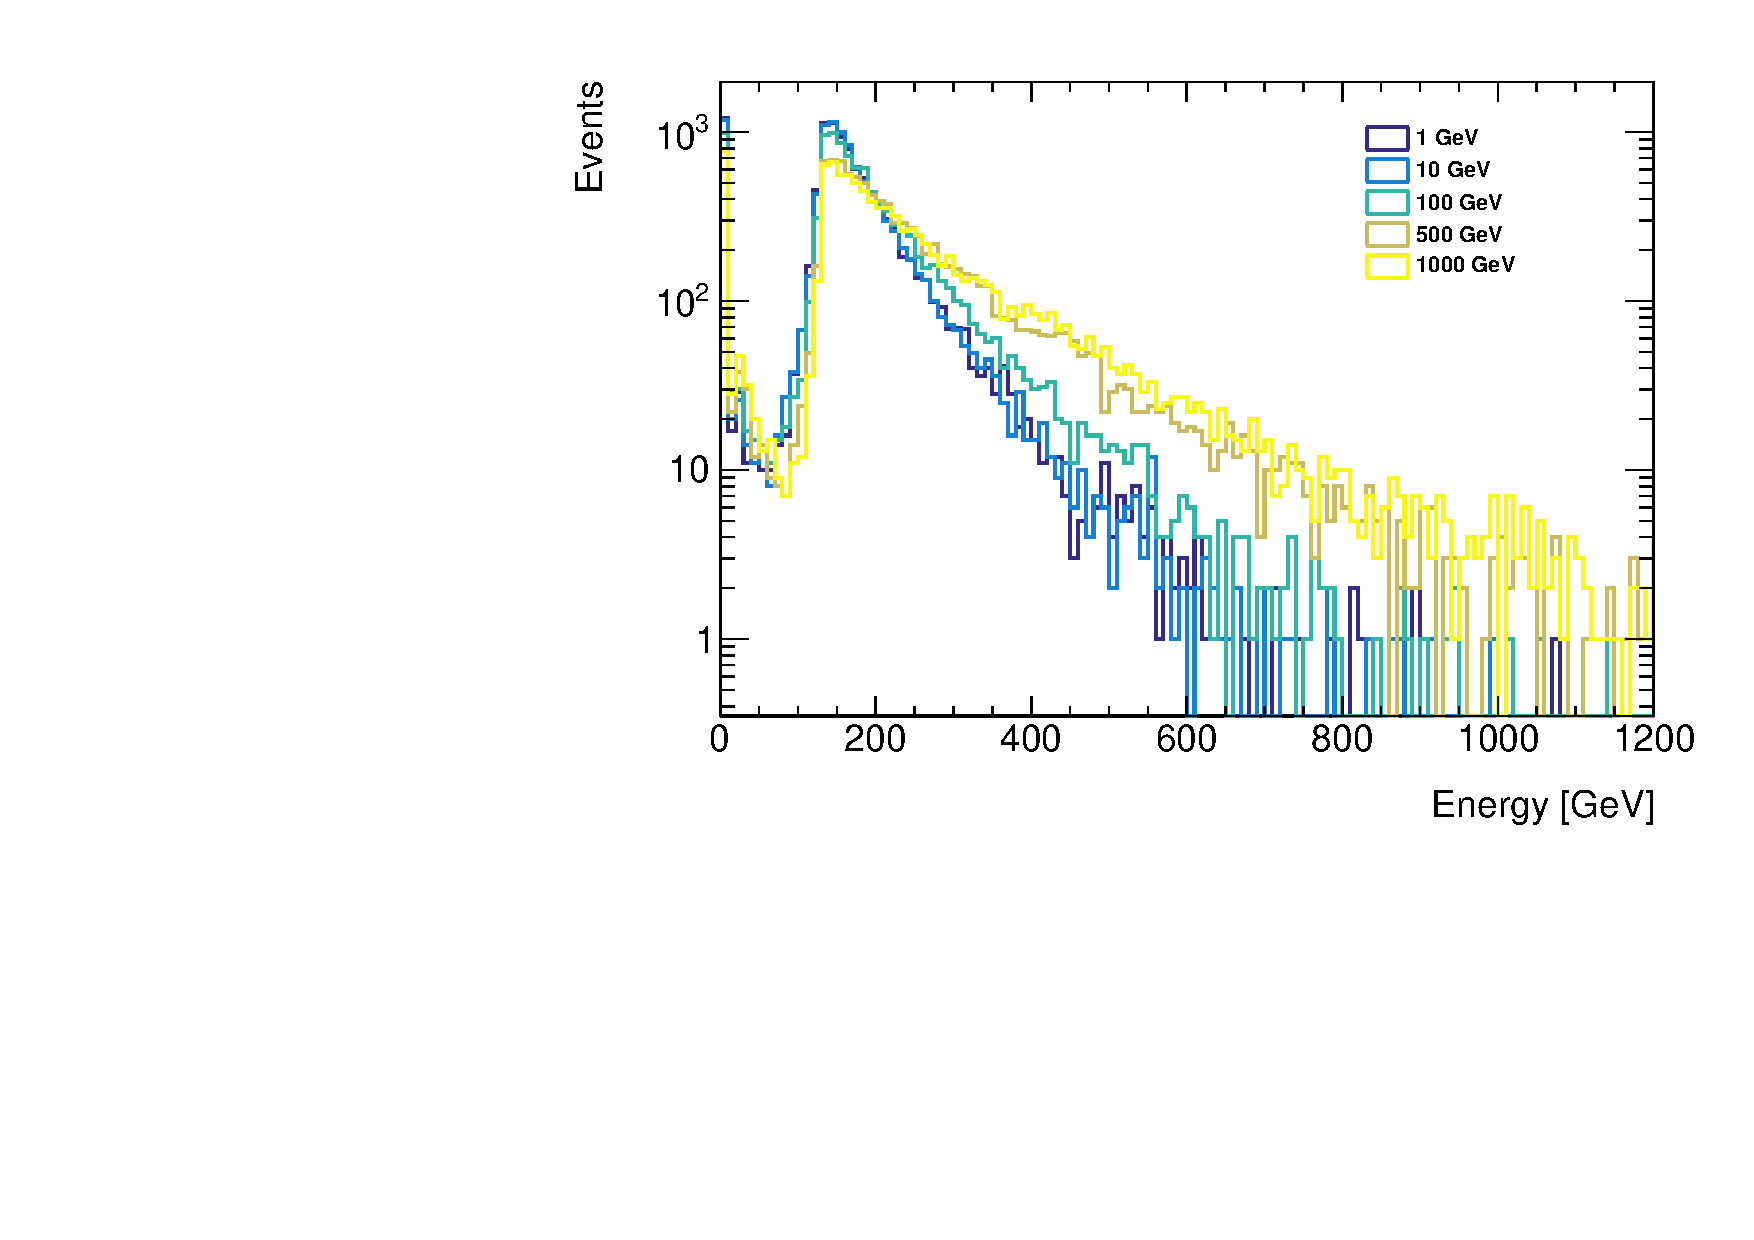
\includegraphics[width=.45\textwidth]{MCSample/canPhPtoverlap}} \quad
\subfloat[][Missing energy for different masses]
{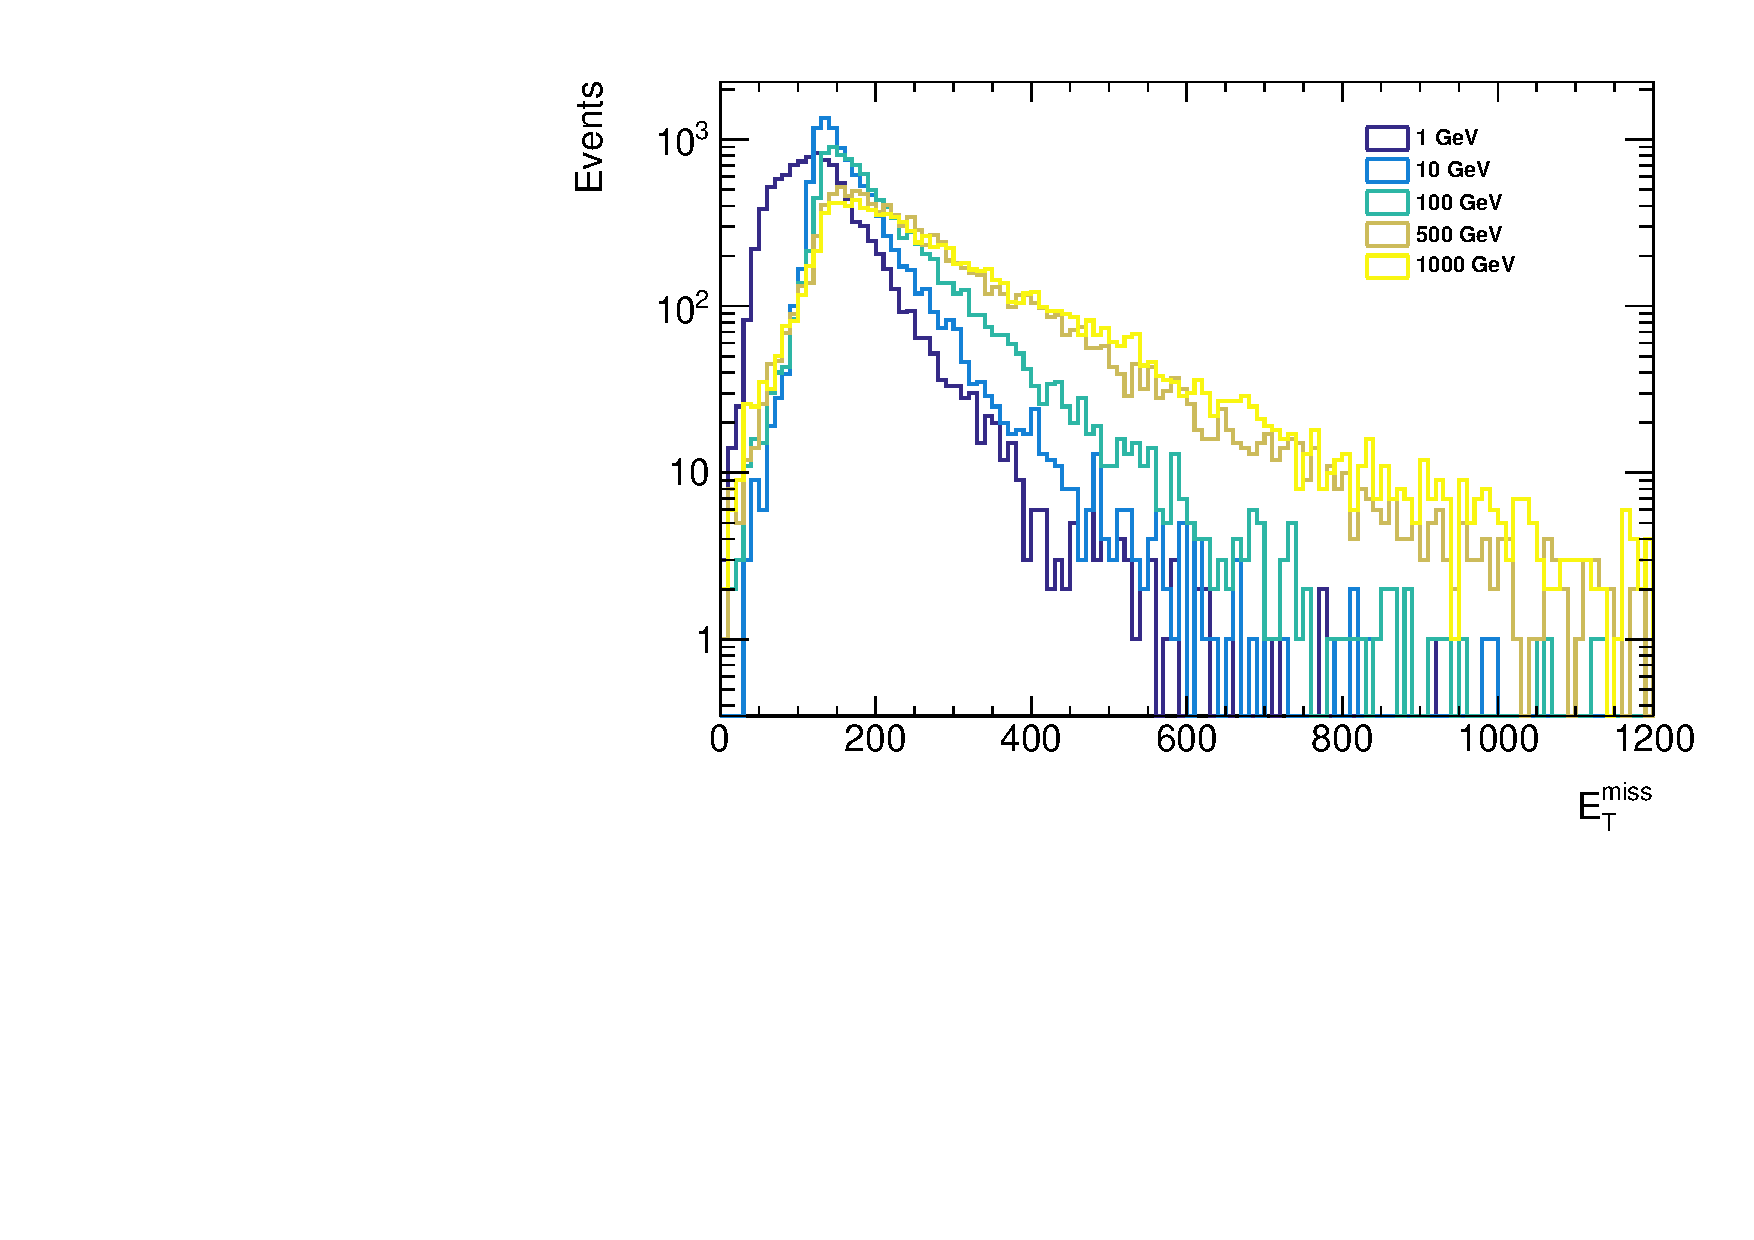
\includegraphics[width=.45\textwidth]{MCSample/canMEToverlap}} \quad
\subfloat[][Pseudorapidity of the photon for different masses]
{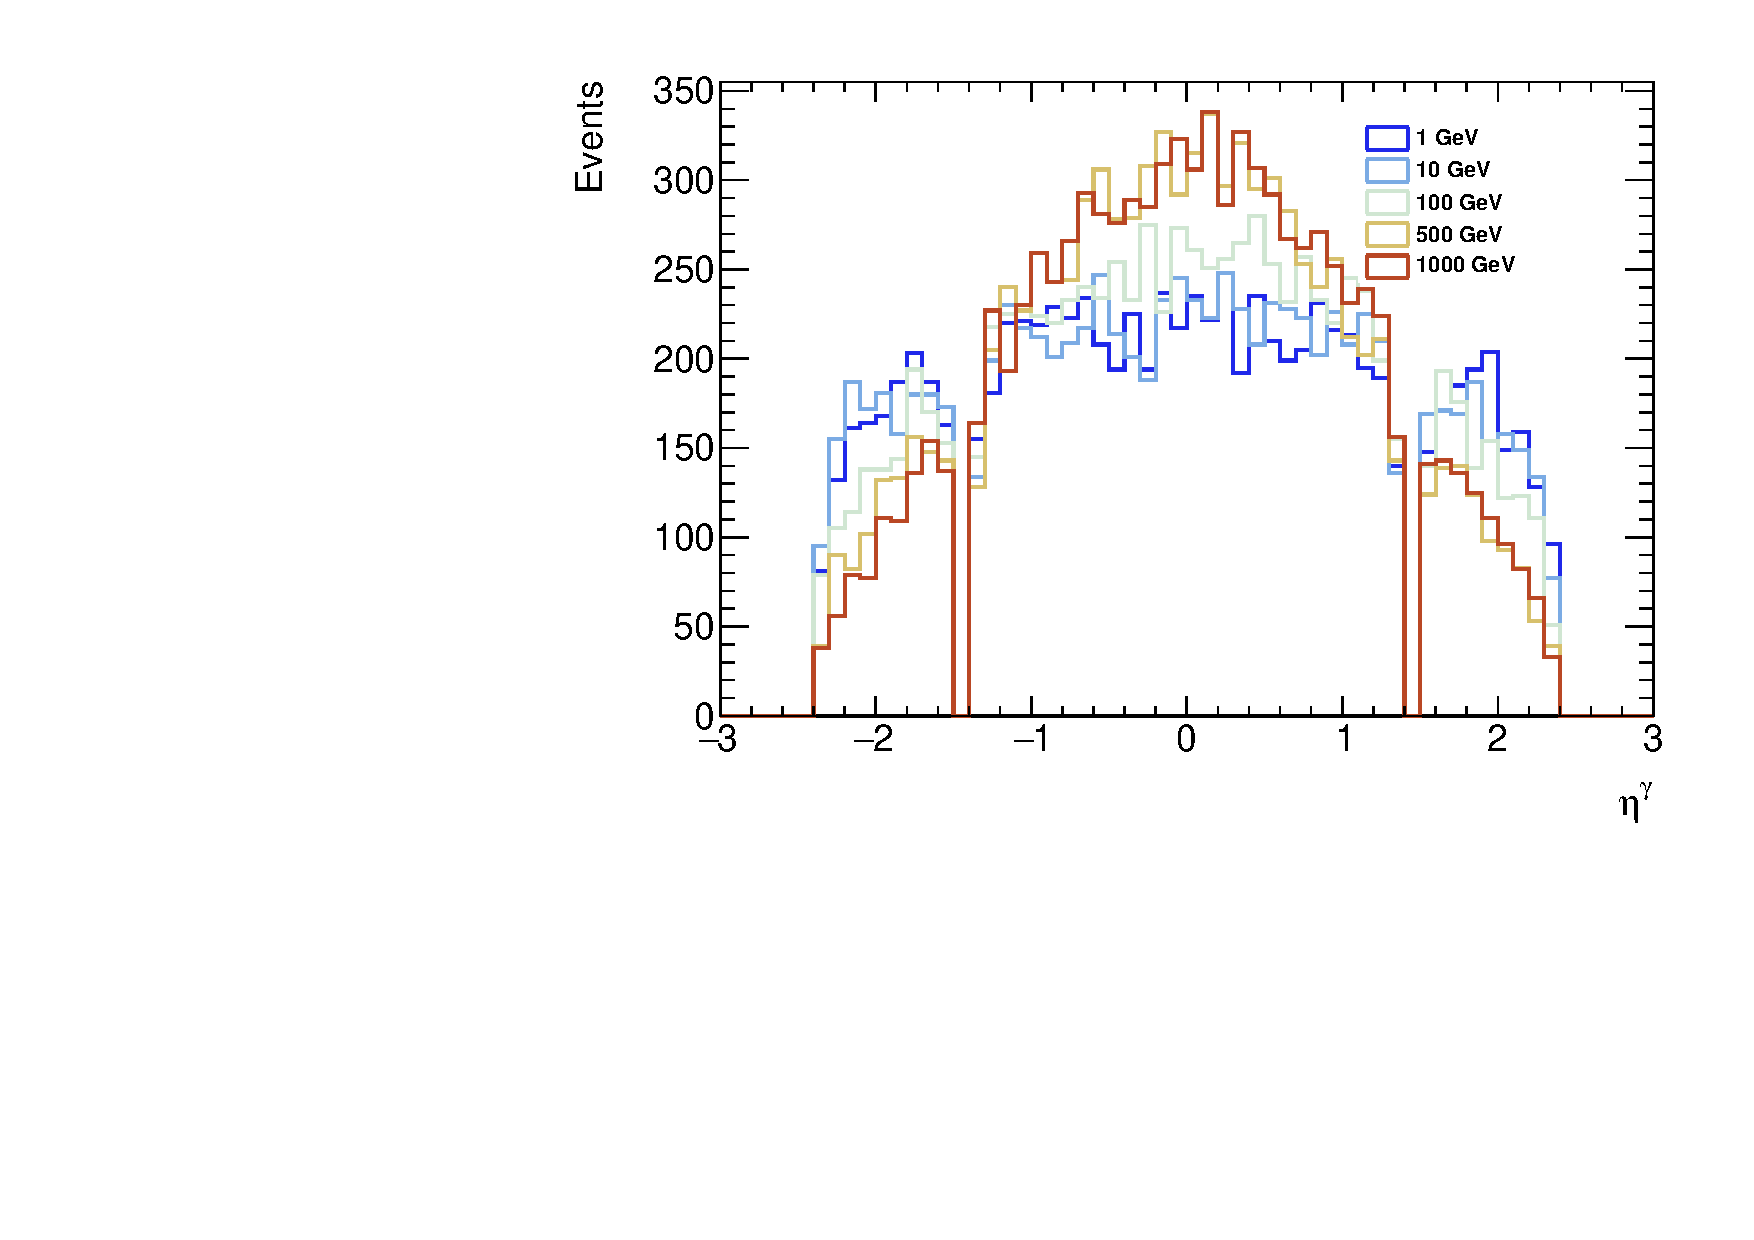
\includegraphics[width=.45\textwidth]{MCSample/canEtaoverlap}} \quad
\subfloat[][Number of jets for different masses]
{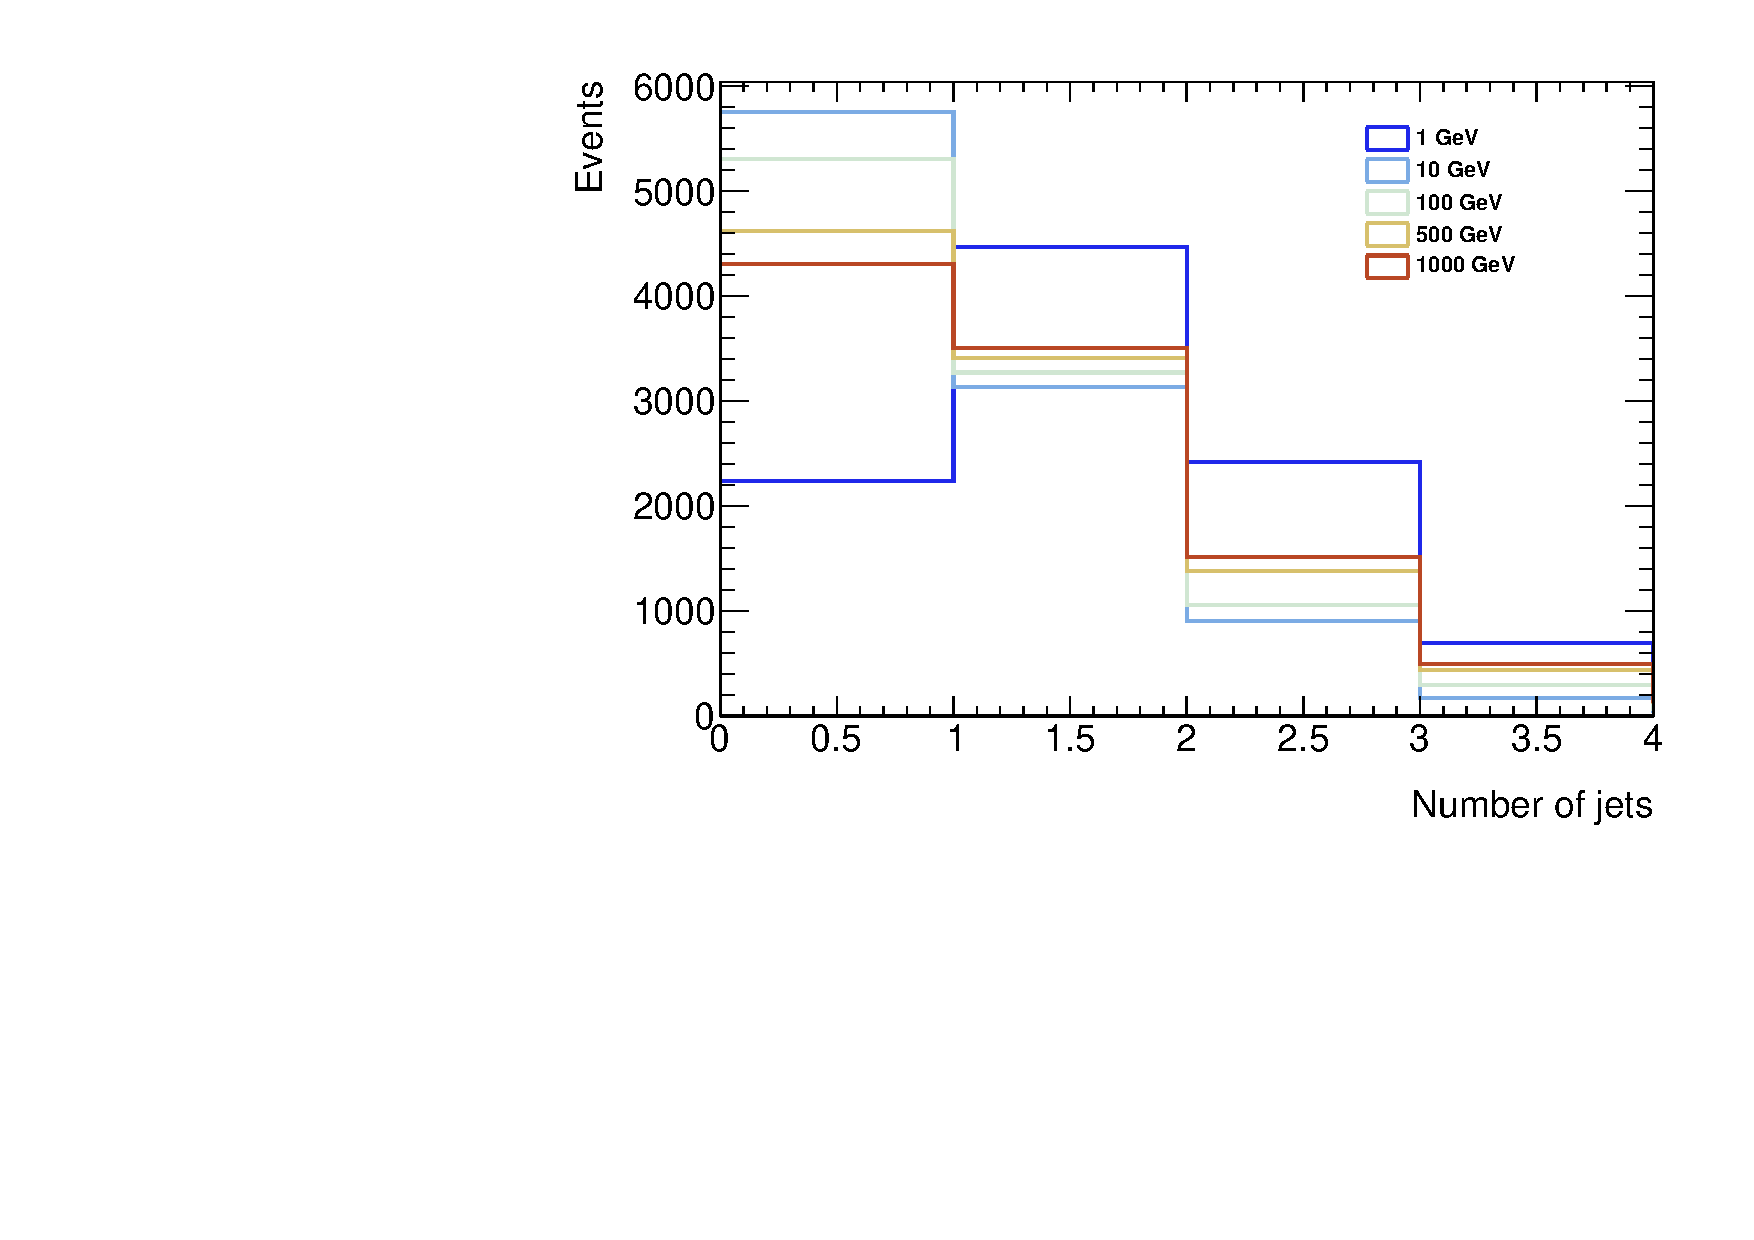
\includegraphics[width=.45\textwidth]{MCSample/canNjetsoverlap}} \quad
\caption{Validation plots for the Minimal DM model. From these plots the evolution of the main kinematics variables can be seen as a function of DM mass. These plots are generated after the pre-selection cuts given in \Sect{\ref{sec:truth}}}
\label{fig:validation}
\end{figure}

\section{Simulation}
The standard simulation of ATLAS relies on the \geant particle simulation toolkit to simulate the interaction of particles with matter. This step takes as inpunt the EVNT file from \PYTHIA, in our case, or any of the generators such \HERWIG and \SHERPA, and it is the most time expensive stage in the full simulation. The output is stored into an HIT file. To save time the framework allows the user to skip a certain number of events at the beginning of an input file by submitting $n$ jobs with $N$ events each to a $n\times N$ event input file and merged together at the end of the process.

%First of all comes the simulation initialization which is divided in three steps. Stage one of the initialization occurs as soon as Athena is started which is set to AtlasProduction 19.2.4.9. release. Here job properties provided by the user are locked, metadata that will be stored with the hit output file are gathered and the HIT file initialized. Finally service is created to interface with \geant which is not fully initialized at this stage. In stage two detector, physics regions, range cuts are created. Each piece of the ATLAS detector is constructed in GeoModel according to the geometry chosen, which in this work is \verb!ATLAS-R2-2015-03-01-00_VALIDATION!, and translated into an equivalent \geant geometry. Next, the Monte Carlo truth strategies, which are \verb!MC12! in this context, are added to the simulation.Then the magnetic field is loaded and every user action, which allows a user to insert pieces of code in various places throughout the simulation event loop, provided from the configuration command are initialized. The physics list (see below) used for simulation is also set at this point. The third stage completes the job preparation. assigning fast simulation models and runs \geant  software.

%A physics list contains all numerical models that describe the particles' interactions in the \geant simulation. The \geant Collaboration provides several combinations of these models for every possible physical outline. We used the \verb!FTFP_BERT! phisics list which is the current \geant default. Any further information can be found in~\cite{ftfpbert}.

To speed up the full simulation process a fast simulation approach is adopted. In this work ATLFAST-II was used, which provides large statistics to supplement full simulation studies. It is made up from two components: the Fast ATLAS Tracking Simulation (Fatras) for the inner detector and muon system simulation and the Fast Calorimeter Simulation (FastCaloSim) for the calorimeter simulation~\cite{simulation}. 

In Fatras the geometry of the detector consists in a simplified description of the full detector geometry, which mantains the same descriptive accuracy for its sensitive parts, and all other detector components are approximated as simplified layers that carry a high-granularity density providing an improvement in CPU time by a factor \num{100}. The interactions of the particles with the simplified detector layers are simulated using several methods, for instance ionization and radiative energy loss are simulated according to the Bethe-Bloch model. The photon conversion into a couple of electron and positron is performed depending on the thickness of the material crossed and hadronic interactions with the detector layer are simulated from parametric models obtained from \geant simulation results. Fatras provides also the input particle collection to give to FastCaloSim. Moreover it records energy deposition for muons in the calorimeter layers which will be used in the FastCaloSim application. The trajectories of the muons are also simulated in the muon spectrometer.

FastCaloSim uses parametrizations of the longitudinal and lateral energy profile of the energy of single particle showers instead of simulating the particle interactions with the detector material. The parametrizations are based on a fully-simulated, with \geant, sample of 30 million events made of single photons and charged pions from an energy range between \SI{200}{\MeV} and \SI{500}{\GeV} for \AetaRange{5.0} and every $\phi$. Electron and photon showers are approximated by the photon parametrization and hadronic showers are modeled on the charged pions.

The output from this simulation is a HITS file. The hits are records of energy deposition, with position and time, during the simulation. Most of them comes from the Inner Detector for which the majority of hits are independently stored and occupying about \SI{1360}{kB} per event while the muon system collects far fewer hits than the other subsystems and requires less disk space for the hit records (\SI{\sim3}{kB\per event}).

In order to understand anomalies and debug errors due to geometry or checking by eye overlaps and touching volumes in geometry a visualization step could also be performed. An examples of events are shown in \Fig{\ref{fig:simulation}}.

\begin{figure}[tp]
\centering
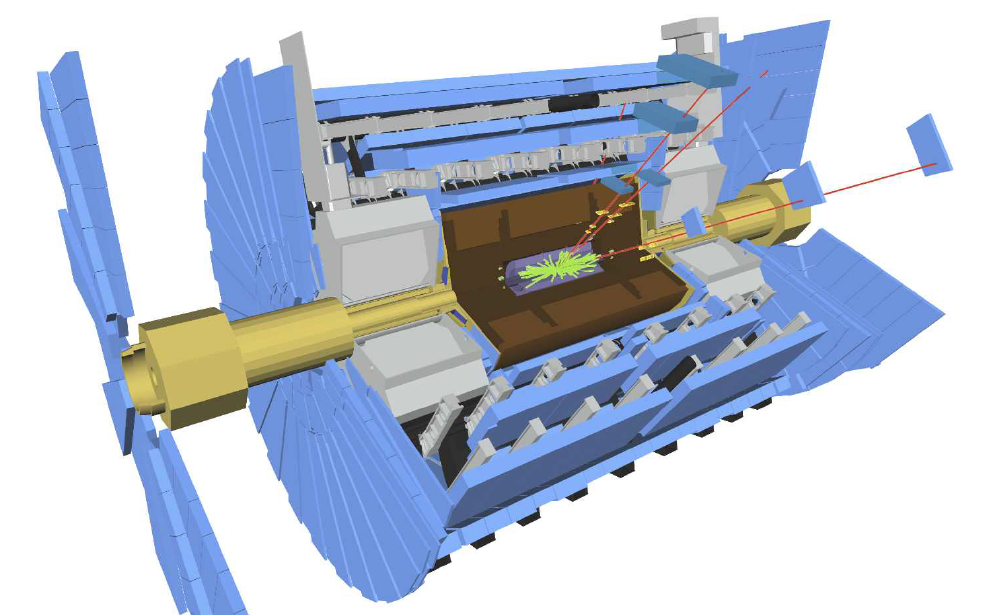
\includegraphics[width=.75\textwidth]{MCSample/simulation}
\caption{An event display made with VP1. VP1 is a viewing software made specifically for ATLAS which stands for Virtual Point 1, since ATLAS is situated at Point 1 of the LHC ring. It shows a Higgs boson decaying into four muons (shown in red). Inner detector tracks are in green, and energy deposited in the calorimeter by the muons is shown in yellow.}
\label{fig:simulation}
\end{figure}

\section{Digitization}
The ATLAS digitization software converts the hits produced by the core simulation into detector responses i.e ``digits''. In real events a digit is produced when a signal is recorded in a readout channel of the detector~\cite{simulation}.

In addition to the hard scattering digitization, pile-up and any other source of noise must be incorporated. For pile-up simulation, there are also input HIT files for minimum bias events to be overlaid, whose number for each bunch crossing is a function of the luminosity simulated. Moreover cavern background and cosmic muons could influence the simulation.

The ATLAS detector electronic produces data in bytestream format called RawData Objects (RDO) whose size on disk is typically \SI{2.5}{MB\per event} and increases with larger number of \pileup events.

%RDO TRIGGER?

\section{Reconstruction}
\label{sec:recoreal}

Within this section, physics object definition and reconstruction in ATLAS are discussed, focusing on those mainly involved in this analysis. Definitions follow the recommendations from the various Combined Performance (CP) groups.

A reconstructed event in ATLAS is an ensemble of signals produced in the detector, which must be processed in order to get particle's property and identification. 

This step is identical for both real data and MC generated events and produces an output file in a Event Summary Data (ESD) and Analysis Object Data (AOD) form. 

Within this section, physics object definition and reconstruction in ATLAS is described, focusing on those mainly involved in the \mph analysis. Definitions follow the recommendations from the various Combined Performance (CP) groups.



\subsection{Photons}
\label{photons}
\subsubsection{Reconstruction}
Photons are reconstructed from clusters in the electromagnetic calorimeter measured in projective towers but uses information from the Inner Detector as well. These towers are portions of the second layer of the calorimeter of $N_1 \times N_2$ cells in the $\eta-\phi$ plane. Photons and electrons (positrons) signature and energy deposits are very similar in the EM calorimeter. That's why information from ID to discriminate them are essential: a photon would not produce any track since the ID is sensitive only to charged particles. A cluster with no tracks associated is classified as a \emph{unconverted} photon since it was produced in a primary vertex it is straight revealed by the EM calorimeter. A \emph{converted} photon, instead, is produced in a primary vertex, it generates a electron-positron pair in a secondary vertex within the ID whose tracks can be associated to the cluster.

The reconstruction process starts from a \emph{sliding-window} algorithm. It looks for the optimal clusters starting from windows of $3\times5$ cells, or $0.025\times0.025$ in $\eta-\phi$, for unconverted photons and $3\times7$ cells ($0.175\times0.175 \, \eta\times\phi$) for converted ones, in the barrel region of the EM calorimeter, whose energy deposited is greater than \SI{2.5}{\gev}. In the endcap, clusters of size $5\times5$ are used for all photon candidates.

%In order to identify an object as a photon or electron, tracks information is necessary. The tracking algorithm, Gaussian Sum Filter (GSF), reconstructs tracks by fitting points within the pixel detector and first layers of SCT and extrapolates informations gathered to outer layer of the ID and into the EM calorimeter. The algorithm also carefully trests the energy losses due to bremsstrahlung. Working along with the tracking algorithm, the vertexing algorithm analyses and classifies the interaction vertices and requires that a track points toward the center of the cluster whithin a $0.05\times0.05$ $\eta\times\phi$ window. Clusters with no matching tracks are classified as unconverted photons. Otherwise it is reconstructed as a converted photon or an electron.

Any noisy or sporadic noisy channel can sometimes produce a signal with transverse momentum larger than \SI{2.5}{\GeV }and give rise to a sliding window cluster~\cite{photons}. In order to identify these bad quality or fake clusters coming from instrumental problems cleaning cuts are applied on photon candidates. A photon is flagged as bad if it contains or edges dead/masked cells.

\subsubsection{Identification}
\begin{figure}[tp]
\centering
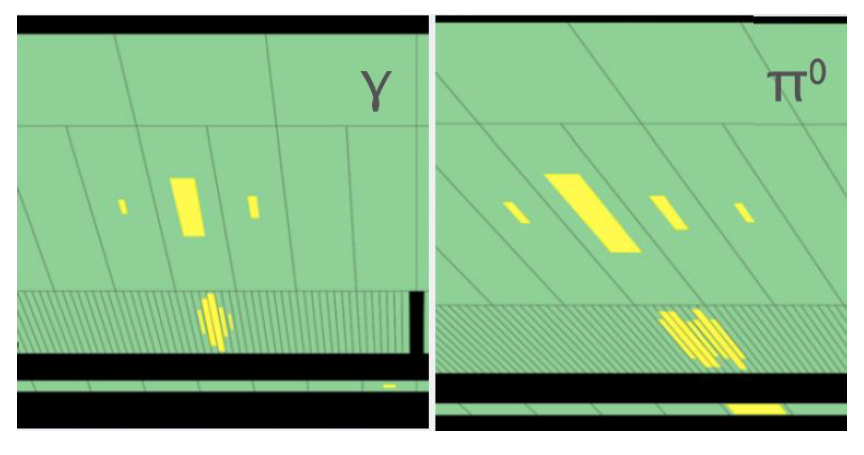
\includegraphics[width=.65\textwidth]{MCSample/pizerogamma}
\caption{Discrimination between a single photon and two collimated photons from a \pizero decay in the the ATLAS EM calorimeter. From the bottom to the top the strip, middle and back layers are visualized.}
\label{pizerogamma}
\end{figure}

Once a list of candidate photons has been made, we have to discriminate between real photons and hadronic jets containing high \pt \pizero, as shown in \Fig{\ref{pizerogamma}}. Identification is based upon the information from the strip and middle layers of the EM calorimeter.

Two working points are defined for photons: loose and tight depending on which cuts a photon passes based on shower shapes measured in strips and middle layers of the EM calorimeter together with hadronic leakage. The differences observed between data and MC in the discriminating variables are measured comparing the shower shape distributions in data and MC, and parametrized as simple shifts. Instead, three working points which are loose, medium and tight, have been defined for electrons. Details on photons selection criteria can be found in \cite[Sect. 4]{photons}.

Identification efficiency is computed with three different data-driven methods presented in~\cite{photons}: the matrix method, electron extrapolation and measure of radiative photons from  \mbox{\Zboson\rarrow\ellell$\gamma$} decays whose comparison is given in \Fig{\ref{fig:phID}} for converted photons. Tight photons efficiency identification is expected to be greater than \SI{90}{\percent}.

\begin{figure}[pt]
\centering
\includegraphics[width=0.65\textwidth]{MCSample/phID}
\caption{Comparison of the data-driven mesurements of the identification efficiency for converted photons as function of \et in the region \SIrange{10}{1500}{\gev}, for the pseudorapidity interval \AetaRange{0.6} using data collected in 2015-2016.}
\label{fig:phID}
\end{figure}

\subsubsection{Isolation}
\label{sec:phisolation}
\begin{figure}[tp]
\centering
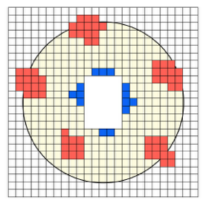
\includegraphics[width=0.33\textwidth]{MCSample/topoetcone40}
\caption{The algorithm which fills TopoEtCone40 variable in action: from the $R=0.4$ cone (yellow) a $5\times7$ rectangle is removed, energy deposited is computed among the \topo~within the cone (orange) and the \pt-leakage (blue) is subtracted.}
\label{topoetcone40}
\end{figure}

Usually the isolation of a particle is expressed in terms of $E_\textup{T}^{\textup{iso}}$ which computes the transverse energy measured in the calorimeter cells (\topo) whithin a cone of given radius around the candidate. A track isolation $p_\textup{T}^{\textup{iso}}$variable can be defined as well.

In the above mentioned cone, an algorithm sums up the energies of the \topo~with energy deposits above a certain threshold~\cite{photonsISO}. The contribution of the photon itself, in a $5\times7$ cells area around the cone axis, and from the underlying evens and \pileup is  subtracted and the \pt-leakage, i.e. photon energy escaped from the area previously identified, is taken into account. Then the total energy in the cone is computed and the variable storing this information in our analysis is ``TopoEtCone40'' which contains the energy evaluated in a cone of radius $R=0.4$. Therefore a photon is considered isolated if ``TopoEtCone40''remains below a certain threshold, i.e. $\text{TopoEtcone40} < 0.022\pt^\gamma + \SI{2.45}{\GeV}$ and $\text{ptcone20}/\pt^\gamma<0.05$. A visual representation of the process described is given in \Fig{\ref{topoetcone40}}.

Isolation efficiency is computed to be greater than \SI{90}{\percent} for $\et^\gamma$ greater than \SI{100}{\gev}~\cite{photonsISO}.


\subsection{Missing transverse momentum*}
\label{sec:met}
\subsubsection{Reconstruction}

An intuitive definition of missing transverse momentum (\met) is the momentum inbalance in the transverse plane. A non-zero inbalance, must suggest the presence of missing energy since this plane is boost-invariant and energy must be conserved. Indeed we can state something only about transverse energy since the parton momentum in the beam direction before the collision is unknown.

The true \met is given simply by neutrinos and non interacting particles, but also there are other sources such malfunctioning detector region or its finite coverage so that a reconstructable particle becomes invisible. This is particularly relevant for this analysis when we look for to \emph{non}-interacting particles such DM particles.

Here we refer to \met as a scalar quantity with \met. For a detailed explanation of the  to the calibration and reconstruction of this quantity refer to \cite{met}.

The \met calculation used in this analysis is based on all reconstructed and calibrated physics objects. In the transverse plane the scalar energy and the corresponing azimuthal angle are given by:
\begin{gather}
\label{eqn:met}
	\met=\sqrt{(E_x^\textup{miss})^2+(E_y^\textup{miss})^2}\\
	\phi^\textup{miss}=\arctan\big({E_y^\textup{miss}/E_x^\textup{miss}}\big)
\end{gather}

The single components $E_i^\textup{miss}$, ($i=\{x,y\}$), in equation \ref{eqn:met} is given by:
\begin{equation}
	E_i^\textup{miss}=E_i^\textup{miss,$e$}+E_i^\textup{miss,$\gamma$}+E_i^\textup{miss,$\mu$}+E_i^\textup{miss,$\tau$}+E_i^\textup{miss,jets}+E_i^\textup{miss,Soft}
\end{equation}

Each term is calculated as the negative sum of the reconstructed objects, projected on the transverse plane and reverting the corresponding \pt. The ``Soft'' term is calculated from energy deposits or tracks which are not matched to selected hard objects. 

There are several computation of \met. The one this analysis is based on is the ``Track Soft Term'' (TST) as recommended by ATLAS CP groups, calculated from the tracks from the primary vertices that are not matched to selected hard objetcs providing a stronger measurement against \pileup~\cite{met}.

\section{EXOT6 Derivation}
\label{sec:derivation}
During the \RunTwo ATLAS has developed a ``Derivation Framework'', by proposal by the Analysis Model Study Group (AMSG), which works on the principle that analyzers need to be able to run over their data sample frequently. For this purpose the derivation framework provides the offline software tools and structures to work on data in a very simple way~\cite{twiki:DAOD}. 

Unlike in \RunOne, when derivation was made by users, this production is now made centrally by the ATLAS production services, even if it can be run locally as in our case, avoiding difficulties in cross-team analyses due to differences in the formats and in reading the output file.

Derivations are made from the reconstructed data via four operations:
\begin{enumerate}
\item skimming: the removal of entire events,
\item thinning: when removing the whole object in an event, but keeping the rest of it 
%(for instance an electron is totally removed while other object remains),
\item slimming: information removal from objects, while keeping the rest of it 
%(i.e. only certain object information ,such its transverse momentum. are removed but the object still remains in the event),
\item augmentation: adding informations not found in the input data.
\end{enumerate}

Therefore the derivation framework selects only the relevant data for a specific analysis, from all ATLAS data collected. This functioning is well explained in the sketch shown in \Fig{\ref{fig:derivation}}.

For this analysis a specific derivation called ``EXOT6'' has been implemented and the following skimming selection was applied:
\begin{itemize}
\item Events must pass one out of several trigger request, including the \verb!HLT_g140_loose! which this analysis is based on;
\item Events must have one loose\footnote{see \Sect{\ref{photons}}} photon with $\pt\ge\SI{80}{\gev}$ or one loose electron with $\pt\ge\SI{100}{\gev}$.
\end{itemize}

As final step a RooT::NTUPLE file was produced in which events are once again selected following the recommendation by the Combined Performance groups. The analysis code is based on SUSYTools-00-08-20 based on AnalysisBase 2.4.28. Details on object definition and kinematic cuts performed in the SUSYTools code are given in~\cite{twiki:SUSYTools}.


\begin{figure}[t]
\centering
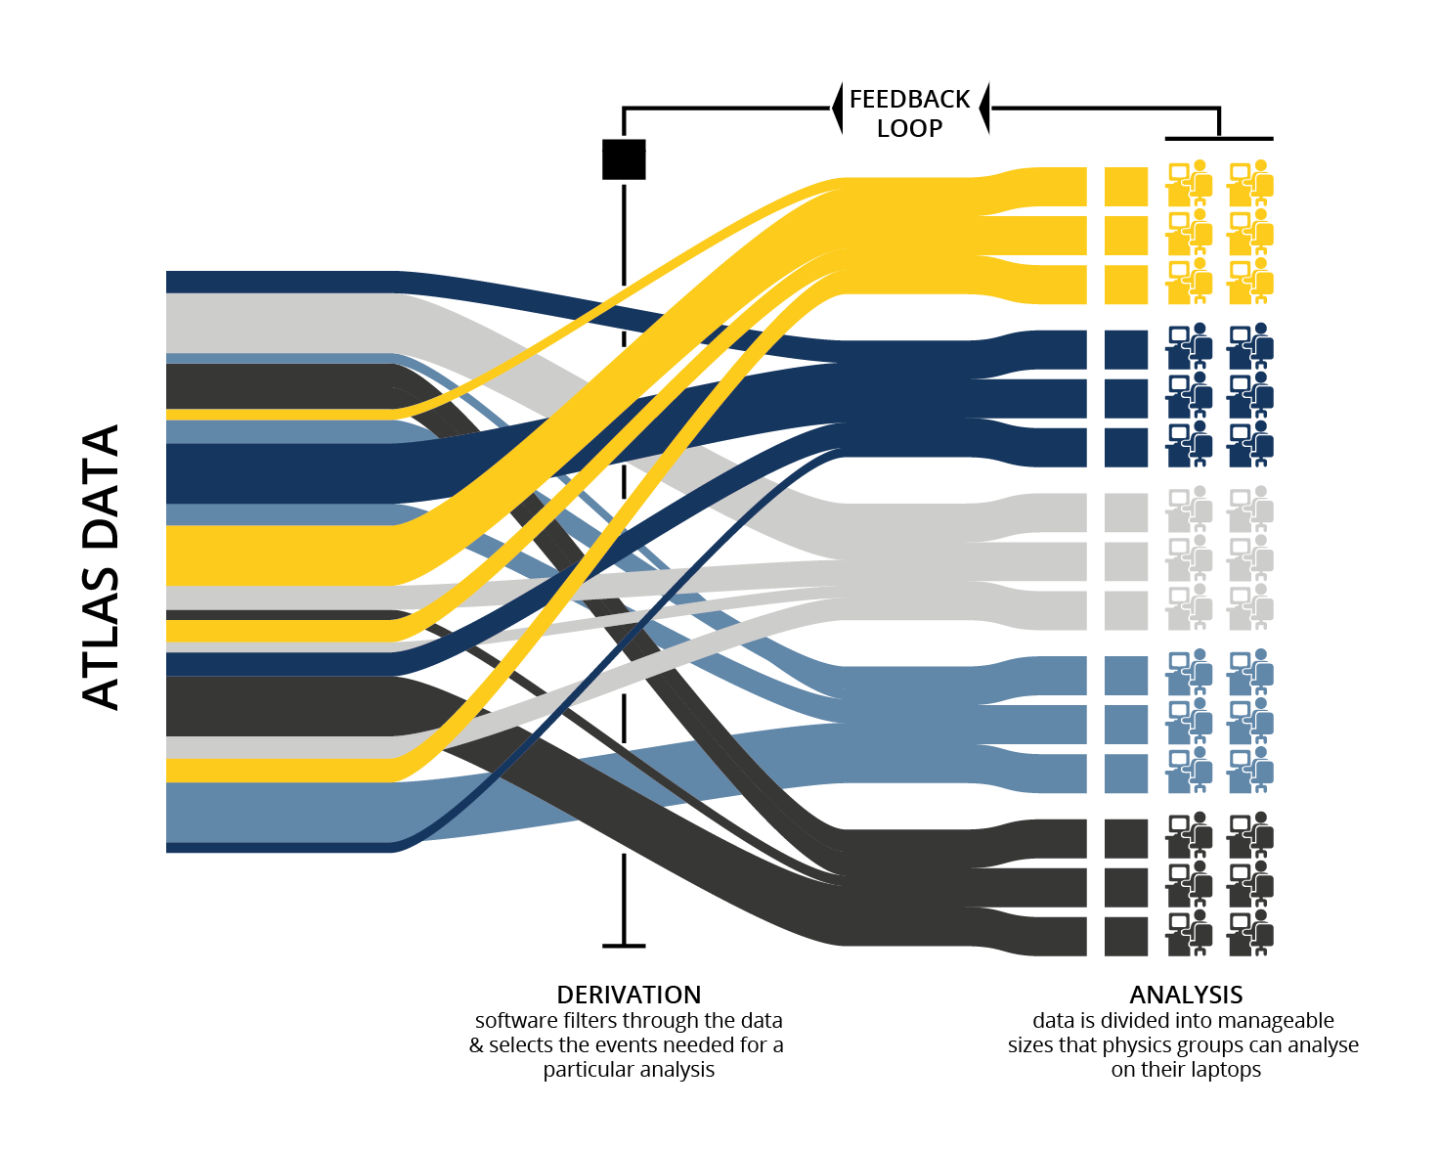
\includegraphics[width=.55\textwidth]{MCSample/Derivation}
\caption{Sketch of how the derivation code works for ATLAS data. Each single event from the whole amount of ATLAS data contains different characteristics that the derivation code depending on the analysis performed.}
\label{fig:derivation}
\end{figure}
















\clearpage
\thispagestyle{empty}
\chapter{Fundamentals of the \mph analysis}
Large missing transverse momentum (\met) signature can be sign of evidence of new physics, such as the indirect detection of dark matter.

At LHC we can produce DM particles if they interact with Standard Model particles. A possible candidate to be a constituent of dark matter in universe is given by a weakly interactive mass particle (WIMP) which interacts with SM particles with a strenght similar to the weak interaction so it leaves no track on the detector. Missing transverse momentum can only be measured  if other particles are produced in the collision, for instance a detectable object such jets or photons, in order to tag the WIMP particle production. This kind of analysis are called Mono-X, for one selects events with a single object in final state. In the \mph analysis we are looking for a single high energy photon and large missing transverse momentum signature. The \mph analysis is characterized by a relative clean final state thanks also to a small set of SM processes that produces the same outcome.

For the analysis we are using data collected during 2015 and 2016 with the ATLAS detector, corresponding to an integrated luminosity of $36.4$ \ifb.

In this chapter after giving a definition of signal and control regions describing the kinematic cuts used to constrain data I present the result for a background only analysis. I give also a brief evaluation of the raise of systematic uncertainties.

\section{Event selection}
In the context of this \mph analysis several Conotrol Regions (CRs) enriched with the corresponding dominant background in order to extract their normalization on data and a Signal Region (SR) in which eventual signal could be found.

\subsection{Selection in Signal Region}
Events in SR are preselected required by the following property:
\begin{description}%MAGARI CAMBIALO CON UNA DESCRIPTION
\item [Data quality] Data are considered good for physics if belonging to the Good Run List (GRL). They have to be collected in periods in which optimal detector functioning and stable beams were provided;
\item [Trigger acceptance] Events selected must pass the  \verb!HLT_g140_loose! trigger, which {\itshape I think} is a trigger used to detect events with large \met; 
\item [Vertex quality] We take into account events having a primary vertex reconstructed with two associated good-quality tracks with \pt $\ge 400 \,$\MeV and \AetaRange{2.5}
\item [Jet cleaning] Jets tagged with {\itshape BadLoose} (la [38] della nota) in events in which they overlap with photons or leptons with \pt$> 20$ \GeV or not coming from hard scattering are rejected.
\end{decription}

After the preselection Candidates in SR are selected with the following kinematic cuts. In order to populate the region with \gmet events, we consider an event to be part of this region if:
\begin{itemize}
\item we compute \met $ \ge 150 $ \GeV;
\item we get one loose photon with \pt $ \ge 150 $ \GeV $\,$ with a pseudorapidity cut in \etaRange{1.52}{2.37} to cut ot the calorimeter crack region and \AetaRange{1.37}
\item \met significance is found to be above $8.5$ \GeV$^{-\frac{1}{2}}$
\item the leading photon is isolated, so that we select events characterized by $ \text{TopoEtcone40} \le 2.45$ \GeV$ + 0.022 \, $\pt \GeV. By this we ensure that in a cone with radius \DeltaRdef $ = 40$, centered in the photon track, all the Topo Clusters have less energy deposited than the one defined above.
\item photon track and \met doesn't overlap, requiring $\Delta\phi_{\gamma - \met} \le 0.4$
\item photon pointing along z coordinate wrt the identified primary vertex must no be larger than $250 \, mm$
\item there is at most one {\itshape good} jet. Even if the analysis is called \mph we take into account events even if they contains a jet, if not we could reject too much statistics as it will be clear in validation plots in section {\bfseries which hasn't been written yet}. Moreover we take only jets such that $\deltaphijetgamma \ge 0.4$

\end{itemize}

In the following section I'm going to deal with all the sources of interference that could affect the SR describing the background processes.

\section{Background estimation}
Alongside the eventual signal coming from unknown ph\oe nomena many other SM processes could pass the cuts defined for the SR ending up being tagged in a wrong way as new physics. We call them background signal, i.e. predictable events that lead to the same signature we are looking for when producing DM particles from \pp scattering.

In other words reasons for events of background can be ascribed to:
\begin{itemize}
\item properly reconstructed SM events which have the same final state as the signal we are looking for;
\item badly reconstructed events in which one (or more) particle are mistaken for photons or they are not reconstructed at all.
\end{itemize}

For the \mph analysis the following background processes were considered.
\begin{itemize}
\item \znng where the two neutrinos produce high \met in the detector. This is the dominant, other than the only irreducible, background as one can see from plots.
\item \wg in which all possible leptonic decay mode of \Wboson are gathered. Here $\ell$ can be an electron being missed or reconstructed as a photon, a muon being missed as well, or a $\tau$ lepton which can decay via hadrons and reconstructed as jet or via leptons and being missed in the detector.
\item \zg where, once again, I am considering all possible leptonic decays for the \Zboson where leptons end up in the same records as in the \Wboson case
\item \gj events in which a jet or photon misreconstruction leads to fake \met.
\item All kind of processes where a jet can fake a photon including:
  \begin{itemize}
  \item double neutrino decay of \Zboson combined with a jet,
  \item leptonic decay of \Wboson along with a jet. If an electron is involved it could fake a photon as well, while we are keeping the jet as pure object for passing SR cuts.
  \end{itemize}
\end{itemize}

In order to quantify the amount of background events in SR, several Control Regions (CRs) are defined which are assumed to be free of signal contamination. Each of them is defined reverting one or more constraints for the SR to enrich every region with a given background process so that they are characterized by a pure dominant process among the others. This provides also ortogonality of a region to one another and their statistical independence.

Events in CRs are simulated via Monte Carlo samples whose prediction must be fitted on data, to get a more reliable estimate of background in SR. This procedure will be explained in detail in section {\bfseries to be written}. A special procedure must be carried out for electron and jets faking photons. In this work results in all the regions for these sources have been taken from previous analysis. However this kind of background cannot be quantified like the previous ones because it is due to some detector mistakes in reconstruction.



\subsection{Transfer factor technique and normalisation of background}
In CRs the respective dominant background can be controlled by comparing MC samples to data. Initial predictions of background in a certain CR must be scaled to observed data in that region, using a normalization factor ($k_{i}$) which is usually computed by a numerical fit by the HistFitter software framework. Usually this procedure is referred as an extrapolation from CRs to SR.

One can define a Trasfer Factor by a mere ratio between MC prediction in SR and MC prediction in a CRs, both unnormalized (raw), and the estimate of the number of events in the signal region for the $i$-th process could be written in terms of event observed in the CRs as:
\begin{equation}
  \label{eqn:TF}
  N_{\textup{est},i}(\text{SR}) =  N_{\textup{obs},i}({\text{CR}}) \times \left[\frac{\text{MC}_{\textup{raw},i}(\text{SR})}{\text{MC}_{\textup{raw},i}(\text{CR})} \right]
\end{equation}

The proper normalization factor is defined as the ratio between events observed and expected in the CRs and equation \ref{eqn:TF} can also be rewritten:
\begin{equation}
  N_{\textup{est},i}(\text{SR}) = k_{i}\times\text{MC}_{\textup{raw},i}(\text{SR})
\end{equation}

By this factor the PDF of every region is rescaled everywhere in the parameter space. Indeed the analysis strategy performed by HistFitter shares the same parameters in all region so that any information found in a single region can be brought to the others.

The advantage of using this procedure is that that systematic uncertainties common to the numerator and the denominator of the TF, such as the uncertainty on luminosity, on the predicted background processes can be canceled at first order in the extrapolation.

\subsection{Definition of Control Regions}
There are four CRs definded in order to extrapolate information on background in Signal Region. In this section a brief definition and differences in kinematic cuts are descrbed.

\begin{description}
\item [One muon CR] In this region one selected muon is requested, kinematic cuts on \pt and \met are the same of those in SR. Here, however, \met is computed in a different way that is the muon energy is added to this variable, so we can treat it as an invisible particle in order to ensure that \met distribution is similar to the one in SR. This region extracts the normalization $k_W$ for \wg background.
\item [Two muon/electron CR] Similarly to the One muon, here we add to \met both muon/electron contribution to \met. Here two selected muons/electrons are required. we can also add a constrain to the invariant mass of the di-lepton to be greater than 20 \GeV\, and less than 1 \TeV \, to avoid any BSM $Z\gamma$ resonances. Moreover we don't require the cut on \met significance. These regions get $k_Z$ for the dominant background \zg in this region which applies via branching ratio to the \znng process.
\item [Photon jet CR] Here kinematic cuts on \met are lowered. We require \met to be in 85 - 110 \GeV\, range to enrich this region of \gj background because in this energy range, probability to have fake \met from jets is higher. To avoid signal contamination we set $\Delta\phi_{\gamma - \met} \le 3.0$ so that we prevent {\itshape back-to-back} signal events to fall in this region. This region, defined in \RunTwo, constrains the normalization for \gj background to get a $k_{pj}$ normalization factor.
\end{description}

{\itshape A priori} a one electron CR could have been defined as well. Nevertheless the one muon CR has enough statistic to constrain the normalization on \Wboson$\gamma$.  This kind of region would have been more difficult to manage even just because electrons could be reconstructed easily as photons which not happens for muons being detected far away in the detector from photons increasing the number of \gj events contamination. In the analysis carried out in [nota di supporto] one evince that no improvement on $k_W$ error can be seen, instead there is a raise of $k_{pj}$ error due to furhter background contamination.

As mentioned earlier fake photons from electrons and jets enter the fit as given values and it is not constrained by any region. They have been estimated via data driven tecniques in other analysis.

\section{Results for a background-only fit}
{\bfseries To be written}

\clearpage
\thispagestyle{empty}
\chapter{Interpretations of the results}

\lettrine{D}{}ata yield in \SI{36.4}{\ifb}, presented in the previous chapter, are in agreement with prediction of the SM. This chapter quantifies this level of agreement introducing appropiate test statistics allowing to set model independent, regardless of the model considered, and model dependent, within the Minimal DM model, upper limits.

\section{The profiled likelihood ratio}
In \Sect{\ref{sec:likelihood}} the Likelihood function was defined as a function of the POI $\mu$~\cite{Cowan}.
A very common procedure to establish discovery (or exclusion) in particle physics is based on a likelihood ratio as a test statistic. Indeed, to test an hypothesized value of $\mu$ the \emph{profiled likelihood ratio} which is used as the principal statistical parameter in this analysis, has been considered.
\begin{equation}
  \lambda(\mu) = \frac {\mathfrak{L}(\mu,\hat{\hat{\theta}})}{\mathfrak{L(\hat{\mu},\hat{\theta})}}
  \label{eqn:profiled}
\end{equation}
where the numerator, $\hat{\hat{\theta}}$ conditional maximum-likelihood estimator (MLE) of $\theta$, or the value which maximies $\mathfrak{L}$ for a given $\mu$ (therefore, it is a function of $\mu$, and the denominator is the maximized, unconditionally by fixing no parameters, likelihood function. \Eqn{\ref{eqn:profiled}} is a rescaling of the likelihood function: 

\subsection{The $t_\mu$ test statistic}
The profiled likelihood ratio $\lambda(\mu)$ is constrained to vary between 0 and 1 so that it is useful to define the corresponding $\tmu$ statistic as 
\begin{equation}
  t_{\mu} = -2 \log{\lambda(\mu)}
\end{equation}
which can be used to build a statistic to measure the discrepancy between data and the hypothesis where higher value of $t_{\mu}$ correspond to higher disagreement. The \p can also be evaluated, and its correspondance to $t_{\mu}$ is pointed out in \Fig{\ref{pvalue}}, as:
\begin{equation}
 p_{\mu}=\int_{t_{\mu,\textup{obs}}}^\infty f\left(t_\mu \vert \mu\right) dt_\mu
 \label{eqn:pdatmu}
\end{equation}

where $t_{\mu,\textup{obs}}$ is the value of $t_\mu$ observed from data and $f\left(t_\mu \vert \mu\right)$ is the probability density function of $t_\mu$ under the assumption of the POI value $\mu$. One can often assume that presence of new signal can only increase the mean event rate, which for a counting experiment can be evaluated as $E[n] = \mu s + b$ where $s$ are the signal events and $b$ is the background, so that we can consider parameter $\mu$ as positive so that an alternative test statistic $\tilde{t}_\mu$ can be defined. For a model in which $\mu>0$, if one finds that $\hat{\mu}<0$, the best level of agreement must be for $\mu=0$.

Note that $f\left(t_\mu \vert \mu\right)$ in \Eqn{\ref{eqn:pdatmu}}, like all the $f$ distribution in this Section, is unknown, because we miss the real POI which is crucial to its determination. According to Wilks' theorem, the distribution of $f(t_\mu \vert \mu)$ is known in the case of a large statistics an it follows a one-degree of freedom (in case of one POI) $\chi^2$ distribution, regardless of the values taken by the nuisance parameters, see~\cite[\Sect{3}]{Cowan}, so that $f$ is expressed in term of certain asymptotic formul\ae~ in the limit of large samples. Alternatively one can obtain it by performing several pseudo-experiment, i.e. \emph{toys}, to get the right distribution expression even if they're always time expensive.

\begin{figure}[tp]
\centering
\subfloat[][]
{\includegraphics[width=.4\textwidth]{monophoton/pvaluea}}
\subfloat[][]
{\includegraphics[width=.416\textwidth]{monophoton/pvalueb}}
\caption{(\emph{a}) Relation between \p and $t_{\mu,\textup{obs}}$. (\emph{b}) Relation between the significance $Z$ and \p for a gaussian distribution $\varphi(x)$.}
\label{pvalue}
\end{figure}

\subsection{Test statistics for discovery and exclusion fit}
Without any observed excess of events in one or more SR(s), two methods set exclusion
limits on specific signal models. These two fit strategies, complementary to the background only fit described {\bf above}, are the discovery fit, or model-independent and the exclusion fit model-dependent. Both fit are used to set upper limits on the POI, i.e. the number of events in case of discovery and the visible cross section for exclusion, by varying its value whithin a certain range and then interpolating for which POI value one finds \SI{95}{\percent} exclusion. For this reason, setting an upper limit is also called \emph{hypotest inversion}.

\subsubsection{The $q_0$ test for discovery of a positive signal}
When searching for new physics phenomena typically one would put constraints on potential new physiscs. Indeed, in a discovery fit the purpose is to set model-independent \SI{95}{\percent} CL upper limits on the number of Beyond Standard Model (BSM) events in SR. For no signal model in particular anyone can estimate the number of signal events predicted in a particular SR, in our case the already defined ``fiducial region'', and see wether a certain model has been excluded by current data or not.

In this scenario rejecting the $\mu = 0$ hypothesis leads to the discovery of a new signal.  An appropriate test, the $q_0$ test statistic, is therefore defined as follows:
\begin{equation}
q_0=
\left\{
\begin{aligned}
-2\log{\lambda(0)}\quad &\text{if}\quad \hat{\mu}\ge0\\
 0 \qquad&\text{if}\quad \hat{\mu}<0
\end{aligned}
\right.
\end{equation} 

Data shows lack of agreement with the background only hypothesis ($\hat{\mu}=0$), only if $q_0\ne0$. Using the observed value of $q_0$ one can quantify the level of disagreement between the data and the null hypothesis not so much unlike for the $t_\mu$ case:
\begin{equation}
 p_{\mu}=\int_{q_{0,\textup{obs}}}^\infty f\left(q_0 \vert 0\right) dq_0
 \label{eqn:pdaq0}
\end{equation}

\subsubsection{The $q_\mu$ test for model dependent upper limits}
This fit strategy is used with the objective of studying a specific signal model. Again, with no relevant excess of events proved by the background only fit exclusion limits can be performed for    setting upper limit on the visible cross section of the model being tested. The signal sample must be added to every CRs and not only in the SR, in order to take into account any posssible signal contamination in the CRs. Note that this test is useful even in case of excess of events for which can be used to measure properties such as the signal strength.

Like for the model independent fit, a suitable test statistic can be defined for the model independent fit as well, in a very similar way. However, now the null hypothesis is the signal+background coexisting in the SR because a signal is supposed to be tested against the back. Therefore the $q_\mu$ test statistic is defined as:
\begin{equation}
q_\mu=
\left\{
\begin{aligned}
-2\log{\lambda(0)}\quad &\text{if}\quad \hat{\mu}\le\mu\\
 0 \qquad&\text{if}\quad \hat{\mu}>\mu
\end{aligned}
\right.
\end{equation} 
Once again the relation between $q_\mu$ and the \p is straighforward:
\begin{equation}
 p_{\mu}=\int_{q_{\mu,\textup{obs}}}^\infty f\left(q_\mu \vert \mu\right) dq_\mu
 \label{eqn:pdaqmu}
\end{equation}

\subsection{Experimental sensitivity}
\label{sec:sensitivity}
To characterize the sensitivity of an experiment, the significance obtained from a single dataset is irrelevant. The expected (or median) significance which allows to reject different values of $\mu$ is more useful. In a discovery analysis one would like to know the median significance with which one would reject the background-only null hypothesis and for exclusion the median with which one rejects a nonzero value of $\mu$.

The median significance is obtained by replacing the ensamble of simulated data set with a single representative one, the so-called Asimov data set which it is easy to obtain the median values of $q_0$ and $q_\mu$.

The sensitivity of an experiment is illustrated in \Fig{\ref{fig:medianq}} which shows the PDF for $q_\mu$ assuming an observed (tested) value of $\mu$ and an expected value of $\mu'$ retrieved from certain asymptotic formul\ae~ valid in the case of large samples~\cite{Cowan}. Analogous consideration can be made for the discovery analysis by replacing $q_\mu$ with the corresponding $q_0$. The sensitivity of an experiment can be characterized by giving the \p corresponding to the median $q_\mu$, assuming $\mu=\mu'$. 

When the distribution of the strenght parameters $\mu'$ gets shifted to higher values, so does the median $q_\mu$. From \Eqn{\ref{eqn:pdaq0}} and \Eqn{\ref{eqn:pdaqmu}} it is clear that \p is pushed towards lower values. Now the hypotest inversion is finally revealed. What the fitting procedure achieved is to scan several values of $\mu$ and evaluate the median \p assuming $\mu'$. The computed upper limit is therefore the value of $\mu$ for which \p gets under the threshold of \num{0.05}.

In the context of exclusion limits, the $\cls$ statistic is mostly used replacing the \p. $\cls$ being derived from the \p is defined as:
\begin{equation}
	\cls=\frac{\text{p-value}(H_0)}{1-\text{p-value}(H_1)}
\end{equation}

Upper limits are then set for the value when $\cls$ is computed to be below the $0.05$ threshold.

\begin{figure}[pt]
\centering
\includegraphics[width=0.5\textwidth]{interpretations/medianq}
\caption{Representation of the situation described in \Sect{\ref{sec:sensitivity}}. The observed distribution $f\left(q_\mu \vert \mu \right)$ is overlapped with the median $f\left(q_\mu \vert \mu' \right)$ given by the asimptotic formul\ae~ according to which it has the form of an half chi squared distribution. The median $q_\mu$ is computed assuming the alternate value $\mu'$ and the result is used to calculate the \p for distribution $f\left(q_\mu \vert \mu \right)$.}
\label{fig:medianq}
\end{figure}

\section{Model-independent limit}
The model-independent, discovery, fit purpose is to set upper limit on the number of BSM events that can be found in the SR. This can be achieved by counting the excess of events yield on the basis of a bogus signal model that is a single bin histogram with the bin value at 1. In this case the strenght parameter $\mu$ assumes the meaning of number of events, and upper limits are given in terms of that. By rescaling with luminosity via \Eqn{\ref{eqn:Nevents}} one can obtain the corresponding upper limit on the visible cross section $\sigma_\textup{vis}=\sigma_\textit{th}\times A\times\epsilon \equiv N/L$ where $\sigma_\textit{th}$ is the theorical cross section. Results are reported in \Tab{\ref{table.results.exclxsec.pval.upperlimit.SR}}.


\begin{table}[pt]
\centering
%\setlength{\tabcolsep}{0.0pc}
\begin{tabular}{ccc}
\noalign{\smallskip}\toprule\noalign{\smallskip}
L [\ifb]&$\rm \sigma_{\rm vis}^{\rm obs}$~[fb] &$\rm \sigma_{\rm vis}^{\rm exp}$~[fb] \\
\noalign{\smallskip}\midrule\noalign{\smallskip}
%%
$36.4$&$5.91$ &${ 8.86 }^{ +3.31 }_{ -2.39 } $ \\
\noalign{\smallskip}\midrule[.2pt]\noalign{\smallskip}
$120$&$-$ &${ 2.69 }^{ +1.00 }_{ -0.73 } $ \\
\noalign{\smallskip}\noalign{\smallskip}
$3000$&$-$ &${ 0.108 }^{ +0.040 }_{ -0.029 } $ \\
 
 
\noalign{\smallskip}\bottomrule\noalign{\smallskip}
\end{tabular}
\caption[Breakdown of upper limits.]{
Left to right:  First column reports the integrated luminosity used, then \SI{95}{\percent} CL upper limits on the visible cross section observed
followed by the expected
reporting the $\pm 1\sigma$
excursions are given. 
Expected limits are given the absence of new physics.
First row of the table reports the result achieved in this work and found to be in good agreement with thise published in~\cite{paperMP}, and below the solid line
outlooks at high luminosity is given.
\label{table.results.exclxsec.pval.upperlimit.SR}}
\end{table}
%

%\section{prova}
%\begin{figure}[tp]
\centering
{\fontfamily{phv}\selectfont  
\small
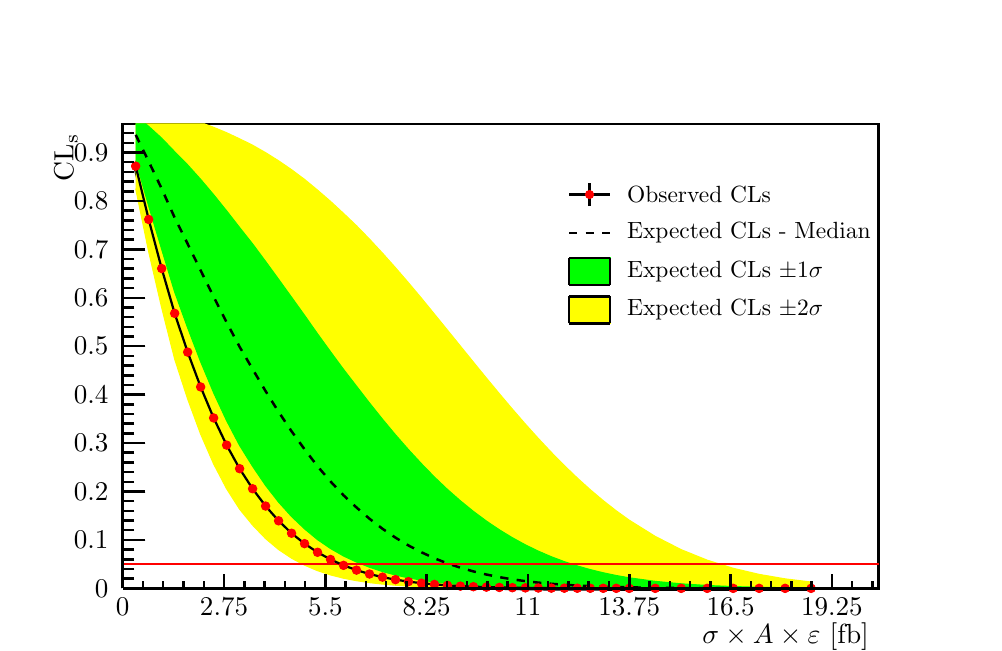
\begin{tikzpicture}[scale=0.6]
\pgfdeclareplotmark{cross} {
\pgfpathmoveto{\pgfpoint{-0.3\pgfplotmarksize}{\pgfplotmarksize}}
\pgfpathlineto{\pgfpoint{+0.3\pgfplotmarksize}{\pgfplotmarksize}}
\pgfpathlineto{\pgfpoint{+0.3\pgfplotmarksize}{0.3\pgfplotmarksize}}
\pgfpathlineto{\pgfpoint{+1\pgfplotmarksize}{0.3\pgfplotmarksize}}
\pgfpathlineto{\pgfpoint{+1\pgfplotmarksize}{-0.3\pgfplotmarksize}}
\pgfpathlineto{\pgfpoint{+0.3\pgfplotmarksize}{-0.3\pgfplotmarksize}}
\pgfpathlineto{\pgfpoint{+0.3\pgfplotmarksize}{-1.\pgfplotmarksize}}
\pgfpathlineto{\pgfpoint{-0.3\pgfplotmarksize}{-1.\pgfplotmarksize}}
\pgfpathlineto{\pgfpoint{-0.3\pgfplotmarksize}{-0.3\pgfplotmarksize}}
\pgfpathlineto{\pgfpoint{-1.\pgfplotmarksize}{-0.3\pgfplotmarksize}}
\pgfpathlineto{\pgfpoint{-1.\pgfplotmarksize}{0.3\pgfplotmarksize}}
\pgfpathlineto{\pgfpoint{-0.3\pgfplotmarksize}{0.3\pgfplotmarksize}}
\pgfpathclose
\pgfusepathqstroke
}
\pgfdeclareplotmark{cross*} {
\pgfpathmoveto{\pgfpoint{-0.3\pgfplotmarksize}{\pgfplotmarksize}}
\pgfpathlineto{\pgfpoint{+0.3\pgfplotmarksize}{\pgfplotmarksize}}
\pgfpathlineto{\pgfpoint{+0.3\pgfplotmarksize}{0.3\pgfplotmarksize}}
\pgfpathlineto{\pgfpoint{+1\pgfplotmarksize}{0.3\pgfplotmarksize}}
\pgfpathlineto{\pgfpoint{+1\pgfplotmarksize}{-0.3\pgfplotmarksize}}
\pgfpathlineto{\pgfpoint{+0.3\pgfplotmarksize}{-0.3\pgfplotmarksize}}
\pgfpathlineto{\pgfpoint{+0.3\pgfplotmarksize}{-1.\pgfplotmarksize}}
\pgfpathlineto{\pgfpoint{-0.3\pgfplotmarksize}{-1.\pgfplotmarksize}}
\pgfpathlineto{\pgfpoint{-0.3\pgfplotmarksize}{-0.3\pgfplotmarksize}}
\pgfpathlineto{\pgfpoint{-1.\pgfplotmarksize}{-0.3\pgfplotmarksize}}
\pgfpathlineto{\pgfpoint{-1.\pgfplotmarksize}{0.3\pgfplotmarksize}}
\pgfpathlineto{\pgfpoint{-0.3\pgfplotmarksize}{0.3\pgfplotmarksize}}
\pgfpathclose
\pgfusepathqfillstroke
}
\pgfdeclareplotmark{newstar} {
\pgfpathmoveto{\pgfqpoint{0pt}{\pgfplotmarksize}}
\pgfpathlineto{\pgfqpointpolar{44}{0.5\pgfplotmarksize}}
\pgfpathlineto{\pgfqpointpolar{18}{\pgfplotmarksize}}
\pgfpathlineto{\pgfqpointpolar{-20}{0.5\pgfplotmarksize}}
\pgfpathlineto{\pgfqpointpolar{-54}{\pgfplotmarksize}}
\pgfpathlineto{\pgfqpointpolar{-90}{0.5\pgfplotmarksize}}
\pgfpathlineto{\pgfqpointpolar{234}{\pgfplotmarksize}}
\pgfpathlineto{\pgfqpointpolar{198}{0.5\pgfplotmarksize}}
\pgfpathlineto{\pgfqpointpolar{162}{\pgfplotmarksize}}
\pgfpathlineto{\pgfqpointpolar{134}{0.5\pgfplotmarksize}}
\pgfpathclose
\pgfusepathqstroke
}
\pgfdeclareplotmark{newstar*} {
\pgfpathmoveto{\pgfqpoint{0pt}{\pgfplotmarksize}}
\pgfpathlineto{\pgfqpointpolar{44}{0.5\pgfplotmarksize}}
\pgfpathlineto{\pgfqpointpolar{18}{\pgfplotmarksize}}
\pgfpathlineto{\pgfqpointpolar{-20}{0.5\pgfplotmarksize}}
\pgfpathlineto{\pgfqpointpolar{-54}{\pgfplotmarksize}}
\pgfpathlineto{\pgfqpointpolar{-90}{0.5\pgfplotmarksize}}
\pgfpathlineto{\pgfqpointpolar{234}{\pgfplotmarksize}}
\pgfpathlineto{\pgfqpointpolar{198}{0.5\pgfplotmarksize}}
\pgfpathlineto{\pgfqpointpolar{162}{\pgfplotmarksize}}
\pgfpathlineto{\pgfqpointpolar{134}{0.5\pgfplotmarksize}}
\pgfpathclose
\pgfusepathqfillstroke
}
\definecolor{c}{rgb}{1,1,1};
\draw [color=c, fill=c] (0,0) rectangle (20,12.2874);
\draw [color=c, fill=c] (2,1.22874) rectangle (18,11.0587);
\definecolor{c}{rgb}{0,0,0};
\draw [c,line width=0.9] (2,1.22874) -- (2,11.0587) -- (18,11.0587) -- (18,1.22874) -- (2,1.22874);
\definecolor{c}{rgb}{1,1,1};
\draw [color=c, fill=c] (2,1.22874) rectangle (18,11.0587);
\definecolor{c}{rgb}{0,0,0};
\draw [c,line width=0.9] (2,1.22874) -- (2,11.0587) -- (18,11.0587) -- (18,1.22874) -- (2,1.22874);
\definecolor{c}{rgb}{0,0,0.6};
\draw [c,line width=0.9] (2,1.22874) -- (2.16,1.22874) -- (2.16,1.22874) -- (2.32,1.22874) -- (2.32,1.22874) -- (2.48,1.22874) -- (2.48,1.22874) -- (2.64,1.22874) -- (2.64,1.22874) -- (2.8,1.22874) -- (2.8,1.22874) -- (2.96,1.22874) -- (2.96,1.22874)
 -- (3.12,1.22874) -- (3.12,1.22874) -- (3.28,1.22874) -- (3.28,1.22874) -- (3.44,1.22874) -- (3.44,1.22874) -- (3.6,1.22874) -- (3.6,1.22874) -- (3.76,1.22874) -- (3.76,1.22874) -- (3.92,1.22874) -- (3.92,1.22874) -- (4.08,1.22874) -- (4.08,1.22874)
 -- (4.24,1.22874) -- (4.24,1.22874) -- (4.4,1.22874) -- (4.4,1.22874) -- (4.56,1.22874) -- (4.56,1.22874) -- (4.72,1.22874) -- (4.72,1.22874) -- (4.88,1.22874) -- (4.88,1.22874) -- (5.04,1.22874) -- (5.04,1.22874) -- (5.2,1.22874) -- (5.2,1.22874)
 -- (5.36,1.22874) -- (5.36,1.22874) -- (5.52,1.22874) -- (5.52,1.22874) -- (5.68,1.22874) -- (5.68,1.22874) -- (5.84,1.22874) -- (5.84,1.22874) -- (6,1.22874) -- (6,1.22874) -- (6.16,1.22874) -- (6.16,1.22874) -- (6.32,1.22874) -- (6.32,1.22874) --
 (6.48,1.22874) -- (6.48,1.22874) -- (6.64,1.22874) -- (6.64,1.22874) -- (6.8,1.22874) -- (6.8,1.22874) -- (6.96,1.22874) -- (6.96,1.22874) -- (7.12,1.22874) -- (7.12,1.22874) -- (7.28,1.22874) -- (7.28,1.22874) -- (7.44,1.22874) -- (7.44,1.22874) --
 (7.6,1.22874) -- (7.6,1.22874) -- (7.76,1.22874) -- (7.76,1.22874) -- (7.92,1.22874) -- (7.92,1.22874) -- (8.08,1.22874) -- (8.08,1.22874) -- (8.24,1.22874) -- (8.24,1.22874) -- (8.4,1.22874) -- (8.4,1.22874) -- (8.56,1.22874) -- (8.56,1.22874) --
 (8.72,1.22874) -- (8.72,1.22874) -- (8.88,1.22874) -- (8.88,1.22874) -- (9.04,1.22874) -- (9.04,1.22874) -- (9.2,1.22874) -- (9.2,1.22874) -- (9.36,1.22874) -- (9.36,1.22874) -- (9.52,1.22874) -- (9.52,1.22874) -- (9.68,1.22874) -- (9.68,1.22874) --
 (9.84,1.22874) -- (9.84,1.22874) -- (10,1.22874) -- (10,1.22874) -- (10.16,1.22874) -- (10.16,1.22874) -- (10.32,1.22874) -- (10.32,1.22874) -- (10.48,1.22874) -- (10.48,1.22874) -- (10.64,1.22874) -- (10.64,1.22874) -- (10.8,1.22874) --
 (10.8,1.22874) -- (10.96,1.22874) -- (10.96,1.22874) -- (11.12,1.22874) -- (11.12,1.22874) -- (11.28,1.22874) -- (11.28,1.22874) -- (11.44,1.22874) -- (11.44,1.22874) -- (11.6,1.22874) -- (11.6,1.22874) -- (11.76,1.22874) -- (11.76,1.22874) --
 (11.92,1.22874) -- (11.92,1.22874) -- (12.08,1.22874) -- (12.08,1.22874) -- (12.24,1.22874) -- (12.24,1.22874) -- (12.4,1.22874) -- (12.4,1.22874) -- (12.56,1.22874) -- (12.56,1.22874) -- (12.72,1.22874) -- (12.72,1.22874) -- (12.88,1.22874) --
 (12.88,1.22874) -- (13.04,1.22874) -- (13.04,1.22874) -- (13.2,1.22874) -- (13.2,1.22874) -- (13.36,1.22874) -- (13.36,1.22874) -- (13.52,1.22874) -- (13.52,1.22874) -- (13.68,1.22874) -- (13.68,1.22874) -- (13.84,1.22874) -- (13.84,1.22874) --
 (14,1.22874) -- (14,1.22874) -- (14.16,1.22874) -- (14.16,1.22874) -- (14.32,1.22874) -- (14.32,1.22874) -- (14.48,1.22874) -- (14.48,1.22874) -- (14.64,1.22874) -- (14.64,1.22874) -- (14.8,1.22874) -- (14.8,1.22874) -- (14.96,1.22874) --
 (14.96,1.22874) -- (15.12,1.22874) -- (15.12,1.22874) -- (15.28,1.22874) -- (15.28,1.22874) -- (15.44,1.22874) -- (15.44,1.22874) -- (15.6,1.22874) -- (15.6,1.22874) -- (15.76,1.22874) -- (15.76,1.22874) -- (15.92,1.22874) -- (15.92,1.22874) --
 (16.08,1.22874) -- (16.08,1.22874) -- (16.24,1.22874) -- (16.24,1.22874) -- (16.4,1.22874) -- (16.4,1.22874) -- (16.56,1.22874) -- (16.56,1.22874) -- (16.72,1.22874) -- (16.72,1.22874) -- (16.88,1.22874) -- (16.88,1.22874) -- (17.04,1.22874) --
 (17.04,1.22874) -- (17.2,1.22874) -- (17.2,1.22874) -- (17.36,1.22874) -- (17.36,1.22874) -- (17.52,1.22874) -- (17.52,1.22874) -- (17.68,1.22874) -- (17.68,1.22874) -- (17.84,1.22874) -- (17.84,1.22874) -- (18,1.22874);
\definecolor{c}{rgb}{0,0,0};
\draw [c,line width=0.9] (2,1.22874) -- (18,1.22874);
\draw [anchor= east] (18,0.2) node[color=c, rotate=0]{$\sigma\times A\times\epsilon$ [fb]};
\draw [c,line width=0.9] (2,1.52364) -- (2,1.22874);
\draw [c,line width=0.9] (2.42887,1.37619) -- (2.42887,1.22874);
\draw [c,line width=0.9] (2.85773,1.37619) -- (2.85773,1.22874);
\draw [c,line width=0.9] (3.2866,1.37619) -- (3.2866,1.22874);
\draw [c,line width=0.9] (3.71546,1.37619) -- (3.71546,1.22874);
\draw [c,line width=0.9] (4.14433,1.52364) -- (4.14433,1.22874);
\draw [c,line width=0.9] (4.5732,1.37619) -- (4.5732,1.22874);
\draw [c,line width=0.9] (5.00206,1.37619) -- (5.00206,1.22874);
\draw [c,line width=0.9] (5.43093,1.37619) -- (5.43093,1.22874);
\draw [c,line width=0.9] (5.85979,1.37619) -- (5.85979,1.22874);
\draw [c,line width=0.9] (6.28866,1.52364) -- (6.28866,1.22874);
\draw [c,line width=0.9] (6.71753,1.37619) -- (6.71753,1.22874);
\draw [c,line width=0.9] (7.14639,1.37619) -- (7.14639,1.22874);
\draw [c,line width=0.9] (7.57526,1.37619) -- (7.57526,1.22874);
\draw [c,line width=0.9] (8.00412,1.37619) -- (8.00412,1.22874);
\draw [c,line width=0.9] (8.43299,1.52364) -- (8.43299,1.22874);
\draw [c,line width=0.9] (8.86186,1.37619) -- (8.86186,1.22874);
\draw [c,line width=0.9] (9.29072,1.37619) -- (9.29072,1.22874);
\draw [c,line width=0.9] (9.71959,1.37619) -- (9.71959,1.22874);
\draw [c,line width=0.9] (10.1485,1.37619) -- (10.1485,1.22874);
\draw [c,line width=0.9] (10.5773,1.52364) -- (10.5773,1.22874);
\draw [c,line width=0.9] (11.0062,1.37619) -- (11.0062,1.22874);
\draw [c,line width=0.9] (11.4351,1.37619) -- (11.4351,1.22874);
\draw [c,line width=0.9] (11.8639,1.37619) -- (11.8639,1.22874);
\draw [c,line width=0.9] (12.2928,1.37619) -- (12.2928,1.22874);
\draw [c,line width=0.9] (12.7216,1.52364) -- (12.7216,1.22874);
\draw [c,line width=0.9] (13.1505,1.37619) -- (13.1505,1.22874);
\draw [c,line width=0.9] (13.5794,1.37619) -- (13.5794,1.22874);
\draw [c,line width=0.9] (14.0082,1.37619) -- (14.0082,1.22874);
\draw [c,line width=0.9] (14.4371,1.37619) -- (14.4371,1.22874);
\draw [c,line width=0.9] (14.866,1.52364) -- (14.866,1.22874);
\draw [c,line width=0.9] (15.2948,1.37619) -- (15.2948,1.22874);
\draw [c,line width=0.9] (15.7237,1.37619) -- (15.7237,1.22874);
\draw [c,line width=0.9] (16.1526,1.37619) -- (16.1526,1.22874);
\draw [c,line width=0.9] (16.5814,1.37619) -- (16.5814,1.22874);
\draw [c,line width=0.9] (17.0103,1.52364) -- (17.0103,1.22874);
\draw [c,line width=0.9] (17.0103,1.52364) -- (17.0103,1.22874);
\draw [c,line width=0.9] (17.4392,1.37619) -- (17.4392,1.22874);
\draw [c,line width=0.9] (17.868,1.37619) -- (17.868,1.22874);
\draw [anchor=base] (2,0.65) node[scale=0.976966, color=c, rotate=0]{0};
\draw [anchor=base] (4.14433,0.65) node[scale=0.976966, color=c, rotate=0]{2.75};
\draw [anchor=base] (6.28866,0.65) node[scale=0.976966, color=c, rotate=0]{5.5};
\draw [anchor=base] (8.43299,0.65) node[scale=0.976966, color=c, rotate=0]{8.25};
\draw [anchor=base] (10.5773,0.65) node[scale=0.976966, color=c, rotate=0]{11};
\draw [anchor=base] (12.7216,0.65) node[scale=0.976966, color=c, rotate=0]{13.75};
\draw [anchor=base] (14.866,0.65) node[scale=0.976966, color=c, rotate=0]{16.5};
\draw [anchor=base] (17.0103,0.65) node[scale=0.976966, color=c, rotate=0]{19.25};
\draw [c,line width=0.9] (2,1.22874) -- (2,11.0587);
\draw [anchor= east] (0.8,11.0587) node[scale=1, color=c, rotate=90]{$\cls$};
\draw [c,line width=0.9] (2.48,1.22874) -- (2,1.22874);
\draw [c,line width=0.9] (2.24,1.43372) -- (2,1.43372);
\draw [c,line width=0.9] (2.24,1.6387) -- (2,1.6387);
\draw [c,line width=0.9] (2.24,1.84369) -- (2,1.84369);
\draw [c,line width=0.9] (2.24,2.04867) -- (2,2.04867);
\draw [c,line width=0.9] (2.48,2.25365) -- (2,2.25365);
\draw [c,line width=0.9] (2.24,2.45863) -- (2,2.45863);
\draw [c,line width=0.9] (2.24,2.66362) -- (2,2.66362);
\draw [c,line width=0.9] (2.24,2.8686) -- (2,2.8686);
\draw [c,line width=0.9] (2.24,3.07358) -- (2,3.07358);
\draw [c,line width=0.9] (2.48,3.27857) -- (2,3.27857);
\draw [c,line width=0.9] (2.24,3.48355) -- (2,3.48355);
\draw [c,line width=0.9] (2.24,3.68853) -- (2,3.68853);
\draw [c,line width=0.9] (2.24,3.89351) -- (2,3.89351);
\draw [c,line width=0.9] (2.24,4.0985) -- (2,4.0985);
\draw [c,line width=0.9] (2.48,4.30348) -- (2,4.30348);
\draw [c,line width=0.9] (2.24,4.50846) -- (2,4.50846);
\draw [c,line width=0.9] (2.24,4.71344) -- (2,4.71344);
\draw [c,line width=0.9] (2.24,4.91843) -- (2,4.91843);
\draw [c,line width=0.9] (2.24,5.12341) -- (2,5.12341);
\draw [c,line width=0.9] (2.48,5.32839) -- (2,5.32839);
\draw [c,line width=0.9] (2.24,5.53337) -- (2,5.53337);
\draw [c,line width=0.9] (2.24,5.73836) -- (2,5.73836);
\draw [c,line width=0.9] (2.24,5.94334) -- (2,5.94334);
\draw [c,line width=0.9] (2.24,6.14832) -- (2,6.14832);
\draw [c,line width=0.9] (2.48,6.35331) -- (2,6.35331);
\draw [c,line width=0.9] (2.24,6.55829) -- (2,6.55829);
\draw [c,line width=0.9] (2.24,6.76327) -- (2,6.76327);
\draw [c,line width=0.9] (2.24,6.96825) -- (2,6.96825);
\draw [c,line width=0.9] (2.24,7.17324) -- (2,7.17324);
\draw [c,line width=0.9] (2.48,7.37822) -- (2,7.37822);
\draw [c,line width=0.9] (2.24,7.5832) -- (2,7.5832);
\draw [c,line width=0.9] (2.24,7.78818) -- (2,7.78818);
\draw [c,line width=0.9] (2.24,7.99317) -- (2,7.99317);
\draw [c,line width=0.9] (2.24,8.19815) -- (2,8.19815);
\draw [c,line width=0.9] (2.48,8.40313) -- (2,8.40313);
\draw [c,line width=0.9] (2.24,8.60811) -- (2,8.60811);
\draw [c,line width=0.9] (2.24,8.8131) -- (2,8.8131);
\draw [c,line width=0.9] (2.24,9.01808) -- (2,9.01808);
\draw [c,line width=0.9] (2.24,9.22306) -- (2,9.22306);
\draw [c,line width=0.9] (2.48,9.42804) -- (2,9.42804);
\draw [c,line width=0.9] (2.24,9.63303) -- (2,9.63303);
\draw [c,line width=0.9] (2.24,9.83801) -- (2,9.83801);
\draw [c,line width=0.9] (2.24,10.043) -- (2,10.043);
\draw [c,line width=0.9] (2.24,10.248) -- (2,10.248);
\draw [c,line width=0.9] (2.48,10.453) -- (2,10.453);
\draw [c,line width=0.9] (2.48,10.453) -- (2,10.453);
\draw [c,line width=0.9] (2.24,10.6579) -- (2,10.6579);
\draw [c,line width=0.9] (2.24,10.8629) -- (2,10.8629);
\draw [anchor= east] (1.9,1.22874) node[scale=0.976966, color=c, rotate=0]{0};
\draw [anchor= east] (1.9,2.25365) node[scale=0.976966, color=c, rotate=0]{0.1};
\draw [anchor= east] (1.9,3.27857) node[scale=0.976966, color=c, rotate=0]{0.2};
\draw [anchor= east] (1.9,4.30348) node[scale=0.976966, color=c, rotate=0]{0.3};
\draw [anchor= east] (1.9,5.32839) node[scale=0.976966, color=c, rotate=0]{0.4};
\draw [anchor= east] (1.9,6.35331) node[scale=0.976966, color=c, rotate=0]{0.5};
\draw [anchor= east] (1.9,7.37822) node[scale=0.976966, color=c, rotate=0]{0.6};
\draw [anchor= east] (1.9,8.40313) node[scale=0.976966, color=c, rotate=0]{0.7};
\draw [anchor= east] (1.9,9.42804) node[scale=0.976966, color=c, rotate=0]{0.8};
\draw [anchor= east] (1.9,10.453) node[scale=0.976966, color=c, rotate=0]{0.9};
\draw [c,line width=1.8] (2.27491,10.165) -- (2.54983,9.03623) -- (2.82474,7.99815) -- (3.09966,7.04863) -- (3.37457,6.22836) -- (3.64948,5.49118) -- (3.9244,4.83519) -- (4.19931,4.26022) -- (4.47423,3.76134) -- (4.74914,3.33651) -- (5.02406,2.97033)
 -- (5.29897,2.65788) -- (5.57388,2.39473) -- (5.8488,2.17458) -- (6.12371,1.99146) -- (6.39863,1.83977) -- (6.67354,1.71522) -- (6.94845,1.61416) -- (7.22337,1.53179) -- (7.49828,1.46553) -- (7.7732,1.4126) -- (8.04811,1.37059) -- (8.32302,1.3375)
 -- (8.59794,1.31155) -- (8.87285,1.29143) -- (9.14777,1.27589) -- (9.42268,1.26398) -- (9.69759,1.25491) -- (9.97251,1.24805) -- (10.2474,1.2429) -- (10.5223,1.23906) -- (10.7973,1.23621) -- (11.0722,1.23411) -- (11.3471,1.23258) -- (11.622,1.23147)
 -- (11.8969,1.23067) -- (12.1718,1.23009) -- (12.4467,1.22874) -- (12.7216,1.22874) -- (13.2715,1.22874) -- (13.8213,1.22874) -- (14.3711,1.22874) -- (14.921,1.22874) -- (15.4708,1.22874) -- (16.0206,1.22874) -- (16.5704,1.22874);
\definecolor{c}{rgb}{1,0,0};
\foreach \P in {(2.27491,10.165), (2.54983,9.03623), (2.82474,7.99815), (3.09966,7.04863), (3.37457,6.22836), (3.64948,5.49118), (3.9244,4.83519), (4.19931,4.26022), (4.47423,3.76134), (4.74914,3.33651), (5.02406,2.97033), (5.29897,2.65788),
 (5.57388,2.39473), (5.8488,2.17458), (6.12371,1.99146), (6.39863,1.83977), (6.67354,1.71522), (6.94845,1.61416), (7.22337,1.53179), (7.49828,1.46553), (7.7732,1.4126), (8.04811,1.37059), (8.32302,1.3375), (8.59794,1.31155), (8.87285,1.29143),
 (9.14777,1.27589), (9.42268,1.26398), (9.69759,1.25491), (9.97251,1.24805), (10.2474,1.2429), (10.5223,1.23906), (10.7973,1.23621), (11.0722,1.23411), (11.3471,1.23258), (11.622,1.23147), (11.8969,1.23067), (12.1718,1.23009), (12.4467,1.22968),
 (12.7216,1.22939), (13.2715,1.22905), (13.8213,1.22888), (14.3711,1.2288), (14.921,1.22877), (15.4708,1.22875), (16.0206,1.22874), (16.5704,1.22874)}{\draw[mark options={color=c,fill=c},mark size=2.402402pt,mark=*] plot coordinates {\P};}
\definecolor{c}{rgb}{1,1,0};
\draw [c, fill=c] (2.27491,11.0587) -- (3.72805,11.0587) -- (3.9244,10.9862) -- (4.19931,10.8715) -- (4.47423,10.7429) -- (4.74914,10.6069) -- (5.02406,10.4501) -- (5.29897,10.2775) -- (5.57388,10.0889) -- (5.8488,9.88384) -- (6.12371,9.65678) --
 (6.39863,9.41864) -- (6.67354,9.16464) -- (6.94845,8.90257) -- (7.22337,8.61933) -- (7.49828,8.32287) -- (7.7732,8.01457) -- (8.04811,7.69609) -- (8.32302,7.36913) -- (8.59794,7.03225) -- (8.87285,6.6945) -- (9.14777,6.35524) -- (9.42268,6.01592) --
 (9.69759,5.67883) -- (9.97251,5.34702) -- (10.2474,5.02182) -- (10.5223,4.7051) -- (10.7973,4.39965) -- (11.0722,4.10664) -- (11.3471,3.82737) -- (11.622,3.56322) -- (11.8969,3.31484) -- (12.1718,3.08307) -- (12.4467,2.8682) -- (12.7216,2.67025) --
 (13.2715,2.32762) -- (13.8213,2.04642) -- (14.3711,1.8245) -- (14.921,1.65254) -- (15.4708,1.52343) -- (16.0206,1.42882) -- (16.5704,1.36182) -- (16.5704,1.22874) -- (16.0206,1.22874) -- (15.4708,1.22874) -- (14.921,1.22874) -- (14.3711,1.22874) --
 (13.8213,1.22875) -- (13.2715,1.22877) -- (12.7216,1.22882) -- (12.4467,1.22886) -- (12.1718,1.22893) -- (11.8969,1.22902) -- (11.622,1.22917) -- (11.3471,1.22938) -- (11.0722,1.22969) -- (10.7973,1.23015) -- (10.5223,1.2308) -- (10.2474,1.23175) --
 (9.97251,1.2331) -- (9.69759,1.235) -- (9.42268,1.23768) -- (9.14777,1.24141) -- (8.87285,1.24657) -- (8.59794,1.25368) -- (8.32302,1.26349) -- (8.04811,1.27668) -- (7.7732,1.29441) -- (7.49828,1.31809) -- (7.22337,1.34949) -- (6.94845,1.3908) --
 (6.67354,1.44319) -- (6.39863,1.51274) -- (6.12371,1.60233) -- (5.8488,1.72003) -- (5.57388,1.86631) -- (5.29897,2.05066) -- (5.02406,2.28135) -- (4.74914,2.56788) -- (4.47423,2.90481) -- (4.19931,3.33623) -- (3.9244,3.86139) -- (3.64948,4.49267) --
 (3.37457,5.23582) -- (3.09966,6.08154) -- (2.82474,7.16878) -- (2.54983,8.35347) -- (2.27491,9.68871);
\definecolor{c}{rgb}{0,1,0};
\draw [c, fill=c] (2.27491,11.0587) -- (2.48616,11.0587) -- (2.54983,11.0059) -- (2.82474,10.7561) -- (3.09966,10.4694) -- (3.37457,10.1904) -- (3.64948,9.88508) -- (3.9244,9.55958) -- (4.19931,9.21854) -- (4.47423,8.86509) -- (4.74914,8.51832) --
 (5.02406,8.14786) -- (5.29897,7.77086) -- (5.57388,7.38975) -- (5.8488,7.00689) -- (6.12371,6.61545) -- (6.39863,6.23653) -- (6.67354,5.86321) -- (6.94845,5.50716) -- (7.22337,5.1515) -- (7.49828,4.8079) -- (7.7732,4.47815) -- (8.04811,4.16383) --
 (8.32302,3.86615) -- (8.59794,3.58336) -- (8.87285,3.322) -- (9.14777,3.07992) -- (9.42268,2.85667) -- (9.69759,2.65222) -- (9.97251,2.46671) -- (10.2474,2.29913) -- (10.5223,2.14873) -- (10.7973,2.01507) -- (11.0722,1.89692) -- (11.3471,1.79316) --
 (11.622,1.70274) -- (11.8969,1.62441) -- (12.1718,1.55707) -- (12.4467,1.49957) -- (12.7216,1.45076) -- (13.2715,1.37581) -- (13.8213,1.32356) -- (14.3711,1.28854) -- (14.921,1.26549) -- (15.4708,1.25079) -- (16.0206,1.24164) -- (16.5704,1.23613) --
 (16.5704,1.22874) -- (16.0206,1.22875) -- (15.4708,1.22877) -- (14.921,1.22881) -- (14.3711,1.22889) -- (13.8213,1.22906) -- (13.2715,1.22941) -- (12.7216,1.23012) -- (12.4467,1.2307) -- (12.1718,1.23151) -- (11.8969,1.23262) -- (11.622,1.23415) --
 (11.3471,1.23623) -- (11.0722,1.23904) -- (10.7973,1.2428) -- (10.5223,1.24782) -- (10.2474,1.25447) -- (9.97251,1.26319) -- (9.69759,1.27456) -- (9.42268,1.2893) -- (9.14777,1.30824) -- (8.87285,1.3324) -- (8.59794,1.36308) -- (8.32302,1.40214) --
 (8.04811,1.45051) -- (7.7732,1.51051) -- (7.49828,1.58446) -- (7.22337,1.67493) -- (6.94845,1.78484) -- (6.67354,1.91364) -- (6.39863,2.0717) -- (6.12371,2.25975) -- (5.8488,2.48778) -- (5.57388,2.74943) -- (5.29897,3.05426) -- (5.02406,3.40695) --
 (4.74914,3.81211) -- (4.47423,4.25368) -- (4.19931,4.77765) -- (3.9244,5.36794) -- (3.64948,6.025) -- (3.37457,6.74215) -- (3.09966,7.50068) -- (2.82474,8.40562) -- (2.54983,9.32091) -- (2.27491,10.2823);

%EXPECTED
\definecolor{c}{rgb}{0,0,0};
\draw [c,dashed,line width=0.9] (2.27491,10.8272) -- (2.54983,10.2634) -- (2.82474,9.68751) -- (3.09966,9.07404) -- (3.37457,8.51996) -- (3.64948,7.95632) -- (3.9244,7.39931) -- (4.19931,6.85891) -- (4.47423,6.34059) -- (4.74914,5.86928) --
 (5.02406,5.40265) -- (5.29897,4.96346) -- (5.57388,4.55295) -- (5.8488,4.17174) -- (6.12371,3.8119) -- (6.39863,3.4904) -- (6.67354,3.19784) -- (6.94845,2.9399) -- (7.22337,2.70178) -- (7.49828,2.48943) -- (7.7732,2.30135) -- (8.04811,2.13594) --
 (8.32302,1.99142) -- (8.59794,1.86484) -- (8.87285,1.757) -- (9.14777,1.66489) -- (9.42268,1.58657) -- (9.69759,1.52044) -- (9.97251,1.46514) -- (10.2474,1.41909) -- (10.5223,1.381) -- (10.7973,1.34982) -- (11.0722,1.32441) -- (11.3471,1.30386) --
 (11.622,1.28735) -- (11.8969,1.27418) -- (12.1718,1.26375) -- (12.4467,1.25554) -- (12.7216,1.24913) -- (13.2715,1.24037) -- (13.8213,1.23518) -- (14.3711,1.23223) -- (14.921,1.23058) -- (15.4708,1.22874) -- (16.0206,1.22874) -- (16.5704,1.22874);

%LINEA ORIZZONTALE PER  95 %CL
\definecolor{c}{rgb}{1,0,0};
\draw [c,line width=0.8] (2,1.7412) -- (18,1.7412);

%OBSERVED
\definecolor{c}{rgb}{0,0,0};
\draw [c,line width=0.8] (2.27491,10.165) -- (2.54983,9.03623) -- (2.82474,7.99815) -- (3.09966,7.04863) -- (3.37457,6.22836) -- (3.64948,5.49118) -- (3.9244,4.83519) -- (4.19931,4.26022) -- (4.47423,3.76134) -- (4.74914,3.33651) -- (5.02406,2.97033)
 -- (5.29897,2.65788) -- (5.57388,2.39473) -- (5.8488,2.17458) -- (6.12371,1.99146) -- (6.39863,1.83977) -- (6.67354,1.71522) -- (6.94845,1.61416) -- (7.22337,1.53179) -- (7.49828,1.46553) -- (7.7732,1.4126) -- (8.04811,1.37059) -- (8.32302,1.3375)
 -- (8.59794,1.31155) -- (8.87285,1.29143) -- (9.14777,1.27589) -- (9.42268,1.26398) -- (9.69759,1.25491) -- (9.97251,1.24805) -- (10.2474,1.2429) -- (10.5223,1.23906) -- (10.7973,1.23621) -- (11.0722,1.23411) -- (11.3471,1.23258) -- (11.622,1.23147)
 -- (11.8969,1.23067) -- (12.1718,1.23009) -- (12.4467,1.22874) -- (12.7216,1.22874) -- (13.2715,1.22874) -- (13.8213,1.22874) -- (14.3711,1.22874) -- (14.921,1.22874) -- (15.4708,1.22874) -- (16.0206,1.22874) -- (16.5704,1.22874);
\definecolor{c}{rgb}{1,0,0};
\foreach \P in {(2.27491,10.165), (2.54983,9.03623), (2.82474,7.99815), (3.09966,7.04863), (3.37457,6.22836), (3.64948,5.49118), (3.9244,4.83519), (4.19931,4.26022), (4.47423,3.76134), (4.74914,3.33651), (5.02406,2.97033), (5.29897,2.65788),
 (5.57388,2.39473), (5.8488,2.17458), (6.12371,1.99146), (6.39863,1.83977), (6.67354,1.71522), (6.94845,1.61416), (7.22337,1.53179), (7.49828,1.46553), (7.7732,1.4126), (8.04811,1.37059), (8.32302,1.3375), (8.59794,1.31155), (8.87285,1.29143),
 (9.14777,1.27589), (9.42268,1.26398), (9.69759,1.25491), (9.97251,1.24805), (10.2474,1.2429), (10.5223,1.23906), (10.7973,1.23621), (11.0722,1.23411), (11.3471,1.23258), (11.622,1.23147), (11.8969,1.23067), (12.1718,1.23009), (12.4467,1.22968),
 (12.7216,1.22939), (13.2715,1.22905), (13.8213,1.22888), (14.3711,1.2288), (14.921,1.22877), (15.4708,1.22875), (16.0206,1.22874), (16.5704,1.22874)}{\draw[mark options={color=c,fill=c},mark size=2.5pt,mark=*] plot coordinates {\P};}
\definecolor{c}{rgb}{1,1,1};
\draw [color=c, fill=c] (11.261,6.71554) rectangle (16.217,9.97067);
\definecolor{c}{rgb}{0,0,0};
\draw [anchor= west] (12.5,9.56378) node[scale=0.846704, color=c, rotate=0]{Observed CLs};
\draw [c,line width=0.8] (11.4468,9.56378) -- (12.3141,9.56378);
\draw [c,line width=0.8] (11.8805,9.31965) -- (11.8805,9.80792);
\definecolor{c}{rgb}{1,0,0};
\foreach \P in {(11.8805,9.56378)}{\draw[mark options={color=c,fill=c},mark size=2.402402pt,mark=*] plot coordinates {\P};}
\definecolor{c}{rgb}{0,0,0};
\draw [anchor= west] (12.5,8.75) node[scale=0.846704, color=c, rotate=0]{Expected CLs - Median};
\draw [c,dashed,line width=0.8] (11.4468,8.75) -- (12.3141,8.75);
\draw [anchor= west] (12.5,7.93622) node[scale=0.846704, color=c, rotate=0]{Expected CLs $\pm 1 \sigma$};
\definecolor{c}{rgb}{0,1,0};
\draw [c, fill=c] (11.4468,7.65139) -- (12.3141,7.65139) -- (12.3141,8.22104) -- (11.4468,8.22104);
\definecolor{c}{rgb}{0,0,0};
\draw [c,line width=0.9] (11.4468,8.22104) -- (12.3141,8.22104);
\draw [c,line width=0.9] (11.4468,7.65139) -- (12.3141,7.65139);
\draw [c,line width=0.9] (12.3141,7.65139) -- (12.3141,8.22104);
\draw [c,line width=0.9] (11.4468,7.65139) -- (11.4468,8.22104);
\draw [anchor= west] (12.5,7.12243) node[scale=0.846704, color=c, rotate=0]{Expected CLs $\pm 2 \sigma$};
\definecolor{c}{rgb}{1,1,0};
\draw [c, fill=c] (11.4468,6.83761) -- (12.3141,6.83761) -- (12.3141,7.40726) -- (11.4468,7.40726);
\definecolor{c}{rgb}{0,0,0};
\draw [c,line width=0.9] (11.4468,7.40726) -- (12.3141,7.40726);
\draw [c,line width=0.9] (11.4468,6.83761) -- (12.3141,6.83761);
\draw [c,line width=0.9] (12.3141,6.83761) -- (12.3141,7.40726);
\draw [c,line width=0.9] (11.4468,6.83761) -- (11.4468,7.40726);
\draw [c,line width=0.9] (2,1.22874) -- (18,1.22874);
\draw [c,line width=0.9] (2,1.52364) -- (2,1.22874);
\draw [c,line width=0.9] (2.42887,1.37619) -- (2.42887,1.22874);
\draw [c,line width=0.9] (2.85773,1.37619) -- (2.85773,1.22874);
\draw [c,line width=0.9] (3.2866,1.37619) -- (3.2866,1.22874);
\draw [c,line width=0.9] (3.71546,1.37619) -- (3.71546,1.22874);
\draw [c,line width=0.9] (4.14433,1.52364) -- (4.14433,1.22874);
\draw [c,line width=0.9] (4.5732,1.37619) -- (4.5732,1.22874);
\draw [c,line width=0.9] (5.00206,1.37619) -- (5.00206,1.22874);
\draw [c,line width=0.9] (5.43093,1.37619) -- (5.43093,1.22874);
\draw [c,line width=0.9] (5.85979,1.37619) -- (5.85979,1.22874);
\draw [c,line width=0.9] (6.28866,1.52364) -- (6.28866,1.22874);
\draw [c,line width=0.9] (6.71753,1.37619) -- (6.71753,1.22874);
\draw [c,line width=0.9] (7.14639,1.37619) -- (7.14639,1.22874);
\draw [c,line width=0.9] (7.57526,1.37619) -- (7.57526,1.22874);
\draw [c,line width=0.9] (8.00412,1.37619) -- (8.00412,1.22874);
\draw [c,line width=0.9] (8.43299,1.52364) -- (8.43299,1.22874);
\draw [c,line width=0.9] (8.86186,1.37619) -- (8.86186,1.22874);
\draw [c,line width=0.9] (9.29072,1.37619) -- (9.29072,1.22874);
\draw [c,line width=0.9] (9.71959,1.37619) -- (9.71959,1.22874);
\draw [c,line width=0.9] (10.1485,1.37619) -- (10.1485,1.22874);
\draw [c,line width=0.9] (10.5773,1.52364) -- (10.5773,1.22874);
\draw [c,line width=0.9] (11.0062,1.37619) -- (11.0062,1.22874);
\draw [c,line width=0.9] (11.4351,1.37619) -- (11.4351,1.22874);
\draw [c,line width=0.9] (11.8639,1.37619) -- (11.8639,1.22874);
\draw [c,line width=0.9] (12.2928,1.37619) -- (12.2928,1.22874);
\draw [c,line width=0.9] (12.7216,1.52364) -- (12.7216,1.22874);
\draw [c,line width=0.9] (13.1505,1.37619) -- (13.1505,1.22874);
\draw [c,line width=0.9] (13.5794,1.37619) -- (13.5794,1.22874);
\draw [c,line width=0.9] (14.0082,1.37619) -- (14.0082,1.22874);
\draw [c,line width=0.9] (14.4371,1.37619) -- (14.4371,1.22874);
\draw [c,line width=0.9] (14.866,1.52364) -- (14.866,1.22874);
\draw [c,line width=0.9] (15.2948,1.37619) -- (15.2948,1.22874);
\draw [c,line width=0.9] (15.7237,1.37619) -- (15.7237,1.22874);
\draw [c,line width=0.9] (16.1526,1.37619) -- (16.1526,1.22874);
\draw [c,line width=0.9] (16.5814,1.37619) -- (16.5814,1.22874);
\draw [c,line width=0.9] (17.0103,1.52364) -- (17.0103,1.22874);
\draw [c,line width=0.9] (17.0103,1.52364) -- (17.0103,1.22874);
\draw [c,line width=0.9] (17.4392,1.37619) -- (17.4392,1.22874);
\draw [c,line width=0.9] (17.868,1.37619) -- (17.868,1.22874);
\draw [c,line width=0.9] (2,1.22874) -- (2,11.0587);
\draw [c,line width=0.9] (2.48,1.22874) -- (2,1.22874);
\draw [c,line width=0.9] (2.24,1.43372) -- (2,1.43372);
\draw [c,line width=0.9] (2.24,1.6387) -- (2,1.6387);
\draw [c,line width=0.9] (2.24,1.84369) -- (2,1.84369);
\draw [c,line width=0.9] (2.24,2.04867) -- (2,2.04867);
\draw [c,line width=0.9] (2.48,2.25365) -- (2,2.25365);
\draw [c,line width=0.9] (2.24,2.45863) -- (2,2.45863);
\draw [c,line width=0.9] (2.24,2.66362) -- (2,2.66362);
\draw [c,line width=0.9] (2.24,2.8686) -- (2,2.8686);
\draw [c,line width=0.9] (2.24,3.07358) -- (2,3.07358);
\draw [c,line width=0.9] (2.48,3.27857) -- (2,3.27857);
\draw [c,line width=0.9] (2.24,3.48355) -- (2,3.48355);
\draw [c,line width=0.9] (2.24,3.68853) -- (2,3.68853);
\draw [c,line width=0.9] (2.24,3.89351) -- (2,3.89351);
\draw [c,line width=0.9] (2.24,4.0985) -- (2,4.0985);
\draw [c,line width=0.9] (2.48,4.30348) -- (2,4.30348);
\draw [c,line width=0.9] (2.24,4.50846) -- (2,4.50846);
\draw [c,line width=0.9] (2.24,4.71344) -- (2,4.71344);
\draw [c,line width=0.9] (2.24,4.91843) -- (2,4.91843);
\draw [c,line width=0.9] (2.24,5.12341) -- (2,5.12341);
\draw [c,line width=0.9] (2.48,5.32839) -- (2,5.32839);
\draw [c,line width=0.9] (2.24,5.53337) -- (2,5.53337);
\draw [c,line width=0.9] (2.24,5.73836) -- (2,5.73836);
\draw [c,line width=0.9] (2.24,5.94334) -- (2,5.94334);
\draw [c,line width=0.9] (2.24,6.14832) -- (2,6.14832);
\draw [c,line width=0.9] (2.48,6.35331) -- (2,6.35331);
\draw [c,line width=0.9] (2.24,6.55829) -- (2,6.55829);
\draw [c,line width=0.9] (2.24,6.76327) -- (2,6.76327);
\draw [c,line width=0.9] (2.24,6.96825) -- (2,6.96825);
\draw [c,line width=0.9] (2.24,7.17324) -- (2,7.17324);
\draw [c,line width=0.9] (2.48,7.37822) -- (2,7.37822);
\draw [c,line width=0.9] (2.24,7.5832) -- (2,7.5832);
\draw [c,line width=0.9] (2.24,7.78818) -- (2,7.78818);
\draw [c,line width=0.9] (2.24,7.99317) -- (2,7.99317);
\draw [c,line width=0.9] (2.24,8.19815) -- (2,8.19815);
\draw [c,line width=0.9] (2.48,8.40313) -- (2,8.40313);
\draw [c,line width=0.9] (2.24,8.60811) -- (2,8.60811);
\draw [c,line width=0.9] (2.24,8.8131) -- (2,8.8131);
\draw [c,line width=0.9] (2.24,9.01808) -- (2,9.01808);
\draw [c,line width=0.9] (2.24,9.22306) -- (2,9.22306);
\draw [c,line width=0.9] (2.48,9.42804) -- (2,9.42804);
\draw [c,line width=0.9] (2.24,9.63303) -- (2,9.63303);
\draw [c,line width=0.9] (2.24,9.83801) -- (2,9.83801);
\draw [c,line width=0.9] (2.24,10.043) -- (2,10.043);
\draw [c,line width=0.9] (2.24,10.248) -- (2,10.248);
\draw [c,line width=0.9] (2.48,10.453) -- (2,10.453);
\draw [c,line width=0.9] (2.48,10.453) -- (2,10.453);
\draw [c,line width=0.9] (2.24,10.6579) -- (2,10.6579);
\draw [c,line width=0.9] (2.24,10.8629) -- (2,10.8629);


\end{tikzpicture}
}
\caption{Evolution of the \p of the signal hypothesis ($\cls$) versus the visible cross section \mbox{\sv$=\sigma\times A\times\epsilon$}. The observed $\cls$ is shown with red dot markers and the black dashed lines represent the $\cls$ median get with the Asimov dataset. $1\sigma$ and $2\sigma$ uncertainties on $\cls$ expected are also reported. The red line indicates the $\cls$ threshold of \num{0.05} where the hypotest inversion is performed. Cross section values for which the correspondig $\cls$ is found to be below the red line are excluded at 95\% CL. }
\label{fig:cls}
\end{figure}






\clearpage
\thispagestyle{empty}

\chapter{Conclusions*}
\lettrine{A} search for new phenomena in events with \mph signature and results interpretation in the Minimal DM model has been presented in this thesis.
The analysis, made on 2015-2016 data collected with the ATLAS detector at a \cm energy of \SI{13}{\tev} corresponding to an integrated luminosity of \SI{36.4}{\ifb}, reported no excess of events in the SR and a good agreement between the results and the SM prediction was found. 
This agreement was translated into exclusion limits on the presence of physics BSM. A model independent upper limit on the visible cross section $\sigma\times A\times\epsilon$ of new phenomena, of \SI{5.91}{fb} at \SI{95}{\percent} CL was set.

This information was then used to set exclusion limits on \chizero masses in the context of the Minimal DM model. Several MC samples have been generated, using the ATLAS production chain, each one characterized by a different value of \chizero mass. These signal samples were analysed in a ``fiducial region'', sharing the same kinematic cuts of the SR but at particle level, and the cross section upper limit was rescaled by taking into account the relative fiducial acceptance and fiducial reconstruction efficiency. Then a comparison between the theoretical cross section and the upper limit cross section was made for each sample. The \mph analysis excluded masses below \SI{50}{\gev} at \SI{95}{\percent} CL.

Finally, a projection at higher luminosities was performed. To simulate the full \RunTwo data taking, the integrated luminosity of \SI{120}{\ifb} was considered and masses below \SI{75}{\gev} are expected to be excluded at \SI{95}{\percent} CL. Moreover, to make prediction on the whole LHC activity program, an integrated luminosity of \SI{3000}{\ifb} was considered. The \mph analysis would exclude masses below \SI{350}{\gev} at \SI{95}{\percent} CL.




\clearpage
\thispagestyle{empty}


\backmatter
\paginavuota
\titleformat{\chapter}[display]{\itshape}{}{2ex}{\fontfamily{ppl}\selectfont\LARGE}[\titlerule]
%\thispagestyle{empty}
\vspace*{\fill}
\centerline{\LARGE\itshape Acknowledgements}
\addcontentsline{toc}{chapter}{Acknowledgements}
\nobreak
\vspace{1pc}
\begingroup\small
\leftskip=0.1\textwidth
\rightskip=\leftskip
The thesis is over. This little space, is where I am supposed to thank people for their support. So let's not overcomplicate matters unnecessarily and be quick. 

Firstly, I would like to thank my advisors, Prof. Leonardo Carminati and Dr. Silvia Resconi, for being patient while teaching me stuff and for introducing me in the ATLAS enviroment with this work. Thanks also to Maria Giulia, whose master thesis has been very explicative about the \mph analysis and a compact guideline in the writing of this manuscript. Finally, to run out the ``fourth floor'' people to thank, a mention should be given to Davide for sharing with me the harshness of the graduands office this winter.

Now let's switch to the people I met in this years during my staying in the Physics Dept. I want to thank Matteo and Stefano, for sustaining and standing me, which is not easy I suppose, and for sharing several studying and drinking sessions. Thanks to Susanna, to whom I hope to be always a ``step'' ahead, Chiara, Stefano and Elena.

%Thanks also to the person who despite the seatbacks force me to carry on making me achieved what I have and who remembers me that I always deserve better than what I get, trying to never be content.

That's it, end of the story. If I got you bored, don't blame it on me: believe me, it was not made on purpose.
\par\endgroup
\vspace{\fill}
\clearpage
\thispagestyle{empty}





\cleardoublepage
\phantomsection
\addcontentsline{toc}{chapter}{\bibname}
\printbibliography


\end{document}













